% Spaceflight Mechanics -- answers to the theory questions
% Build: cd teoria && latexmk      (output: build/main.pdf)
% Figures: cd teoria/figures/src && python3 make_figures.py
\documentclass[11pt,a4paper]{article}
\usepackage[T1]{fontenc}
\usepackage[utf8]{inputenc}
\usepackage{lmodern}
\usepackage[margin=2cm,top=2.2cm,bottom=2.2cm]{geometry}
\usepackage{amsmath,amssymb}
\usepackage{bm}
\usepackage{cancel}
\usepackage{graphicx}
\graphicspath{{figures/}{../latex_notes/images/}}
\usepackage{booktabs,array,tabularx,longtable}
\usepackage{enumitem}
\usepackage{float}
\usepackage{needspace}
\usepackage{xcolor}
\usepackage[most]{tcolorbox}
\usepackage{fancyhdr}
\usepackage[hidelinks,bookmarksnumbered]{hyperref}
% NOTE: no mathtools (it breaks the aligned blocks copied from latex_notes)

\setlength{\parindent}{0pt}
\setlength{\parskip}{3pt}
\setlist{itemsep=1pt,topsep=2pt,parsep=0pt}

% ---------------------------------------------------------------- macros from latex_notes/main.tex
\newcommand{\sys}[1]{\left\{\begin{aligned}#1\end{aligned}\right.}
\newcommand{\bo}[1]{\boldsymbol{#1}}

% ---------------------------------------------------------------- page style
\pagestyle{fancy}
\fancyhf{}
\fancyhead[L]{\footnotesize Spaceflight Mechanics -- theory answers}
\fancyhead[R]{\footnotesize\hyperlink{toc}{Contents} \,\textbar\, \hyperlink{summary}{Summary table}}
\fancyfoot[C]{\thepage}
\renewcommand{\headrulewidth}{0.3pt}

% ---------------------------------------------------------------- boxes (black frame, white background: B/W print)
\tcbset{qbase/.style={enhanced,breakable,colback=white,colframe=black,boxrule=0.5pt,arc=1pt,
  left=5pt,right=5pt,top=3pt,bottom=3pt,fonttitle=\bfseries\small,coltitle=black,colbacktitle=white,
  titlerule=0.4pt,toptitle=1pt,bottomtitle=1pt}}
\newtcolorbox{qbox}{qbase,title={Question}}
\newtcolorbox{outline}{qbase,title={Outline -- what to write, in this order}}
\newtcolorbox{keyf}{qbase,title={Key formulas to memorise}}
\newtcolorbox{fig2draw}{qbase,boxrule=0.4pt,borderline={0.4pt}{0pt}{black,dashed},title={What to draw (1--2 min)}}

% ---------------------------------------------------------------- question structure
\makeatletter
\renewcommand\section{\@startsection{section}{1}{\z@}{-2ex \@plus -.5ex \@minus -.2ex}{1.2ex}{\normalfont\large\bfseries}}
\renewcommand\subsection{\@startsection{subsection}{2}{\z@}{-1.6ex \@plus -.4ex \@minus -.2ex}{0.6ex}{\normalfont\normalsize\bfseries}}
\renewcommand\subsubsection{\@startsection{subsubsection}{3}{\z@}{-1.2ex \@plus -.3ex}{0.3ex}{\normalfont\normalsize\itshape}}
% \question{ID}{short title}
\newcommand{\question}[2]{%
  \clearpage\phantomsection
  \section*{#1\quad #2}%
  \addcontentsline{toc}{subsection}{#1\quad #2}%
  \def\@currentlabel{#1}\label{q:#1}%
  \markright{#1}}
% \qgroup{letter}{title}
\newcommand{\qgroup}[2]{%
  \clearpage\phantomsection
  \addcontentsline{toc}{section}{#1.\ #2}%
  \begin{center}\Large\bfseries #1.\ #2\end{center}\vspace{2pt}}
\makeatother
% metadata line inside the question box
\newcommand{\qmeta}[1]{\par\smallskip{\footnotesize\textit{Asked:} #1}}
\newcommand{\qnote}[1]{\par\smallskip{\footnotesize\textbf{Note:} #1}}
\newcommand{\answer}{\par\needspace{4\baselineskip}\subsection*{Answer}}
\newcommand{\pitfalls}{\par\needspace{4\baselineskip}\subsection*{Common pitfalls -- what the examiner looks for}}
\newcommand{\further}{\par\needspace{4\baselineskip}\subsection*{Going further (optional, for the top mark)}}
\newcommand{\source}[1]{\par\smallskip{\footnotesize\textbf{Source:} #1}}
\newcommand{\notinnotes}{\textit{(not in notes)}}
\newcommand{\fml}[1]{\textup{[#1]}} % code of the formula in the formulario
\newcommand{\qref}[1]{Q.\,\ref{q:#1} (p.\,\pageref{q:#1})}

\begin{document}
% Front page, how to use, contents, summary table
\begin{titlepage}
\centering
\vspace*{2.5cm}
{\Huge\bfseries Spaceflight Mechanics\par}
\vspace{0.6cm}
{\LARGE Answers to the theory questions\par}
\vspace{0.4cm}
{\large Sapienza University of Rome -- Prof.\ M.\ Pontani, A.\ Zavoli\par}
\vspace{1.5cm}
\begin{minipage}{0.82\linewidth}
\small
\textbf{Exam format (theory part).} 4 questions in 1.5\,h, no notes: three on orbital mechanics (one on Chapter 5, one on
Chapter 8, one on the other chapters 2--8) and one on attitude dynamics (Chapters 9--11). About 20 minutes per question.

\medskip
\textbf{Sources.} Questions: \texttt{Theory\_Questions\_SFM.pdf} and \texttt{domande teoria mech.pdf} (sessions Jan 2023 -- Sep 2025).
Content: the lecture notes in \texttt{latex\_notes/} only; anything added from outside is marked \textit{(not in notes)}.
Notation as in the notes ($\underline r$ vectors, $\underline{\underline R}$ matrices, $\underrightarrow I$ dyads, $s_x=\sin x$, $c_x=\cos x$).

\medskip
\textbf{Structure of each answer.}
\begin{itemize}
\item \textbf{Question} -- text as asked, sessions and frequency, notes on variants ("Difference from Q.x", "If only X is asked").
\item \textbf{Outline} -- the skeleton to reproduce at the exam, in order.
\item \textbf{Answer} -- what to write (about 20 minutes by hand): definitions, derivations step by step, meaning, figures.
\item \textbf{What to draw} -- the simplified sketch to reproduce in 1--2 minutes.
\item \textbf{Key formulas}, \textbf{Common pitfalls}, optional \textbf{Going further}, and the \textbf{Source} lines in the notes.
\end{itemize}
Codes in square brackets, e.g.\ \fml{2-HEV}, refer to the formulas of the \emph{formulario} (numerical part).

\medskip
\textbf{Groups.} A: Chapters 2, 3, 6 -- B: Chapter 5 -- C: Chapter 8 -- D: attitude (Chapters 9, 11) -- E: possible further questions
(T topics never asked so far).

\medskip
\textbf{Figures.} The quantitative figures (zero-velocity curves, libration points, ground tracks, Hohmann/bielliptic costs,
polhodes, harmonics, conics) are computed from the formulas of the notes with \texttt{figures/src/make\_figures.py}.
\end{minipage}
\vfill
{\small Errors found in the notes are listed in \texttt{docs/errata\_sorgente.md}.}
\end{titlepage}

\hypertarget{toc}{}
\tableofcontents
\clearpage

\phantomsection
\hypertarget{summary}{}
\addcontentsline{toc}{section}{Summary table}
\section*{Summary table: questions, frequency, sessions}
{\small
\renewcommand{\arraystretch}{1.08}
\begin{longtable}{@{}l p{8.6cm} p{4.6cm} r@{}}
\toprule
Q & Question & Asked & Page\\
\midrule
\endhead
\multicolumn{4}{@{}l}{\textbf{A. Orbital mechanics -- Chapters 2, 3, 6}}\\
\ref{q:A1} & First integral of angular momentum, applications & Feb 2025 & \pageref{q:A1}\\
\ref{q:A2} & Classification of Keplerian orbits ($a$, $e$) & list & \pageref{q:A2}\\
\ref{q:A3} & Horizontal velocity at given altitude: trajectories & list & \pageref{q:A3}\\
\ref{q:A4} & Geosynchronous/geostationary orbits, ground tracks & Jan 2023 & \pageref{q:A4}\\
\ref{q:A5} & Impulsive-thrust approximation & list & \pageref{q:A5}\\
\ref{q:A6} & Hohmann vs bielliptic transfer & list $\times$2, Jan 2025, Jun 2025 & \pageref{q:A6}\\
\ref{q:A7} & Ellipse $\to$ hyperbola: two optimal strategies & list & \pageref{q:A7}\\
\ref{q:A8} & $\Delta V$-loss integrals and their meaning & list $\times$2, Sep 2024 & \pageref{q:A8}\\
\ref{q:A9} & Propulsive velocity; losses vs trajectory and vehicle & Jul 2025 & \pageref{q:A9}\\
\ref{q:A10} & Staging: mass parameters, why staging & list & \pageref{q:A10}\\
\ref{q:A11} & Tsiolkovsky; multistage $\Delta V$; $\epsilon_s$ and $I_{sp}$ & Sep 2025 & \pageref{q:A11}\\
\midrule
\multicolumn{4}{@{}l}{\textbf{B. Chapter 5 -- Multibody environments, CR3BP}}\\
\ref{q:B1} & Jacobi interval for Earth--Moon transfers without escape, ZVC & list $\times$2, Jan 2023, Jul 2025 & \pageref{q:B1}\\
\ref{q:B2} & Synodic frame, libration points, ZVC with/without escape & list $\times$2, Feb 2025 & \pageref{q:B2}\\
\ref{q:B3} & Collinear libration points: equation & list & \pageref{q:B3}\\
\ref{q:B4} & Proof of the Jacobi integral & list $\times$2, Sep 2024, Jan 2025, Mar 2025 & \pageref{q:B4}\\
\ref{q:B5} & Synodic frame: primaries and $\mu$ & list & \pageref{q:B5}\\
\ref{q:B6} & $N$-body integrals, Laplace plane & list $\times$2, Jun 2025, Sep 2025 & \pageref{q:B6}\\
\midrule
\multicolumn{4}{@{}l}{\textbf{C. Chapter 8 -- Orbit perturbations}}\\
\ref{q:C1} & Solar radiation pressure & list $\times$3, Jan 2023 & \pageref{q:C1}\\
\ref{q:C2} & SRP and geometry of eclipses & Jun 2025 & \pageref{q:C2}\\
\ref{q:C3} & $J_2$: nature, averaged effects, lat/long & list (Sep 2024?) & \pageref{q:C3}\\
\ref{q:C4} & $J_2$ and $J_{22}$: meridians, parallels & list, Sep 2024 & \pageref{q:C4}\\
\ref{q:C5} & Three types of harmonics; $J_{32}$ & list, Sep 2024 & \pageref{q:C5}\\
\ref{q:C6} & Sun-synchronous orbits & list & \pageref{q:C6}\\
\ref{q:C7} & Third body: exact acceleration, effect on $\underline h$ & list, Jan 2025 & \pageref{q:C7}\\
\ref{q:C8} & Gravity-gradient dyadic & list $\times$2, Feb 2025, Sep 2025 & \pageref{q:C8}\\
\ref{q:C9} & Drag: acceleration, effect on $a$ and $e$ & Jul 2025, Mar 2025 & \pageref{q:C9}\\
\midrule
\multicolumn{4}{@{}l}{\textbf{D. Attitude dynamics -- Chapters 9, 11}}\\
\ref{q:D1} & Bryant angles & Jan 2023 & \pageref{q:D1}\\
\ref{q:D2} & Euler angles, illustration & list, Mar 2025 & \pageref{q:D2}\\
\ref{q:D3} & Angle sequences vs quaternions & list & \pageref{q:D3}\\
\ref{q:D4} & Quaternions: definition, properties & list $\times$2, Sep 2025 & \pageref{q:D4}\\
\ref{q:D5} & Quaternions: definition, advantages & list & \pageref{q:D5}\\
\ref{q:D6} & Parallel axis theorem & Jul 2025 & \pageref{q:D6}\\
\ref{q:D7} & Inertia dyad, matrix in two frames & list $\times$2, Jan 2025, Sep 2024 & \pageref{q:D7}\\
\ref{q:D8} & Torque-free equilibria, no dissipation & list $\times$2, Feb 2025 & \pageref{q:D8}\\
\ref{q:D9} & Torque-free equilibria, with dissipation & Jun 2025 & \pageref{q:D9}\\
\midrule
\multicolumn{4}{@{}l}{\textbf{E. Possible further questions} (never asked): \ref{q:E1}--\ref{q:E19}, from p.\,\pageref{q:E1}}\\
\bottomrule
\end{longtable}
}
{\footnotesize "list" = present in the list by chapter of \texttt{Theory\_Questions\_SFM.pdf}, with its frequency marker
($\times2$, $\times3$); the marker may already include some of the sessions listed after it. Sub-questions (e.g.\ Sep 2025 for B6,
Jan 2025 for C7, Sep 2024 for D7) are listed with the larger question.}

% =====================================================================
% Group A -- Orbital mechanics, chapters 2, 3, 6 (the "third" orbital question)
% Source: latex_notes/SFM_02_*, SFM_03_*, SFM_06_*
% =====================================================================
\qgroup{A}{Orbital mechanics -- Chapters 2, 3, 6}

At the exam, one of the three orbital-mechanics questions is on a chapter other than 5 and 8.
The questions below are ordered by topic: Keplerian trajectories (A1--A4), impulsive transfers (A5--A7),
rocket dynamics (A8--A11). Adjacent questions share material but each answer is self-contained.

\begin{center}
\small
\begin{tabular}{@{}lllr@{}}
\toprule
Q & Topic & Asked & Page\\
\midrule
\ref{q:A1} & First integral of angular momentum & Feb 2025 & \pageref{q:A1}\\
\ref{q:A2} & Classification of Keplerian orbits ($a$, $e$) & list & \pageref{q:A2}\\
\ref{q:A3} & Horizontal velocity at given altitude & list & \pageref{q:A3}\\
\ref{q:A4} & Geosynchronous and geostationary orbits, ground tracks & Jan 2023 & \pageref{q:A4}\\
\ref{q:A5} & Impulsive-thrust approximation & list & \pageref{q:A5}\\
\ref{q:A6} & Hohmann vs bielliptic transfer & $\times$2, Jan 2025, Jun 2025 & \pageref{q:A6}\\
\ref{q:A7} & Ellipse $\to$ hyperbola: two optimal strategies & list & \pageref{q:A7}\\
\ref{q:A8} & $\Delta V$-loss integrals & $\times$2, Sep 2024 & \pageref{q:A8}\\
\ref{q:A9} & Propulsive velocity and losses vs trajectory & Jul 2025 & \pageref{q:A9}\\
\ref{q:A10} & Staging: mass parameters, why staging & list & \pageref{q:A10}\\
\ref{q:A11} & Tsiolkovsky and multistage $\Delta V$ & Sep 2025 & \pageref{q:A11}\\
\bottomrule
\end{tabular}
\end{center}

% ---------------------------------------------------------------------
\question{A1}{First integral of angular momentum}
% source: cap02.tex l.168-201 (h), l.589-615 (theta-dot), l.797-848 (circular), cap03 l.51-75 (impulses)
\begin{qbox}
Prove the first integral of angular momentum for a Keplerian orbit and give some application examples.
\qmeta{Feb 2025 (listed as a 2025 question).}
\end{qbox}

\begin{outline}
\begin{enumerate}
\item Restricted two-body problem: equation of motion $\ddot{\underline r}=-\frac{\mu}{r^2}\hat r$ (central force).
\item Definition $\underline h:=\underline r\times\underline v$ and proof $\dot{\underline h}=\underline 0$.
\item Consequence (A): planar motion, $\hat h$ fixed $\Rightarrow$ orbit plane fixed in inertial space.
\item Consequence (B): Kepler's 2nd law $h=2\,dA/dt$ (+ sketch).
\item Applications: $\dot\theta_*=h/r^2$, $v_\theta=h/r$, $r_pv_p=r_Av_A$, $p=h^2/\mu$, orbit plane ($i,\Omega$), $h=0$ rectilinear,
impulses ($h^+=r\,v_\theta^+$), perturbations ($\dot{\underline h}=\underline r\times\underline f$).
\end{enumerate}
\end{outline}

\answer
\paragraph{Setting.} In the restricted two-body problem ($m_1\gg m_2$, so $m_1+m_2\simeq m_1$ and the effect of the
spacecraft on the main body is neglected) the position $\underline r$ of the spacecraft relative to the centre of the
attracting body obeys
\begin{equation}
\frac{d^{2}\underline{r}}{dt^{2}}=-\frac{\mu}{r^{3}}\underline{r}=-\frac{\mu}{r^{2}}\hat{r},
\qquad \mu=Gm_1 \ (\mu_\oplus=398600.4\ \mathrm{km^3/s^2}).
\end{equation}
The force is \emph{central}: it is always aligned with $\underline r$. A \emph{first integral} is a quantity that remains
constant in time along the motion.

\paragraph{Definition and proof.} The specific angular momentum (per unit mass) is
\begin{equation}
\underline{h}:=\underline{r}\times\underline{v},\qquad \underline{v}=\frac{d\underline{r}}{dt}.
\end{equation}
Differentiating in the inertial frame and using the equation of motion:
\begin{equation}
\frac{d\underline{h}}{dt}=\underbrace{\frac{d\underline{r}}{dt}\times\underline{v}}_{\underline v\times\underline v=\underline 0}
+\underline{r}\times\underbrace{\frac{d^{2}\underline{r}}{dt^{2}}}_{-\frac{\mu}{r^{2}}\hat{r}}
=\underline 0-\frac{\mu}{r^{2}}\,\underbrace{\underline r\times\hat r}_{\underline 0}=\underline 0
\;\Rightarrow\;\underline{h}=\text{constant}.
\end{equation}
The first term vanishes because a vector crossed with itself is zero; the second because the gravitational acceleration
is parallel to $\underline r$. Hence $\underline h$ is a vector first integral (3 scalar constants), fixed by the initial
conditions: $\underline h=\underline r_0\times\underline v_0$.

\paragraph{Consequence (A): the trajectory is planar.} Since $\underline h=\text{const}$, also $\hat h=\text{const}$
(if $h\neq 0$). By definition $\underline r\cdot\underline h=0$ and $\underline v\cdot\underline h=0$ at all times, so
$\underline r$ and $\underline v$ always lie in the plane through the attracting body orthogonal to $\hat h$: the orbit
plane is fixed in inertial space. (This is why the orbit plane is described by two constant angles, $i$ and $\Omega$.)

\paragraph{Consequence (B): equal areas in equal times (Kepler's 2nd law).} In $dt$ the position vector sweeps the
triangle of sides $\underline r$ and $d\underline r=\underline v\,dt$, of area $dA=\frac12|\underline r\times d\underline r|$:
\begin{equation}
h\,dt=|\underline{r}\times\underline{v}|\,dt=|\underline{r}\times d\underline{r}|=2\,dA
\;\Longrightarrow\; h=2\frac{dA}{dt}=\text{constant},
\end{equation}
i.e.\ the areolar velocity $dA/dt$ is constant.

\begin{center}
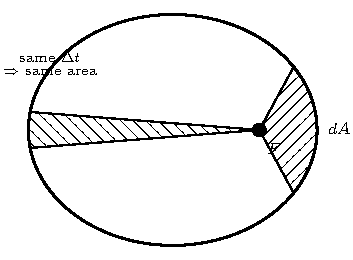
\includegraphics[width=0.42\linewidth]{kepler2}\\
{\footnotesize Equal times $\Rightarrow$ equal areas: the spacecraft is fastest near periapsis.}
\end{center}

\paragraph{Application examples.}
\begin{enumerate}[label=(\arabic*)]
\item \textbf{Angular rate along the orbit.} Writing $\underline v=\dot r\,\hat r+\underline\omega\times\underline r$ with
$\underline\omega=\dot\theta_*\hat h$: $\underline h=\underline r\times(\underline\omega\times\underline r)=\underline\omega r^2$, so
\begin{equation}
\dot\theta_*=\frac{h}{r^2}=\sqrt{\frac{\mu}{p^3}}\left(1+e\,c_{\theta_*}\right)^2 ,
\end{equation}
the differential equation that relates true anomaly and time (basis of Kepler's equation): the motion is fastest at periapsis.
\item \textbf{Horizontal velocity.} $h=r\,v_\theta$ $\Rightarrow$ $v_\theta=h/r$. At the apses ($v_r=0$):
$r_p v_p=r_A v_A=h$, hence $v_p>v_A$ (consistent with the 2nd law).
\item \textbf{Shape of the orbit.} Combined with the eccentricity vector $\underline e=-\hat r+\underline v\times\underline h/\mu$
it gives the polar equation $r=\dfrac{h^2/\mu}{1+e\,c_{\theta_*}}$: the semilatus rectum is $p=h^2/\mu$.
\item \textbf{Orientation of the orbit plane.} $\hat h$ gives the inclination $c_i=\hat h\cdot\hat c_3$ and, with the node
line $\hat c_3\times\underline h$, the RAAN $\Omega$.
\item \textbf{Circular orbits.} $r=R$ and $h=$ const $\Rightarrow$ $\underline\omega=\underline h/R^2$ constant: uniform motion.
\item \textbf{Rectilinear trajectories.} $h=0$ iff $\underline v\parallel\underline r$: $p=0$, $e=1$, the motion is along a line
through the attracting body.
\item \textbf{Impulsive manoeuvres (Ch.\,3).} After an impulse at radius $r$: $h^+=r\,v_\theta^+$, then
$e^+=\sqrt{1-h^{+2}/(\mu a^+)}$; in the Hohmann proof $v_+c_\phi=h^+/R_k=\sqrt{\mu p^+}/R_k$.
\item \textbf{Perturbed motion (Ch.\,8).} With a perturbing acceleration $\underline f$ the integral is lost:
$\dot{\underline h}=\underline r\times\underline f$. Only the out-of-plane component $f_h$ rotates the plane (changes $i$,
$\Omega$); e.g.\ third-body perturbations make $\underline h$ precess.
\end{enumerate}

\begin{keyf}
$\underline h=\underline r\times\underline v$, \quad $\dfrac{d\underline h}{dt}=\underline v\times\underline v+\underline r\times\left(-\dfrac{\mu}{r^2}\hat r\right)=\underline 0$,
\quad $h=2\,\dfrac{dA}{dt}$, \quad $\dot\theta_*=\dfrac{h}{r^2}$, \quad $p=\dfrac{h^2}{\mu}$, \quad $h=r\,v_\theta=r_pv_p=r_Av_A$.
\end{keyf}

\pitfalls
\begin{itemize}
\item State the hypothesis explicitly: \emph{central} force (restricted two-body problem, spherical attracting body).
The proof fails for any non-central perturbation.
\item Say \emph{why} each term vanishes ($\underline v\times\underline v=\underline 0$; $\underline r\parallel\ddot{\underline r}$).
\item $h$ is constant as a \emph{vector}: magnitude (2nd law) and direction (planar motion). Mention both consequences.
\item $\underline h$ and $\underline e$ give 5 independent scalar integrals, not 6, because $\underline h\cdot\underline e=0$.
\end{itemize}

\further
The angular momentum integral is the orbital analogue of the conservation of angular momentum of a system subject to
central (internal) forces: in the $N$-body problem the total $\underline H_c$ about the centre of mass is conserved and
defines the invariant Laplace plane (\qref{B6}).

\source{cap02.tex, \S First Integrals (l.168--201), \S Position in time (l.589--615), \S Circular orbits (l.797--848);
cap03.tex l.51--75; cap08.tex l.87--116. Formulario: \fml{2-HEV}, \fml{2-TDT}.}

% ---------------------------------------------------------------------
\question{A2}{Classification of Keplerian orbits in terms of $a$ and $e$}
% source: cap02.tex l.253-300 (cartesian eq.), 300-371 (conics), 554-587 (energy), 881-927 (rectilinear, classification)
\begin{qbox}
Describe the general classification of Keplerian orbits in terms of semi-major axis and eccentricity.
\qmeta{list by chapter (Ch.\,2).}
\end{qbox}

\begin{outline}
\begin{enumerate}
\item First integrals $\underline h$, $\underline e$ $\Rightarrow$ polar equation $r=p/(1+e\,c_{\theta_*})$, $p=h^2/\mu$.
\item Cartesian form $x^2(1-e^2)+y^2+2pex=p^2$: conic section, the attracting body is at a focus.
\item Definition of $a=p/(1-e^2)$ for all conics ($a>0$, $a\to\infty$, $a<0$).
\item Energy $\mathcal E=-\mu/(2a)$: sign of $\mathcal E$ $\leftrightarrow$ type of orbit.
\item Degenerate case $h=0$: rectilinear trajectories ($e=1$), three types.
\item Summary table $\mathcal E$ (or $a$) vs $e$; sketch of the conics.
\end{enumerate}
\end{outline}

\answer
\paragraph{From the first integrals to the conics.} In the restricted two-body problem $\underline h=\underline r\times\underline v$
and $\underline e=-\hat r+\underline v\times\underline h/\mu$ are constant. Projecting $\underline e$ on $\underline r$
($\theta_*$ = true anomaly, angle from $\underline e$ to $\underline r$):
\begin{equation}
r\,e\cos\theta_*=-r+\frac{h^2}{\mu}\;\Longrightarrow\; r=\frac{p}{1+e\cos\theta_*},\qquad p:=\frac{h^2}{\mu}\ \text{(semilatus rectum)}.
\end{equation}
In a frame centred in the attracting body with $x\parallel\hat e$, using $x=r\,c_{\theta_*}$, $y=r\,s_{\theta_*}$:
\begin{equation}
x^{2}\left(1-e^{2}\right)+y^{2}+2p\,e\,x=p^{2}
\end{equation}
which is a conic section with the attracting body at one focus (Kepler's 1st law):
\begin{itemize}
\item $0\le e<1$: \textbf{ellipse} (circle with the body at the centre if $e=0$);
\item $e=1$: \textbf{parabola} ($y^2+2px=p^2$, $r_p=p/2$);
\item $e>1$: \textbf{hyperbola} (one branch, the one around the focus).
\end{itemize}

\paragraph{Semi-major axis.} Completing the square gives, for the ellipse, semi-axes $a=\dfrac{p}{1-e^2}$,
$b=\dfrac{p}{\sqrt{1-e^2}}$, focal distance $c=ae$. By \emph{convention} the same definition is kept for hyperbolas,
\begin{equation}
a=\frac{p}{1-e^{2}}\quad\Rightarrow\quad a>0\ (e<1),\qquad a\to\infty\ (e=1),\qquad a<0\ (e>1),
\end{equation}
so that $r_p=a(1-e)$ holds for every conic and $r_A=a(1+e)$ for the ellipse.

\paragraph{Energy.} The specific energy $\mathcal E=\frac{v^2}{2}-\frac{\mu}{r}$ is a further integral. Inserting $r(\theta_*)$ and
the speed $v=\sqrt{\mu/p}\,\sqrt{1+e^2+2e\,c_{\theta_*}}$, the dependence on $\theta_*$ cancels:
\begin{equation}
\mathcal E=-\frac{\mu}{2p}\left(1-e^{2}\right)=-\frac{\mu}{2a}.
\end{equation}
Hence the sign of $\mathcal E$ (equivalently of $a$) classifies the orbit:
\begin{center}
\small
\begin{tabular}{@{}lllll@{}}
\toprule
orbit & $e$ & $a$ & $\mathcal E$ & potential vs kinetic energy\\
\midrule
circle & $0$ & $=r$ & $<0$ & $|\mathrm{PE}|=2\,\mathrm{KE}$\\
ellipse (closed, periodic) & $0<e<1$ & $>0$ & $<0$ & $|\mathrm{PE}|>\mathrm{KE}$\\
parabola (escape, $v_\infty=0$) & $1$ & $\infty$ & $=0$ & $|\mathrm{PE}|=\mathrm{KE}$\\
hyperbola (escape, $v_\infty>0$) & $>1$ & $<0$ & $>0$ & $|\mathrm{PE}|<\mathrm{KE}$\\
\bottomrule
\end{tabular}
\end{center}
Characteristic quantities: ellipse $r_{p,A}=a(1\mp e)$, $T=2\pi\sqrt{a^3/\mu}$; parabola $v=\sqrt{2\mu/r}\to0$ at infinity;
hyperbola $v_\infty=\sqrt{-\mu/a}$, true anomaly limited to $|\theta_*|<\theta_*^M=\arccos(-1/e)$, deflection
$\xi=2\theta_*^M-\pi$.

\paragraph{Degenerate case: rectilinear trajectories ($h=0$).} If $\underline v\parallel\underline r$ then $\underline h=\underline 0$,
$e=|-\hat r|=1$, $p=0$, $r_p=0$: the motion is along a straight line through the attracting body ($\theta_*=\pm\pi$). Three
types, classified again by $a$ (or $\mathcal E$):
$a>0,\ \mathcal E<0$ \emph{rectilinear ellipse} (segment: the body falls back);
$a\to\infty,\ \mathcal E=0$ \emph{rectilinear parabola} ($v\to0$ as $r\to\infty$);
$a<0,\ \mathcal E>0$ \emph{rectilinear hyperbola} ($v\not\to0$).

\paragraph{Summary.} A Keplerian path is identified by \textbf{$a$ (or $\mathcal E$) and $e$}:
\begin{center}
\small
\begin{tabular}{@{}c|c|c|c@{}}
\toprule
$\mathcal E$ & $0\le e<1$ & $e=1$ & $e>1$\\
\midrule
$>0$ ($a<0$) & -- & rectilinear hyperbola & hyperbola\\
$=0$ ($a\to\infty$) & -- & parabola, rectilinear parabola & --\\
$<0$ ($a>0$) & ellipse & rectilinear ellipse & --\\
\bottomrule
\end{tabular}
\end{center}
Conic sections have $h\neq0$, $e\ge0$; rectilinear trajectories have $h=0$, $e=1$. Given $r$ and $v$ at any point:
$a=\left(\frac{2}{r}-\frac{v^2}{\mu}\right)^{-1}$ (vis-viva) and $e=\sqrt{1-\frac{h^2}{\mu a}}$.

\begin{center}
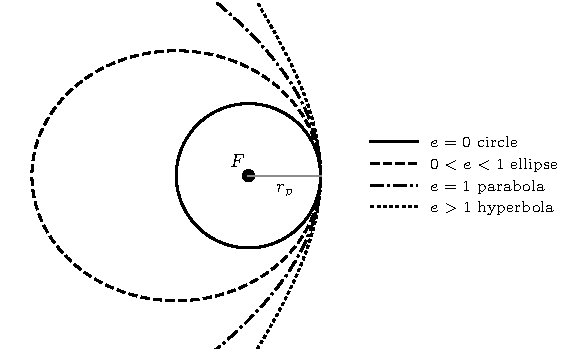
\includegraphics[width=0.62\linewidth]{conics}\\
{\footnotesize Conics with the same periapsis radius $r_p$: $e$ increases from the circle to the hyperbola.}
\end{center}

\begin{fig2draw}
Focus $F$ and a common periapsis; circle, an ellipse closing behind, the parabola (arms becoming parallel) and the
hyperbola (arms approaching the asymptotes, more open than the parabola). Write $e$ and the sign of $a$, $\mathcal E$ on each.
\end{fig2draw}

\begin{keyf}
$r=\dfrac{p}{1+e\,c_{\theta_*}}$, \quad $p=\dfrac{h^2}{\mu}=a(1-e^2)$, \quad $\mathcal E=\dfrac{v^2}{2}-\dfrac{\mu}{r}=-\dfrac{\mu}{2a}$,
\quad $e=\sqrt{1-\dfrac{h^2}{\mu a}}$, \quad $v_\infty=\sqrt{-\mu/a}$.
\end{keyf}

\pitfalls
\begin{itemize}
\item The convention $a<0$ for hyperbolas: forgetting it gives $r_p<0$ or imaginary $v_\infty$.
\item Do not forget the \emph{rectilinear} (degenerate) trajectories: they share $e=1$ with the parabola but have any $\mathcal E$.
\item The circle is the special ellipse $e=0$ (attracting body at the centre), not a separate class.
\item $e$ alone does not identify the orbit size; $a$ alone does not identify the shape: both are needed.
\end{itemize}

\source{cap02.tex l.230--300 (polar and Cartesian equations), l.300--371 (ellipse, parabola, hyperbola), l.554--587 (energy),
l.881--927 (rectilinear trajectories, classification table), l.929--945 (vis-viva). Formulario: \fml{2-POL}, \fml{2-ENE}, \fml{2-VIS}.}

% ---------------------------------------------------------------------
\question{A3}{Trajectories from a horizontal velocity at a given altitude}
% source: cap02.tex l.532-552 (cosmic velocities), l.929-1005 (cases a-g), l.870-879 (ballistic)
\begin{qbox}
A spacecraft is at a specified altitude above Earth and has horizontal velocity. Describe the different Keplerian
trajectories it can follow for various velocity magnitudes.
\qmeta{list by chapter (Ch.\,2).}
\end{qbox}

\begin{outline}
\begin{enumerate}
\item Data: $r=R_E+$altitude, $\underline v_0\perp\underline r$ $\Rightarrow$ $P_0$ is an apse ($v_r=0$).
\item Cosmic velocities $v_I=\sqrt{\mu/r}$ (circular), $v_{II}=\sqrt{2\mu/r}$ (escape).
\item $a$ from vis-viva, $e$ from $h=rv_0$: $e=|v_0^2/v_I^2-1|$.
\item Seven cases (a)--(g) with sketch; $P_0$ apoapsis below $v_I$, periapsis above.
\item Remark: low $v_0$ $\Rightarrow$ periapsis inside the Earth: ballistic arc (impact).
\end{enumerate}
\end{outline}

\answer
\paragraph{Data and cosmic velocities.} Let $P_0$ be at distance $r$ from the Earth's centre ($r=R_E+\text{altitude}$) and let
the velocity $\underline v_0$ be horizontal, i.e.\ orthogonal to $\underline r$. Two \emph{cosmic velocities} are defined at $P_0$:
\begin{equation}
v_I=\sqrt{\frac{\mu}{r}}\ \ \text{(1st: circular orbit of radius $r$)},\qquad
v_{II}=\sqrt{\frac{2\mu}{r}}=\sqrt2\,v_I\ \ \text{(2nd: escape, parabola)}.
\end{equation}

\paragraph{Orbit elements as functions of $v_0$.} With $\underline v_0\perp\underline r$: $v_r=0$, so $P_0$ is an apse (periapsis or
apoapsis), and $h=r\,v_0$. Vis-viva and angular momentum give
\begin{equation}
a=\frac{1}{\dfrac{2}{r}-\dfrac{v_0^{2}}{\mu}},\qquad p=\frac{h^2}{\mu}=r\,\frac{v_0^2}{v_I^2},\qquad
e=\left|\frac{p}{r}-1\right|=\left|\frac{v_0^{2}}{v_I^{2}}-1\right|,
\end{equation}
the last one because at an apse $r=p/(1\pm e)$. With $k=v_0^2/v_I^2$ the \emph{other} apse is at $r'=r\,k/(2-k)$.
As $v_0$ grows, $\mathcal E=\frac{v_0^2}{2}-\frac{\mu}{r}$ grows monotonically.

\paragraph{The cases.}
\begin{enumerate}[label=(\alph*)]
\item $v_0=0$: \textbf{rectilinear ellipse}, straight fall towards the centre ($h=0$, $e=1$, $a=r/2$).
\item $0<v_0<v_I$: \textbf{ellipse with $P_0$ as apoapsis} ($e=1-k$); the periapsis radius $r_p=r\,k/(2-k)$ increases with $v_0$.
If $r_p<R_E$ the ellipse intersects the Earth's surface: the path is a \emph{ballistic trajectory} (arc of ellipse with
periapsis inside the Earth, as for ICBMs) and the spacecraft re-enters/impacts.
\item $v_0=v_I$: \textbf{circular orbit} of radius $r$ ($e=0$, $a=r$).
\item $v_I<v_0<v_{II}$: \textbf{ellipse with $P_0$ as periapsis} ($e=k-1$); the apoapsis radius $r_A=r\,k/(2-k)$ increases
with $v_0$ and tends to infinity as $v_0\to v_{II}$.
\item $v_0=v_{II}$: \textbf{parabola} with periapsis $r_p=r$ ($e=1$, $\mathcal E=0$): escape with zero velocity at infinity.
\item $v_0>v_{II}$: \textbf{hyperbola} with periapsis at $P_0$; $e$ increases with $v_0$, $v_\infty=\sqrt{v_0^2-v_{II}^2}$.
\item $v_0\to\infty$: $e\to\infty$, the path tends to the \textbf{straight line} orthogonal to $\underline r$ (gravity has no time to bend it).
\end{enumerate}

\begin{center}
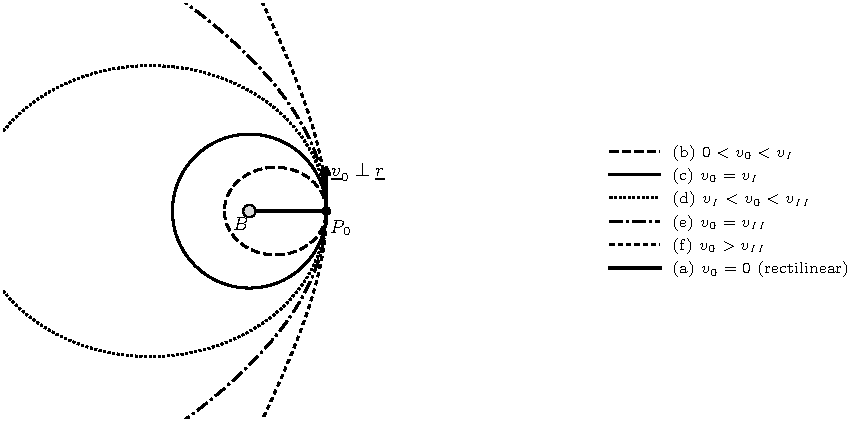
\includegraphics[width=0.86\linewidth]{vhoriz}\\
{\footnotesize Paths computed with $r=p/(1+e\cos\theta_*)$ for $v_0/v_I=0.7,\ 1,\ 1.25,\ \sqrt2,\ 1.75$.}
\end{center}

\begin{fig2draw}
Earth centre $B$, point $P_0$ to its right, short arrow $\underline v_0$ upwards. Draw: small ellipse inside (apoapsis at $P_0$),
circle through $P_0$, larger ellipse outside (periapsis at $P_0$), parabola and hyperbola opening to the left, and
the radial segment $BP_0$ for $v_0=0$. Label each with the velocity interval.
\end{fig2draw}

\begin{keyf}
$v_I=\sqrt{\mu/r}$, \ $v_{II}=\sqrt{2\mu/r}$, \ $a=\left(\dfrac2r-\dfrac{v_0^2}{\mu}\right)^{-1}$, \ $e=\left|\dfrac{v_0^2}{v_I^2}-1\right|$,
\ $h=rv_0$, \ other apse $r'=r\dfrac{k}{2-k}$, $k=\dfrac{v_0^2}{v_I^2}$.
\end{keyf}

\pitfalls
\begin{itemize}
\item Below $v_I$ the starting point is the \emph{apoapsis}, above $v_I$ it is the \emph{periapsis}.
\item $v_{II}=\sqrt2\,v_I$ holds at the same $r$; the escape speed is not "infinite energy".
\item Mention the physical limit: for small $v_0$ the periapsis falls inside the Earth (ballistic arc).
\end{itemize}

\source{cap02.tex l.532--552 (cosmic velocities), l.870--879 (ballistic trajectories), l.929--1005 (cases (a)--(g)).
The closed-form $e=|v_0^2/v_I^2-1|$ and $r'$ follow from the notes' formulas. Formulario: \fml{2-COS}, \fml{2-V0C}.}

% ---------------------------------------------------------------------
\question{A4}{Geosynchronous and geostationary orbits; ground tracks}
% source: cap02.tex l.850-868 (geosynchronous), l.1657-1843 (ground track), cap08 l.80-85 (J22 resonance)
\begin{qbox}
Define geosynchronous and geostationary orbits, commenting on their properties. Provide a graphical representation of the
ground track for zero/non-zero inclination and zero/non-zero eccentricity.
\qmeta{Jan 2023.}
\end{qbox}

\begin{outline}
\begin{enumerate}
\item Sidereal day $T_{sid}=2\pi/\omega_E=86164$\,s; geosynchronous: $T=T_{sid}$ $\Rightarrow$ $a=42164$\,km, any $e$, $i$.
\item Geostationary = geosynchronous + $e=0$ + $i=0$: fixed sub-satellite point on the equator.
\item Ground track definition: $\phi(t)$, $\lambda_g(t)=\xi-\theta_g$; $\phi=\arcsin(s_{\theta_t}s_i)$, latitude band $\pm i$.
\item Four sketches: ($i=0,e=0$) point; ($i\neq0,e=0$) figure eight; ($i=0,e\neq0$) segment on the equator;
($i\neq0,e\neq0$) distorted eight/drop, depending on $\omega$.
\item Properties: closed track for direct orbits (repeats every day); symmetries; motion E/W; uses and perturbations.
\end{enumerate}
\end{outline}

\answer
\paragraph{Definitions.} The \emph{sidereal day} is the time the Earth takes for one rotation with respect to an inertial frame:
$T_{sid}=2\pi/\omega_E=86164$\,s ($\omega_E=7.292115\cdot10^{-5}$\,rad/s), shorter than the solar day (86400\,s).
An orbit is \textbf{geosynchronous} if its period equals one sidereal day:
\begin{equation}
2\pi\sqrt{\frac{a^{3}}{\mu_{E}}}=T_{\text{sid}}\;\Longrightarrow\;
a_{gs}=\left[\mu_{E}\left(\frac{T_{\text{sid}}}{2\pi}\right)^{2}\right]^{1/3}=42164\ \text{km}
\end{equation}
(altitude $\approx35786$\,km for a circular orbit). \emph{No assumption is made on $i$ and $e$}, apart from a periapsis high
enough to avoid the atmosphere.

An orbit is \textbf{geostationary} if it is at the same time (1) geosynchronous ($a=42164$\,km), (2) circular ($e=0$),
(3) equatorial ($i=0$). The satellite then moves with the same angular velocity as the Earth, in the same plane and
direction: the sub-satellite point is a \textbf{fixed point on the equator} and the satellite appears motionless to a
ground observer. Geostationary orbits are a subset of geosynchronous orbits.

\paragraph{Ground track.} It is the locus of the sub-satellite points (projection of the satellite on the rotating Earth),
plotted on a Mercator map as latitude $\phi(t)$ vs geographical longitude $\lambda_g(t)$:
\begin{equation}
s_\phi=s_{\theta_t}s_i,\qquad \lambda_g=\xi-\theta_g,\qquad \theta_g=\theta_{g0}+\omega_E(t-t_0),
\end{equation}
with $\theta_t=\omega+\theta_*$ (argument of latitude), $\xi$ the absolute (inertial) longitude and $\theta_g$ the
longitude of Greenwich. For direct orbits $-i\le\phi\le i$.

\paragraph{The four cases} (tracks computed with Kepler's equation, $a=42164$\,km):
\begin{itemize}
\item \textbf{$i=0$, $e=0$} (geostationary): a single \textbf{point} on the equator.
\item \textbf{$i\neq0$, $e=0$}: a symmetric \textbf{figure eight} between latitudes $\pm i$, centred on the equator, with the
crossing point at the equator. The satellite moves at constant inertial speed, but its eastward component varies with
latitude, so it alternately leads and lags the Earth (small longitude excursion, $\propto i^2$). Symmetric w.r.t.\ the
meridian through $\phi_{\max}$ and w.r.t.\ the equator crossing (both symmetries, $e=0$).
\item \textbf{$i=0$, $e\neq0$}: a \textbf{segment on the equator} travelled back and forth once a day: near perigee the satellite
is faster than the Earth (moves east), near apogee slower (moves west); the amplitude grows with $e$ (about $\pm2e$\,rad
for small $e$ \notinnotes).
\item \textbf{$i\neq0$, $e\neq0$}: a \textbf{distorted (asymmetric) eight} or a \textbf{drop/loop} shape, still closed. The shape depends on
$\omega$: with $\omega=0,\pi$ the track is symmetric w.r.t.\ the points where it crosses the equator; with $\omega=\pm\pi/2$
it is symmetric w.r.t.\ the meridian through the maximum and minimum latitudes (apocentre/pericentre).
\end{itemize}
\begin{center}
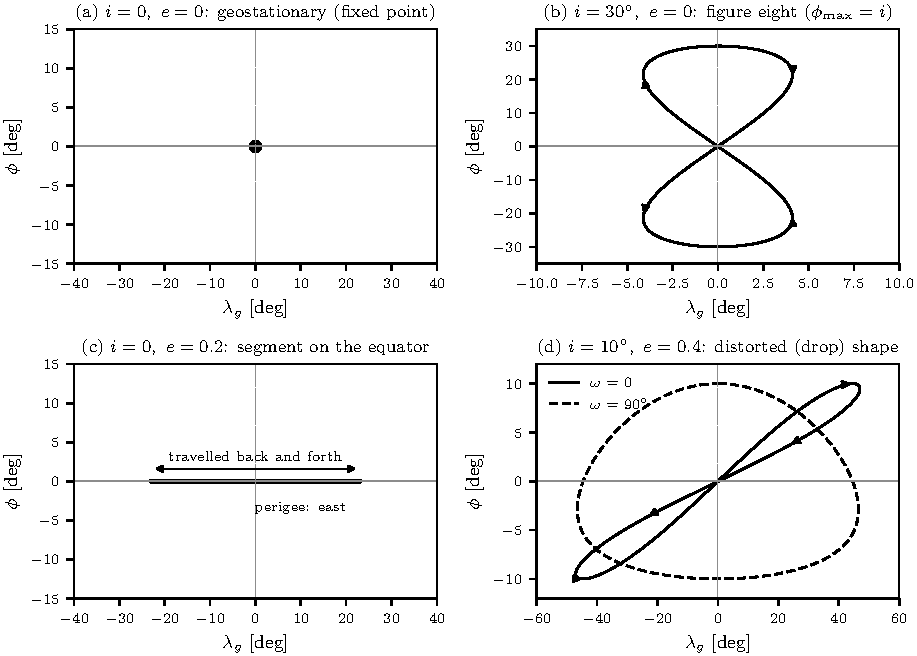
\includegraphics[width=0.95\linewidth]{geosync}
\end{center}

\paragraph{Properties.}
\begin{itemize}
\item Since the period is one sidereal day, the motion is synchronous with the Earth's rotation and the \textbf{track repeats
every day}. For direct orbits ($0<i<\pi/2$) the track is \textbf{closed} and spans a limited range of longitudes; it is travelled
partly towards East and partly towards West. For retrograde geosynchronous orbits ($\pi/2<i<\pi$) the track is repeating
but covers all longitudes (always travelled westward).
\item General rule: after one period a direct track drifts east if $T<T_{sid}$, west if $T>T_{sid}$; geosynchronous is the
boundary case with zero drift.
\item Geostationary orbits give continuous coverage of about one third of the Earth with fixed antennas
(telecommunications, meteorology); they cannot see the polar regions.
\item Perturbations: at GEO the dominant one is the sectoral harmonic $J_{22}$ (ellipticity of the equator), amplified by
resonance because the satellite is fixed with respect to the Earth; Sun and Moon make $i$ grow, SRP changes $e$
$\Rightarrow$ station keeping is needed.
\end{itemize}

\begin{fig2draw}
Four small $\lambda_g$--$\phi$ frames: a dot at the origin; an "8" between $\pm i$; a horizontal segment on the equator with a
double arrow; a lopsided "8" (or a drop) for $e\neq0$, with a note on the symmetry given by $\omega$.
\end{fig2draw}

\begin{keyf}
$T_{sid}=\dfrac{2\pi}{\omega_E}=86164$\,s, \quad $a_{gs}=\left[\mu_E\left(\dfrac{T_{sid}}{2\pi}\right)^2\right]^{1/3}=42164$\,km,
\quad $s_\phi=s_{\theta_t}s_i$, \quad $\lambda_g=\xi-\theta_g$.
\end{keyf}

\pitfalls
\begin{itemize}
\item Use the \emph{sidereal} day (86164\,s), not 24\,h.
\item "Geosynchronous" does not imply circular or equatorial; "geostationary" requires all three conditions.
\item The figure eight of the circular inclined case is symmetric and centred on the equator; the eccentric cases are not.
\end{itemize}

\source{cap02.tex l.850--868 (geosynchronous orbits), l.1657--1739 (ground track), l.1741--1796 (latitude limits, symmetry),
l.1798--1855 (geosynchronous and geostationary tracks, motion along the track), l.1857--1960 (examples 1--3);
cap08.tex l.80--85 ($J_{22}$ at GEO). Formulario: \fml{2-GEO}, \fml{2-GTK}, \fml{2-GTD}.}

% ---------------------------------------------------------------------
\question{A5}{Impulsive-thrust approximation}
% source: cap03.tex l.18-113
\begin{qbox}
Describe the impulsive-thrust approximation -- its validity assumptions and the change in position and velocity due to an
impulsive $\Delta V$. Give one mission scenario where the approximation is valid and one where it is not.
\qmeta{list by chapter (Ch.\,3).}
\end{qbox}

\begin{outline}
\begin{enumerate}
\item Idea: high thrust for a short time $\Rightarrow$ instantaneous velocity change; limit $T\to\infty$, $\Delta t\to0$, $T\Delta t=\Delta v$ finite.
\item Effects: $\underline r^+=\underline r^-$, $\underline v^+=\underline v^-+\Delta\underline v$ (magnitude and direction).
\item Validity: burn time $\ll$ orbital period, negligible displacement and gravity/drag effects during the burn; optimistic estimate.
\item New orbit: $a^+$ from energy, $e^+$ from $h$, $\theta_*^+$ from $r$ and $v_r$; apsidal line rotates.
\item Examples: valid (chemical orbit transfers, Hohmann, injection); not valid (launcher ascent, low-thrust).
\end{enumerate}
\end{outline}

\answer
\paragraph{The approximation.} If a \textbf{high thrust} acts for a \textbf{short time} $\Delta t$, its effect can be approximated as an
\emph{instantaneous} change of velocity, while the position does not change. Mathematically (thrust per unit mass $T$)
\begin{equation}
T\,\Delta t=\Delta v,
\end{equation}
and the impulsive approximation is the limit $T\to\infty$, $\Delta t\to0$ with the product $T\Delta t=\Delta v$ finite. Through a
\textbf{velocity impulse}: (a) the velocity changes in direction and magnitude; (b) the position does not change.

\paragraph{Validity assumptions.}
\begin{itemize}
\item High-thrust propulsion (chemical engines): the burn duration is very short compared with the orbital period, so the
spacecraft moves negligibly during the burn and the change of $\underline r$ is negligible.
\item During the burn gravity (and drag) do not change the velocity appreciably: no gravity/drag losses; Tsiolkovsky's law
can be used to compute the propellant.
\item The result is an \emph{optimistic} guess for real scenarios (finite burns always cost a little more).
\end{itemize}

\paragraph{Effect of an impulse.} At $P$ (true anomaly $\theta_*^-$ on the old orbit):
\begin{equation}
\underline r^+=\underline r^-,\qquad \underline v^+=\underline v^-+\Delta\underline v,\qquad
\Delta\underline v=\Delta v_\theta\,\hat\theta+\Delta v_r\,\hat r .
\end{equation}
With $v_r^-=\sqrt{\mu/p^-}\,e^-s_{\theta_*^-}$ and $v_\theta^-=\sqrt{\mu/p^-}\,(1+e^-c_{\theta_*^-})$:
\begin{equation}
v_r^+=v_r^-+\Delta v_r,\qquad v_\theta^+=v_\theta^-+\Delta v_\theta .
\end{equation}
The new orbit follows in three steps:
\begin{enumerate}
\item $a^+$ from the \textbf{energy}: $\dfrac{(v^+)^2}{2}-\dfrac{\mu}{r}=-\dfrac{\mu}{2a^+}\Rightarrow a^+=\dfrac{\mu}{2\mu/r-(v^+)^2}$;
\item $e^+$ from the \textbf{angular momentum}: $h^+=r\,v_\theta^+=\sqrt{\mu a^+[1-(e^+)^2]}\Rightarrow e^+=\sqrt{1-\dfrac{h^{+2}}{\mu a^+}}$;
\item $\theta_*^+$ from \textbf{radius and radial velocity}: $c_{\theta_*^+}=\dfrac{p^+-r}{r\,e^+}$, $s_{\theta_*^+}=\dfrac{v_r^+}{e^+}\sqrt{\dfrac{p^+}{\mu}}$
$\Rightarrow\theta_*^+=2\operatorname{atan}\dfrac{s_{\theta_*^+}}{1+c_{\theta_*^+}}$ (correct quadrant).
\end{enumerate}
The apsidal line rotates by $\theta_*^--\theta_*^+$; the vacant focus moves so that the new velocity satisfies the reflection
property of the new ellipse. A tangential impulse ($\Delta v_r=0$ at an apse) does not rotate the apsidal line.

\begin{center}
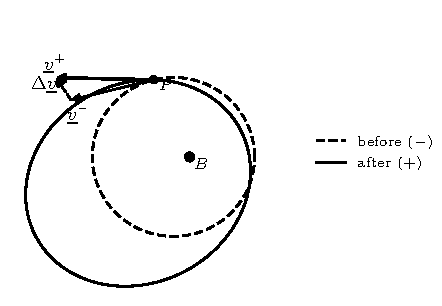
\includegraphics[width=0.55\linewidth]{impulse}\\
{\footnotesize Same position, new velocity: the orbit through $P$ changes shape and orientation.}
\end{center}

\paragraph{Examples.}
\begin{itemize}
\item \textbf{Valid}: orbit transfers with chemical engines (e.g.\ LEO$\to$GEO Hohmann transfer: burns of a few minutes vs
orbital periods of hours; plane changes at the nodes; injection into an escape hyperbola; rendezvous burns). The
Bounded Multi Impulse model, used to approximate finite burns, is itself based on impulsive $\Delta v$'s.
\item \textbf{Not valid}: (a) the ascent trajectory of a launch vehicle (thrust acts for minutes while gravity and drag
cause large losses and the position changes by hundreds of km); (b) low-thrust trajectories (electric propulsion), where
continuous thrust is applied for long time intervals (weeks or months) and the orbit spirals.
\end{itemize}

\begin{keyf}
$T\Delta t=\Delta v$ ($T\to\infty$, $\Delta t\to0$), \quad $\underline r^+=\underline r^-$, \quad $\underline v^+=\underline v^-+\Delta\underline v$,
\quad $a^+=\dfrac{\mu}{2\mu/r-(v^+)^2}$, \quad $e^+=\sqrt{1-\dfrac{(r\,v_\theta^+)^2}{\mu a^+}}$.
\end{keyf}

\pitfalls
\begin{itemize}
\item The position does \emph{not} change: the old and new orbits intersect at $P$.
\item Say that the approximation is optimistic and requires a burn time much shorter than the orbital period.
\item Use the radial \emph{and} horizontal components; $\theta_*^+$ needs both $\sin$ and $\cos$ for the quadrant.
\end{itemize}

\source{cap03.tex l.18--43 (approximation, validity), l.45--113 (effect of velocity impulses). Formulario: \fml{3-IMP}, \fml{3-NEW}.}

% ---------------------------------------------------------------------
\question{A6}{Hohmann transfer vs bielliptic transfer}
% source: cap03.tex l.115-377
\begin{qbox}
Compare a Hohmann transfer with a bielliptic transfer (between circular coplanar orbits), discussing the conditions under
which each option is optimal.
\qmeta{$\times$2 in the list (2025); Jan 2025; Jun 2025 ("discussing the conditions under which each option is optimal").}
\end{qbox}

\begin{outline}
\begin{enumerate}
\item Problem: coplanar circular orbits $R_i\to R_f$, minimise $\Delta v_{tot}$ (= propellant).
\item Hohmann: bitangent ellipse, $a_T$, $e_T$, $\Delta v_1$, $\Delta v_2$, $\Delta t=\pi\sqrt{a_T^3/\mu}$; globally optimal among 2-impulse transfers (sketch of proof).
\item Bielliptic: 3 impulses, intermediate apoapsis $r_A^{\max}$, $\Delta v_{1,2,3}$, $\Delta t$; biparabolic limit.
\item Non-dimensional comparison $\sigma=R_f/R_i$, $\rho=r_A^{\max}/R_i\ge\sigma$; plot.
\item Result: $\sigma<11.94$ Hohmann; $11.94<\sigma<15.58$ depends on $\rho$; $\sigma>15.58$ bielliptic. Trade-off with time of flight.
\end{enumerate}
\end{outline}

\answer
\paragraph{Problem.} Given two coplanar circular orbits of radii $R_i$ and $R_f$ ($R_f>R_i$), find the impulsive transfer that
minimises $\Delta v_{tot}$, i.e.\ the propellant consumption (Tsiolkovsky).

\paragraph{Hohmann transfer.} The transfer arc is an ellipse tangent to both circles (bitangent), with periapsis on the
initial orbit and apoapsis on the final one:
\begin{equation}
a_{T}=\frac{R_{i}+R_{f}}{2},\qquad e_{T}=\frac{R_{f}-R_{i}}{R_{f}+R_{i}} .
\end{equation}
Two impulses, both \emph{tangent and in the direction of motion} (both increase $a$):
\begin{equation}
\Delta v_{1}=\sqrt{\frac{2\mu}{R_{i}+R_{f}}\frac{R_{f}}{R_{i}}}-\sqrt{\frac{\mu}{R_{i}}},\qquad
\Delta v_{2}=\sqrt{\frac{\mu}{R_{f}}}-\sqrt{\frac{2\mu}{R_{i}+R_{f}}\frac{R_{i}}{R_{f}}},\qquad
\Delta t=\pi\sqrt{\frac{a_{T}^{3}}{\mu}} .
\end{equation}
\emph{Optimality.} Among all two-impulse transfers with an elliptic arc, the feasible ones satisfy $r_{P_T}\le R_i$ and
$r_{A_T}\ge R_f$. For each impulse
$(\Delta v_k)^2=\frac{3\mu}{R_k}-2\frac{\mu}{R_k}\sqrt{\frac{p_T}{R_k}}-\frac{\mu}{p_T}(1-e_T^2)$, and
$\partial(\Delta v_k)^2/\partial e_T=2e_T\mu/p_T>0$: at fixed $p_T$ the cost grows with $e_T$; along both boundaries of the
feasible region $d(\Delta v_1+\Delta v_2)/de_T>0$ too. Hence the minimum is at the corner point $H$ where both constraints
are active, the bitangent ellipse: the Hohmann transfer is the \textbf{globally optimal two-impulse} transfer.

With $\sigma=R_f/R_i$:
$\dfrac{\Delta v^{(H)}_{tot}}{\sqrt{\mu/R_i}}=\sqrt{\dfrac{2\sigma}{1+\sigma}}-1+\dfrac{1}{\sqrt\sigma}-\sqrt{\dfrac{2}{\sigma(1+\sigma)}}$;
it has a \textbf{maximum at $\sigma\simeq15.58$} and the asymptote $\sqrt2-1$ (transfer to a parabola) as $\sigma\to\infty$.

\paragraph{Bielliptic transfer.} Three impulses and two half-ellipses with a common apoapsis $r_A^{\max}\ge R_f$:
\begin{equation}
\sys{\Delta v_{1}^{(BE)}&=\sqrt{\tfrac{2\mu}{R_{i}+r_{A}^{\max}}\tfrac{r_{A}^{\max}}{R_{i}}}-\sqrt{\tfrac{\mu}{R_{i}}}
&&\text{(at $R_i$, along the motion)}\\
\Delta v_{2}^{(BE)}&=\sqrt{\tfrac{2\mu}{R_{f}+r_{A}^{\max}}\tfrac{R_{f}}{r_{A}^{\max}}}-\sqrt{\tfrac{2\mu}{R_{i}+r_{A}^{\max}}\tfrac{R_{i}}{r_{A}^{\max}}}
&&\text{(at $r_A^{\max}$: raises the periapsis to $R_f$)}\\
\Delta v_{3}^{(BE)}&=\sqrt{\tfrac{2\mu}{R_{f}+r_{A}^{\max}}\tfrac{r_{A}^{\max}}{R_{f}}}-\sqrt{\tfrac{\mu}{R_{f}}}
&&\text{(at $R_f$, \emph{opposite} to the motion: circularises)}}
\end{equation}
\begin{equation}
\Delta t=\pi\sqrt{\frac{a_{T1}^{3}}{\mu}}+\pi\sqrt{\frac{a_{T2}^{3}}{\mu}},\qquad a_{T1}=\frac{R_i+r_A^{\max}}{2},\ a_{T2}=\frac{R_f+r_A^{\max}}{2}.
\end{equation}
As $r_A^{\max}$ increases $\Delta v_{tot}$ decreases but $\Delta t$ increases. The limit $r_A^{\max}\to\infty$ is the
\textbf{biparabolic transfer}: $\Delta v_1=(\sqrt2-1)\sqrt{\mu/R_i}$, $\Delta v_2=0$, $\Delta v_3=(\sqrt2-1)\sqrt{\mu/R_f}$,
$\Delta t=\infty$ (best of all bielliptic transfers, but infeasible). The idea: the expensive part of the plane-raising is done
far away, where the velocity is small and a small $\Delta v_2$ raises the periapsis a lot.

\begin{center}
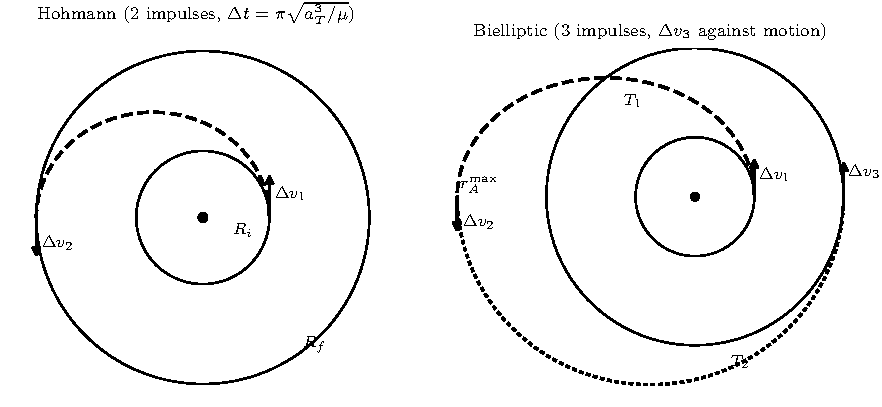
\includegraphics[width=0.9\linewidth]{hoh_be_geom}
\end{center}

\paragraph{Comparison.} With $\sigma=R_f/R_i$ and $\rho=r_A^{\max}/R_i\ge\sigma$ both costs are functions of $(\sigma,\rho)$ only:
\begin{center}
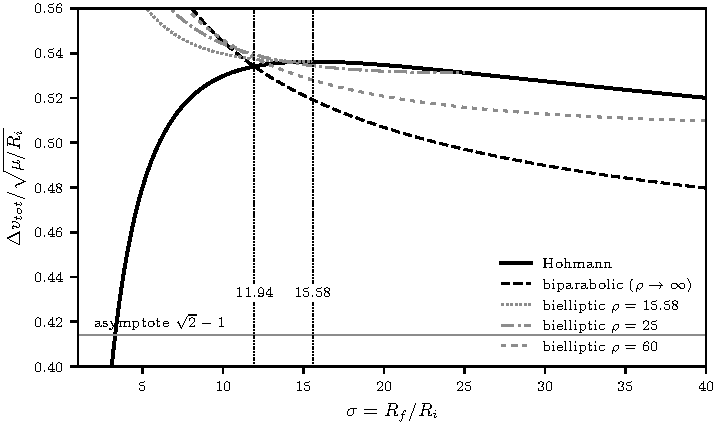
\includegraphics[width=0.72\linewidth]{hoh_be_dv}\\
{\footnotesize $\Delta v_{tot}/\sqrt{\mu/R_i}$ computed from the formulas above; bielliptic curves exist only for $\sigma\le\rho$.}
\end{center}
\begin{itemize}
\item Hohmann and biparabolic curves intersect at $\sigma=11.94$; both tend to $\sqrt2-1$.
\item For finite $\rho$ the intersection with the Hohmann curve moves towards $\sigma=15.58$ as $\rho$ decreases: all
intersections lie in $11.94\le\sigma\le15.58$.
\end{itemize}
\begin{equation}
\begin{cases}
\sigma<11.94: & \text{Hohmann is globally optimal;}\\
11.94<\sigma<15.58: & \text{either may be optimal, depending on }\rho=r_A^{\max}/R_i\ge\sigma;\\
\sigma>15.58: & \text{the bielliptic transfer is optimal (for any }\rho\ge\sigma).
\end{cases}
\end{equation}

\begin{center}
\small
\begin{tabular}{@{}p{3.4cm}p{5.6cm}p{5.6cm}@{}}
\toprule
 & Hohmann & Bielliptic\\
\midrule
impulses & 2, both along the motion & 3 (two along, the last against the motion)\\
free parameter & none & $r_A^{\max}$ (limited by the mission time)\\
$\Delta v_{tot}$ & minimum for $\sigma<11.94$ & lower for $\sigma>15.58$; gain small (few \%)\\
time of flight & half period of one ellipse & two half periods, much longer (grows with $r_A^{\max}$)\\
optimality & globally optimal among 2-impulse transfers & beats Hohmann only for large $\sigma$\\
practical use & almost always (e.g.\ LEO$\to$GEO: $\sigma\approx6.3$) & rare: large $\sigma$ and no time constraint\\
\bottomrule
\end{tabular}
\end{center}

\begin{keyf}
$a_T=\dfrac{R_i+R_f}{2}$, \ $\Delta v_1=\sqrt{\dfrac{2\mu R_f}{R_i(R_i+R_f)}}-\sqrt{\dfrac{\mu}{R_i}}$, \
$\Delta v_2=\sqrt{\dfrac{\mu}{R_f}}-\sqrt{\dfrac{2\mu R_i}{R_f(R_i+R_f)}}$, \ $\Delta t=\pi\sqrt{a_T^3/\mu}$;
thresholds $\sigma=11.94$ and $15.58$; biparabolic $\Delta v=(\sqrt2-1)(\sqrt{\mu/R_i}+\sqrt{\mu/R_f})$.
\end{keyf}

\pitfalls
\begin{itemize}
\item Hohmann is optimal among \emph{two}-impulse transfers only; three-impulse transfers can do better for large $\sigma$.
\item $\Delta v_3$ of the bielliptic transfer is a braking impulse (opposite to the motion).
\item Always mention the time of flight: the gain of the bielliptic transfer is paid with a much longer transfer.
\item The 15.58 value is also the maximum of the Hohmann cost; 11.94 is the Hohmann--biparabolic crossing.
\end{itemize}

\source{cap03.tex l.115--240 (two-impulse optimality), l.242--284 (Hohmann), l.286--344 (bielliptic, biparabolic), l.346--377
(comparison). Thresholds re-checked numerically in \texttt{figures/src/make\_figures.py}. Formulario: \fml{3-HOH}, \fml{3-BEL}, \fml{3-HVB}.}

% ---------------------------------------------------------------------
\question{A7}{Globally optimal transfers from an elliptic orbit to a hyperbolic path}
% source: cap03.tex l.379-449
\begin{qbox}
Describe two optimal ways to transfer a spacecraft from an elliptical orbit to a hyperbolic trajectory and discuss their
global optimality.
\qmeta{list by chapter (Ch.\,3).}
\end{qbox}

\begin{outline}
\begin{enumerate}
\item Problem: planar; initial ellipse ($r_p$, $r_A$); final hyperbola/parabola with given energy $\mathcal E_f\ge0$; no orientation constraint;
bounds $r_A^{\max}$, $r_p^{\min}$ on intermediate orbits.
\item Why periapsis: at fixed $r$, $\Delta\mathcal E=v\,\Delta v+\Delta v^2/2$ $\Rightarrow$ impulses are most effective where $v$ is largest.
\item Case 1, $\mathcal E_f<\mu/r_A^{\max}$: one tangential impulse at periapsis.
\item Case 2, $\mathcal E_f>\mu/r_A^{\max}$: three impulses (raise apoapsis to $r_A^{\max}$, lower periapsis to $r_p^{\min}$, escape at the new periapsis).
\item Global optimality: these are the globally optimal solutions of the problem; analogy with Hohmann/bielliptic; application to interplanetary injection.
\end{enumerate}
\end{outline}

\answer
\paragraph{Problem statement.} Planar transfer, with no constraint on the orientation of the terminal orbits:
\begin{itemize}
\item initial ellipse with specified $r_A$ and $r_p$;
\item final hyperbola ($\mathcal E_f>0$) or parabola ($\mathcal E_f=0$) with specified specific energy $\mathcal E_f$,
coplanar with the ellipse (only the energy, i.e.\ $v_\infty=\sqrt{2\mathcal E_f}$, matters, not the direction);
\item intermediate orbits are bounded: apoapsis radius $\le r_A^{\max}$ (e.g.\ sphere of influence, time) and periapsis radius
$\ge r_p^{\min}$ (e.g.\ planetary radius plus atmosphere).
\end{itemize}

\paragraph{Why impulses at periapsis.} An impulse does not change $r$, so from $\mathcal E=v^2/2-\mu/r$ a tangential impulse gives
\begin{equation}
\Delta\mathcal E=\frac{(v+\Delta v)^2-v^2}{2}=v\,\Delta v+\frac{\Delta v^2}{2}:
\end{equation}
the same $\Delta v$ produces the largest energy increase where the speed is largest, i.e.\ at periapsis; and the lower the
periapsis, the larger the speed there.

\paragraph{The two globally optimal strategies.}
\begin{enumerate}[label=(\arabic*)]
\item $\mathcal E_f<\mu/r_A^{\max}$: the globally optimal transfer is a \textbf{single tangential impulse at periapsis} that raises
the energy to $\mathcal E_f$:
\begin{equation}
\Delta v=\sqrt{2\left(\mathcal E_f+\frac{\mu}{r_p}\right)}-v_p,\qquad v_p=\sqrt{\frac{\mu}{a}\frac{1+e}{1-e}} .
\end{equation}
\item $\mathcal E_f>\mu/r_A^{\max}$: the globally optimal transfer has \textbf{three impulses}:
\begin{enumerate}[label=(\alph*)]
\item impulse at periapsis, to raise the apoapsis radius to $r_A^{\max}$;
\item impulse at apoapsis (where the speed is small, so it is cheap), to lower the periapsis radius to $r_p^{\min}$;
\item impulse at the new periapsis $r_p^{\min}$, where the speed is now much higher, to increase the energy to $\mathcal E_f$.
\end{enumerate}
\end{enumerate}
\begin{center}
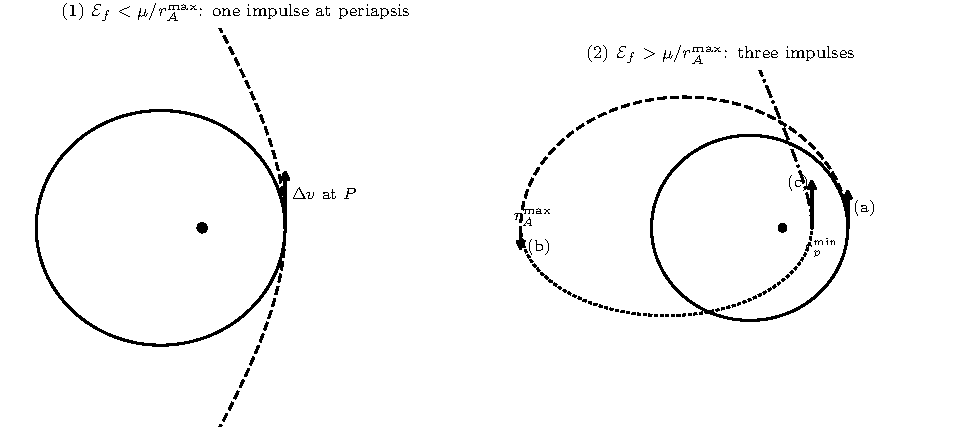
\includegraphics[width=0.92\linewidth]{ell_hyp}
\end{center}

\paragraph{Global optimality (discussion).} The two solutions are the global optima of the problem above, i.e.\ no other
sequence of impulses within the bounds yields a smaller $\Delta v_{tot}$; which one applies depends only on the comparison
between $\mathcal E_f$ and $\mu/r_A^{\max}$. The three-impulse strategy pays two extra impulses to "move" the final burn
to a lower periapsis, which is convenient only when the final energy (the escape burn) is large enough; otherwise the single
periapsis burn is optimal. The logic is the same as for circle-to-circle transfers: the Hohmann transfer is optimal for
moderate changes, the bielliptic one (going far away, where velocity changes are cheap) for large changes. The limiting
values $r_A^{\max}$, $r_p^{\min}$ come from practical constraints (time, sphere of influence, atmosphere, safety).

\paragraph{Application: injection into an interplanetary hyperbola.} From a circular parking orbit of radius $r_p$
the required hyperbolic excess speed $v_\infty$ (from the heliocentric transfer, e.g.\ $v_\infty^{(E)}=\Delta v_1^{(H)}$) fixes
$\mathcal E_f=v_\infty^2/2$, and the single periapsis burn is
$\Delta v=\sqrt{v_\infty^2+2\mu/r_p}-\sqrt{\mu/r_p}$, which is smaller for lower parking orbits.

\begin{keyf}
$\Delta\mathcal E=v\Delta v+\tfrac12\Delta v^2$; \ case 1 ($\mathcal E_f<\mu/r_A^{\max}$): $\Delta v=\sqrt{2(\mathcal E_f+\mu/r_p)}-v_p$;
\ case 2: periapsis $\to r_A^{\max}$, apoapsis $\to r_p^{\min}$, periapsis $\to\mathcal E_f$; \ $v_p=\sqrt{v_\infty^2+2\mu/r_p}$.
\end{keyf}

\pitfalls
\begin{itemize}
\item Specify the assumptions: planar, no constraint on the orientation of the hyperbola, only $\mathcal E_f$ prescribed.
\item State the threshold $\mu/r_A^{\max}$ that separates the two cases.
\item Explain physically why burns are done at periapsis (energy gain proportional to the speed).
\end{itemize}

\source{cap03.tex l.379--401 (globally optimal transfer from ellipse to hyperbola), l.403--449 (injection into a hyperbolic path).
The energy-gain argument $\Delta\mathcal E=v\Delta v+\Delta v^2/2$ follows from the energy integral. Formulario: \fml{3-EHY}, \fml{3-INJ}.}

% ---------------------------------------------------------------------
\question{A8}{Losses with respect to Tsiolkovsky: the $\Delta V$-loss integrals}
% source: cap06.tex l.112-162 (Tsiolkovsky), l.504-571 (losses equation)
\begin{qbox}
Losses with respect to the Tsiolkovsky equation: define the $\Delta V$-loss integrals and explain their physical meaning.
\qmeta{$\times$2 in the list; Sep 2024.}
\qnote{Difference from \qref{A9}: here the focus is on the derivation and meaning of the integrals; A9 adds the
propulsive velocity and how each loss depends on the trajectory and on the vehicle.}
\end{qbox}

\begin{outline}
\begin{enumerate}
\item Tsiolkovsky: assumptions (no gravity, no drag, thrust along $\underline v$) $\Rightarrow$ ideal upper bound $\Delta v=c\ln(m_0/m_f)$.
\item General equation $\dot{\underline v}=(\underline G+\underline A+\underline T)/m$, projection on $\hat v$ with $\gamma$, $\alpha$, $D$ (sketch).
\item Rearrange and integrate: $\Delta v=\Delta v_T-\Delta v_G-\Delta v_M-\Delta v_D$ (the four integrals).
\item Physical meaning of each term; typical values (VEGA); when each one dominates.
\end{enumerate}
\end{outline}

\answer
\paragraph{Tsiolkovsky's law and its assumptions.} With (i) no aerodynamic force, (ii) no gravity, (iii) thrust aligned with
the velocity: $\dot v=T/m$, $\dot m=-T/c$ $\Rightarrow$ $\dot v=-c\,\dot m/m$, whose integral is
\begin{equation}
\Delta v=v_f-v_0=c\ln\frac{m_0}{m_f}\qquad(c=g_0I_{sp}).
\end{equation}
It gives the \emph{maximum} $\Delta v$ obtainable from a given mass variation (the limiting performance). For a launch vehicle
the assumptions are violated, and the actual velocity gain is smaller: the differences are the \emph{losses}.

\paragraph{Losses equation.} The general vector equation is
\begin{equation}
\frac{d\underline v}{dt}=\frac{\underline G+\underline A+\underline T}{m},\qquad \underline G=-\frac{\mu}{r^2}\hat r\ (\text{per unit mass: } m\underline g) .
\end{equation}
Project it on $\hat v$. Let $\gamma$ = flight-path angle (between $\underline v$ and the local horizontal), $\alpha$ = misalignment
(incidence) angle between $\underline T$ and $\underline v$, $D$ = drag magnitude (lift and side force neglected):
\begin{center}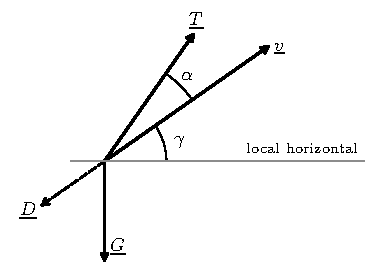
\includegraphics[width=0.36\linewidth]{losses}\end{center}
\begin{equation}
\frac{dv}{dt}=-\frac{\mu}{r^{2}}\,s_{\gamma}+\frac{T}{m}\,c_{\alpha}-\frac{D}{m}
=\frac{T}{m}-\frac{\mu}{r^{2}}\,s_{\gamma}-\frac{T}{m}\left(1-c_{\alpha}\right)-\frac{D}{m}.
\end{equation}
Integrating from $t_0$ to $t_f$:
\begin{equation}
\Delta v=\underbrace{\int_{t_0}^{t_f}\!\frac{T}{m}\,dt}_{\Delta v_T}
-\underbrace{\int_{t_0}^{t_f}\!\frac{\mu}{r^{2}}\,s_{\gamma}\,dt}_{\Delta v_G}
-\underbrace{\int_{t_0}^{t_f}\!\frac{T}{m}\left(1-c_{\alpha}\right)dt}_{\Delta v_M}
-\underbrace{\int_{t_0}^{t_f}\!\frac{D}{m}\,dt}_{\Delta v_D}.
\end{equation}

\paragraph{Physical meaning.}
\begin{itemize}
\item $\Delta v_T$ -- \textbf{ideal (Tsiolkovsky) velocity change}: since $T=-c\,\dot m$, $\Delta v_T=c\ln(m_0/m_f)$. It depends only
on the engine ($c$) and on the mass ratio, not on the trajectory.
\item $\Delta v_G$ -- \textbf{gravity loss}: the component of gravity along the velocity, $-g\,s_\gamma$, decelerates the vehicle
while it climbs (thrust spent to hold the vehicle up against gravity instead of accelerating it). It is large when the path is
steep ($\gamma$ near $90^\circ$) and the burn is long; it vanishes for horizontal flight.
\item $\Delta v_M$ -- \textbf{misalignment loss}: only the component $T c_\alpha$ changes the speed; the normal component
$T s_\alpha$ only rotates the velocity. It vanishes for $\alpha=0$ (gravity turn, thrust along $\underline v$).
\item $\Delta v_D$ -- \textbf{drag loss}: the work of the aerodynamic drag, which dissipates kinetic energy; it depends on
density, speed and on $S/m$ ($D/m=\frac12\rho v_R^2C_DS/m$).
\end{itemize}
All losses are positive integrals, so $\Delta v<\Delta v_T$. The equation holds for each sub-rocket.

\paragraph{Typical values and trends.} For VEGA: $\Delta v_T=3.054$, $\Delta v_G=0.683$, $\Delta v_M=0.019$, $\Delta v_D=0.107$\,km/s:
\textbf{gravity loss dominates}. In the early ascent $\gamma$ is large and $\Delta v_G$ dominates; a gravity-turn condition
($\alpha=0$) gives $\Delta v_M=0$; as velocity grows $D$ grows while $\gamma$ decreases, reducing $\Delta v_G$. Hence:
(a) the thick atmospheric layers are crossed along a \emph{near-radial} path, to limit drag and minimise the time spent in
them; (b) as soon as the density decreases the velocity is rotated to reduce $\gamma$, to avoid excessive gravity losses.

\begin{keyf}
$\dfrac{dv}{dt}=-\dfrac{\mu}{r^2}s_\gamma+\dfrac{T}{m}c_\alpha-\dfrac{D}{m}$; \
$\Delta v=\Delta v_T-\Delta v_G-\Delta v_M-\Delta v_D$; \ $\Delta v_T=\displaystyle\int\frac{T}{m}dt=c\ln\frac{m_0}{m_f}$, \
$\Delta v_G=\displaystyle\int\frac{\mu}{r^2}s_\gamma dt$, \ $\Delta v_M=\displaystyle\int\frac{T}{m}(1-c_\alpha)dt$, \ $\Delta v_D=\displaystyle\int\frac{D}{m}dt$.
\end{keyf}

\pitfalls
\begin{itemize}
\item Define $\gamma$ and $\alpha$ with a sketch; the gravity term has $s_\gamma$ (not $c_\gamma$) because $\gamma$ is measured from the horizontal.
\item The misalignment loss is $T(1-c_\alpha)/m$, not $T s_\alpha/m$.
\item Recall that $\Delta v_T$ is exactly Tsiolkovsky's $\Delta v$ and that the losses are always subtracted.
\end{itemize}

\source{cap06.tex l.112--162 (Tsiolkovsky's law), l.504--571 (losses equation, VEGA values, comments). Formulario: \fml{6-TSI}.}

% ---------------------------------------------------------------------
\question{A9}{Propulsive velocity and velocity losses in the ascent trajectory}
% source: cap06.tex l.356-502 (ascent phases), l.504-571 (losses)
\begin{qbox}
Define propulsive velocity and the velocity losses due to misalignment, gravity and aerodynamic effects in the ascent
trajectory of the launch vehicle. Explain how each type of velocity loss depends on vehicle trajectory and possibly other
launch vehicle features.
\qmeta{Jul 2025 (listed as a 2025 question).}
\qnote{Difference from \qref{A8}: same integrals; here the emphasis is on the dependence on the trajectory and the vehicle.}
\end{qbox}

\begin{outline}
\begin{enumerate}
\item Equation along $\hat v$ and the four integrals (sketch with $\gamma$, $\alpha$).
\item Propulsive (ideal) velocity $\Delta v_T=\int T/m\,dt=c\ln(m_0/m_f)$: engine and mass ratio only.
\item Gravity loss: depends on $\gamma(t)$ and burn time $\Rightarrow$ thrust-to-weight ratio, steepness of the path.
\item Misalignment loss: depends on $\alpha(t)$ $\Rightarrow$ gravity turn, structural limit $q\alpha$.
\item Drag loss: depends on $\rho(h)$, $v$, ballistic coefficient $C_DS/m$ $\Rightarrow$ fast near-vertical crossing.
\item Trade-off steep vs shallow ascent; phases of the ascent; VEGA numbers.
\end{enumerate}
\end{outline}

\answer
\paragraph{Losses equation.} Projecting $\dot{\underline v}=(\underline G+\underline A+\underline T)/m$ on the velocity direction
($\gamma$ = flight-path angle from the local horizontal, $\alpha$ = angle between thrust and velocity, $D$ = drag):
\begin{equation}
\frac{dv}{dt}=\frac{T}{m}-\frac{\mu}{r^{2}}\,s_{\gamma}-\frac{T}{m}\left(1-c_{\alpha}\right)-\frac{D}{m}
\;\Rightarrow\;
\Delta v=\Delta v_T-\Delta v_G-\Delta v_M-\Delta v_D .
\end{equation}
\begin{center}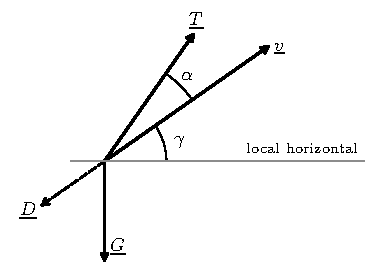
\includegraphics[width=0.33\linewidth]{losses}\end{center}

\paragraph{Propulsive velocity.} The propulsive (ideal) velocity is the velocity change that the thrust alone would produce:
\begin{equation}
\Delta v_T=\int_{t_0}^{t_f}\frac{T}{m}\,dt=\int_{t_0}^{t_f}-c\frac{\dot m}{m}\,dt=c\ln\frac{m_0}{m_f}\qquad(c=g_0I_{sp}).
\end{equation}
It coincides with Tsiolkovsky's $\Delta v$; it depends only on the engine (effective exhaust velocity) and on the mass
ratio of the stage, \emph{not} on the trajectory. The actual gain is $\Delta v_T$ minus the three losses.

\paragraph{Gravity loss} $\Delta v_G=\displaystyle\int\frac{\mu}{r^2}s_\gamma\,dt$.
\begin{itemize}
\item \emph{Trajectory}: proportional to $s_\gamma$: maximum during the vertical arc ($\gamma=90^\circ$), small when the path is
nearly horizontal. Early pitch-over / lower $\gamma$ reduce it.
\item \emph{Vehicle}: it is an integral over time, so it grows with the \emph{burn duration}: a high thrust-to-weight ratio
(short burns) reduces it, a low-thrust upper stage that burns long while climbing increases it.
\item Usually the largest loss (VEGA: 0.683\,km/s out of 3.054).
\end{itemize}

\paragraph{Misalignment loss} $\Delta v_M=\displaystyle\int\frac{T}{m}(1-c_\alpha)\,dt$.
\begin{itemize}
\item \emph{Trajectory/steering}: zero when the thrust is aligned with the velocity ($\alpha=0$), as in the \textbf{gravity turn}, where
gravity alone turns the velocity. It appears in the pitch manoeuvre and in the rarefied-atmosphere arcs where an incidence is used
to shape the trajectory.
\item \emph{Vehicle}: the admissible $\alpha$ is limited by structural loads, $q\alpha\le(q\alpha)_{\max}$ with $q=\frac12\rho v_R^2$; vehicles
that tolerate an incidence (military-derived) can steer more but pay this loss. It is the smallest (VEGA: 0.019\,km/s).
\end{itemize}

\paragraph{Drag loss} $\Delta v_D=\displaystyle\int\frac{D}{m}\,dt$, \quad $\dfrac{D}{m}=\dfrac12\rho v_R^2\,C_D\dfrac{S}{m}$.
\begin{itemize}
\item \emph{Trajectory}: depends on the density along the path ($\rho$ decreases exponentially with altitude) and on the speed:
the dense layers (below $\sim40$\,km) must be crossed \emph{quickly and near-vertically}, before reaching high speeds.
\item \emph{Vehicle}: proportional to the ballistic coefficient $C_DS/m$ (shape, cross-section, mass); large, heavy vehicles have
smaller $S/m$ and hence smaller drag losses \notinnotes. VEGA: 0.107\,km/s.
\end{itemize}

\paragraph{Trade-off and ascent phases.} A steep path reduces drag losses but increases gravity losses; a shallow path does the
opposite. Real ascents: vertical arc at launch (launch-site safety; avoid premature rotation of $\underline v$), roll and pitch
manoeuvres (select the orbit plane; some misalignment), \textbf{gravity turn} ($\alpha=0$ to avoid destructive bending loads:
$\Delta v_M\approx0$), rarefied-atmosphere arc (small $\alpha$ allowed), coast arc, injection arc (thrust nearly horizontal:
$\Delta v_G\approx0$). Hence: near-radial crossing of the thick atmosphere, then rotation of $\underline v$ to reduce $\gamma$.

\begin{keyf}
$\Delta v_T=\displaystyle\int\frac Tm dt=c\ln\frac{m_0}{m_f}$; \ $\Delta v_G=\displaystyle\int g\,s_\gamma dt$ (steepness, burn time);
\ $\Delta v_M=\displaystyle\int\frac Tm(1-c_\alpha)dt$ (steering, $q\alpha$ limit); \ $\Delta v_D=\displaystyle\int\frac12\rho v^2C_D\frac{S}{m}dt$ (density, speed, $C_DS/m$).
\end{keyf}

\pitfalls
\begin{itemize}
\item "Propulsive velocity" is the ideal $\Delta v_T$, not the final orbital speed.
\item For each loss say both the trajectory dependence and a vehicle feature (thrust-to-weight, structural $q\alpha$ limit, $C_DS/m$).
\item Mention the conflicting requirements (drag vs gravity) and the gravity turn.
\end{itemize}

\source{cap06.tex l.356--482 (phases of the ascent), l.504--571 (losses). Formulario: \fml{6-TSI}.}

% ---------------------------------------------------------------------
\question{A10}{Rocket staging: mass-distribution parameters and motivation}
% source: cap06.tex l.164-224, 225-354
\begin{qbox}
With regard to rocket staging, define the key mass-distribution parameters of each stage and briefly justify the use of
staging for launch vehicles.
\qmeta{list by chapter (Ch.\,6).}
\qnote{Adjacent to \qref{A11} (same parameters; A11 asks for the total $\Delta V$ formula).}
\end{qbox}

\begin{outline}
\begin{enumerate}
\item Sub-rocket $i$: $m_0^{(i)}=m_s^{(i)}+m_p^{(i)}+m_u^{(i)}$, $m_u^{(i)}=m_0^{(i+1)}$ (sketch).
\item Structural coefficient $\epsilon_s^{(i)}$ (technology, $\ge\epsilon_{s,\min}$) and mass ratio $u_0^{(i)}=m_f^{(i)}/m_0^{(i)}$.
\item Masses in terms of $(\epsilon_s,u_0)$; $\Delta v^{(i)}=-c_i\ln u_0^{(i)}$; $m_u>0$ iff $u_0>\epsilon_s$; low $\epsilon_s$ desirable.
\item Why staging: discard useless structural mass; single-stage limit $c\ln(1/\epsilon_s)$; $\Delta v_{\max}(N)$ with diminishing returns, 3--4 stages.
\end{enumerate}
\end{outline}

\answer
\paragraph{Definitions.} A multistage launch vehicle is a sequence of sub-rockets. Sub-rocket $i$ has initial mass
\begin{equation}
m_{0}^{(i)}=m_{s}^{(i)}+m_{p}^{(i)}+m_{u}^{(i)},
\end{equation}
$m_s^{(i)}$ = structural (inert) mass of stage $i$ (tanks, engines, structure), $m_p^{(i)}$ = propellant mass,
$m_u^{(i)}$ = "payload" of sub-rocket $i$, i.e.\ the initial mass of the next sub-rocket, $m_u^{(i)}=m_0^{(i+1)}$, and the true
payload for the last one.
\begin{center}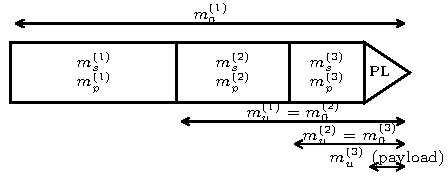
\includegraphics[width=0.7\linewidth]{staging}\end{center}
The mass distribution of each stage is described by two parameters:
\begin{equation}
\epsilon_{s}^{(i)}=\frac{m_{s}^{(i)}}{m_{s}^{(i)}+m_{p}^{(i)}}\quad\text{(structural coefficient)},\qquad
u_{0}^{(i)}=\frac{m_{f}^{(i)}}{m_{0}^{(i)}}=\frac{m_{s}^{(i)}+m_{u}^{(i)}}{m_{0}^{(i)}}\quad\text{(mass ratio)}.
\end{equation}
$\epsilon_s$ depends on the \textbf{technology} (materials, tank pressure, engine mass), so $\epsilon_s^{(i)}\ge\epsilon_{s,\min}^{(i)}$;
$u_0$ is the final-to-initial mass ratio of the burn. Inverting the definitions:
\begin{equation}
m_{p}^{(i)}=m_{0}^{(i)}\left[1-u_{0}^{(i)}\right],\quad
m_{s}^{(i)}=m_{0}^{(i)}\frac{\epsilon_{s}^{(i)}\left[1-u_{0}^{(i)}\right]}{1-\epsilon_{s}^{(i)}},\quad
m_{u}^{(i)}=m_{0}^{(i)}\frac{u_{0}^{(i)}-\epsilon_{s}^{(i)}}{1-\epsilon_{s}^{(i)}},
\end{equation}
and the velocity change of stage $i$ (Tsiolkovsky) is $\Delta v^{(i)}=-c_i\ln u_0^{(i)}$.
\begin{itemize}
\item $m_u^{(i)}>0$ only if $u_0^{(i)}>\epsilon_s^{(i)}$; for $u_0=\epsilon_s$ the stage carries nothing.
\item At given $u_0$ (i.e.\ given $\Delta v^{(i)}$) the payload fraction $m_u/m_0$ is maximum for $\epsilon_s=\epsilon_{s,\min}$:
\textbf{low structural coefficients} improve performance.
\end{itemize}

\paragraph{Why staging.} The purpose is to increase the overall $\Delta v$ by \textbf{discarding structural masses that have become
useless} (empty tanks and their engines). With a single stage the whole structure must be accelerated up to the final speed;
even with zero payload ($u_0\to\epsilon_s$) the maximum is
\begin{equation}
\Delta v_{\max}^{\text{single}}=c\ln\frac{1}{\epsilon_s},
\end{equation}
e.g.\ $c=3$\,km/s, $\epsilon_s=0.1$ $\Rightarrow$ 6.9\,km/s, below the $\approx9$--10\,km/s needed to reach LEO including
losses \notinnotes. With $N$ stages the velocity changes add up, $\Delta v=-\sum_i c_i\ln u_0^{(i)}$; for similar stages the optimal
distribution (all $u_0^{(i)}$ equal) gives
\begin{equation}
\Delta v_{\max}=-c\,N\ln\left\{\epsilon_{s}+(1-\epsilon_{s})\left[\frac{m_{u}^{(N)}}{m_{0}^{(1)}}\right]^{1/N}\right\},
\end{equation}
which increases with $N$ with diminishing returns and has a finite limit for $N\to\infty$. Structural and operational complexity
grow with $N$: launch vehicles rarely have more than 5 stages (often 3--4). Staging also allows engines optimised for
different altitudes (sea-level vs vacuum nozzles) \notinnotes.

\begin{keyf}
$m_0^{(i)}=m_s^{(i)}+m_p^{(i)}+m_u^{(i)}$, \ $\epsilon_s=\dfrac{m_s}{m_s+m_p}$, \ $u_0=\dfrac{m_s+m_u}{m_0}$, \
$\dfrac{m_u}{m_0}=\dfrac{u_0-\epsilon_s}{1-\epsilon_s}$, \ $\Delta v^{(i)}=-c_i\ln u_0^{(i)}$.
\end{keyf}

\pitfalls
\begin{itemize}
\item $\epsilon_s$ uses structure + propellant only (no payload); $u_0$ uses the final mass, which includes the upper stages.
\item The "payload" of stage $i$ is the whole upper composite, $m_u^{(i)}=m_0^{(i+1)}$.
\item Justify staging with the single-stage limit and the diminishing returns with $N$.
\end{itemize}

\source{cap06.tex l.164--224 (rocket staging), l.225--354 (optimal staging, plot of $\Delta v_{\max}$ vs $N$; source errata \#5--6). Formulario: \fml{6-STG}, \fml{6-STM}, \fml{6-OPT}.}

% ---------------------------------------------------------------------
\question{A11}{Tsiolkovsky's law and the $\Delta V$ of a multistage rocket}
% source: cap06.tex l.21-110 (thrust, c, Isp), l.112-162 (Tsiolkovsky), l.164-354 (staging)
\begin{qbox}
State Tsiolkovsky's law and use it to evaluate the total $\Delta V$ of a multiple-stage rocket in terms of its propellant, inert,
and payload mass. Define the structural coefficient and specific impulse and discuss their effect on the total $\Delta V$.
\qmeta{Sep 2025 (listed as a 2025 question).}
\qnote{Adjacent to \qref{A10} (parameters of each stage) and \qref{A8} (losses with respect to this ideal law).}
\end{qbox}

\begin{outline}
\begin{enumerate}
\item Thrust and effective exhaust velocity $c=g_0I_{sp}$; $\dot m=-T/c$.
\item Assumptions; derivation $\dot v=-c\dot m/m$ $\Rightarrow$ $\Delta v=c\ln(m_0/m_f)$, $m_f=m_0e^{-\Delta v/c}$; meaning (upper bound).
\item Multistage: masses of each stage, $m_0^{(i)}$ and $m_f^{(i)}$ in terms of $m_p$, $m_s$, $m_{PL}$; $\Delta v_{tot}=\sum c_i\ln(m_0^{(i)}/m_f^{(i)})$.
\item Structural coefficient $\epsilon_s$ and specific impulse $I_{sp}$: definitions and effect on $\Delta v_{tot}$.
\end{enumerate}
\end{outline}

\answer
\paragraph{Thrust and specific impulse.} From the momentum balance of the vehicle and of the ejected mass,
$\underline T=\dot m\,\underline c_{ej}+A_e(p_e-p_a)\hat v=-\dot m\,(-\underline c)$, i.e.\ $T=|\dot m|\,c$, with the
\emph{effective exhaust velocity} $\underline c=\underline c_{ej}+A_e(p_e-p_a)\hat v/\dot m$ (includes the pressure thrust), and
\begin{equation}
\dot m=-\frac{T}{c},\qquad c=g_0I_{sp}.
\end{equation}
The \textbf{specific impulse} $I_{sp}$ [s] is the effective exhaust velocity divided by $g_0$ (sea-level gravity): the impulse
delivered per unit weight of propellant consumed. Typical: solid $\sim$270--290\,s, LOX/LH$_2$ $\sim$450\,s \notinnotes.

\paragraph{Tsiolkovsky's law.} Assumptions: no aerodynamic force, no gravity, thrust aligned with the velocity (valid for
impulsive manoeuvres or motion without $\underline G$ and $\underline A$). Then
\begin{equation}
\sys{\frac{dv}{dt}&=\frac{T}{m}\\ \dot m&=-\frac{T}{c}}\;\Rightarrow\;\dot v=-c\,\frac{\dot m}{m}
\;\Rightarrow\;\Delta v=v_f-v_0=c\ln\frac{m_0}{m_f},\qquad m_f=m_0\,e^{-\Delta v/c}.
\end{equation}
It relates the propellant consumption $m_p=m_0-m_f$ to the velocity change; it gives the \emph{maximum} $\Delta v$ for a given
mass ratio (minimum propellant for a given $\Delta v$): real ascents suffer gravity, drag and misalignment losses.

\paragraph{Multistage rocket.} Stage $j$ ($j=1\dots N$, burnt in this order) has propellant $m_p^{(j)}$ and inert mass $m_s^{(j)}$; the
payload is $m_{PL}$. Stage $i$ burns while all upper stages and the payload are attached and the lower stages have been jettisoned:
\begin{equation}
m_0^{(i)}=m_{PL}+\sum_{j=i}^{N}\left(m_s^{(j)}+m_p^{(j)}\right),\qquad m_f^{(i)}=m_0^{(i)}-m_p^{(i)},
\end{equation}
\begin{equation}
\boxed{\;\Delta v_{tot}=\sum_{i=1}^{N}c_i\ln\frac{m_0^{(i)}}{m_f^{(i)}}
=\sum_{i=1}^{N}g_0I_{sp}^{(i)}\ln\frac{m_{PL}+\sum_{j=i}^{N}\left(m_s^{(j)}+m_p^{(j)}\right)}{m_{PL}+m_s^{(i)}+\sum_{j=i+1}^{N}\left(m_s^{(j)}+m_p^{(j)}\right)}\;}
\end{equation}
In the notation of the notes, $m_u^{(i)}=m_0^{(i+1)}$, $u_0^{(i)}=m_f^{(i)}/m_0^{(i)}$ and $\Delta v_{tot}=-\sum_ic_i\ln u_0^{(i)}$.
The dropped inert mass $m_s^{(i)}$ is no longer accelerated by the upper stages: this is the gain of staging.

\paragraph{Structural coefficient and its effect.} $\epsilon_s^{(i)}=\dfrac{m_s^{(i)}}{m_s^{(i)}+m_p^{(i)}}$ (fraction of inert mass in
the stage; set by technology, $\epsilon_s\ge\epsilon_{s,\min}$). Since $u_0^{(i)}=\epsilon_s^{(i)}+(1-\epsilon_s^{(i)})\,m_u^{(i)}/m_0^{(i)}$, at
given payload fractions a smaller $\epsilon_s$ gives a smaller $u_0$ and a larger $\Delta v$; at given $\Delta v$, it gives a larger payload.
Each stage is limited by $\Delta v^{(i)}<c_i\ln(1/\epsilon_s^{(i)})$, and for similar optimal stages
$\Delta v_{\max}=-cN\ln\{\epsilon_s+(1-\epsilon_s)[m_u^{(N)}/m_0^{(1)}]^{1/N}\}$ decreases as $\epsilon_s$ increases.

\paragraph{Specific impulse and its effect.} $\Delta v$ is \emph{proportional} to $c=g_0I_{sp}$: at given masses, $\Delta v$ scales linearly
with $I_{sp}$ ($\partial\Delta v^{(i)}/\partial c_i=\ln(m_0^{(i)}/m_f^{(i)})$); at given $\Delta v$ the propellant fraction
$1-e^{-\Delta v/c}$ decreases exponentially with $I_{sp}$. High-$I_{sp}$ engines are therefore most valuable on the upper stages,
whose mass ratio multiplies the whole payload \notinnotes.

\begin{keyf}
$c=g_0I_{sp}$, $\dot m=-T/c$; \ $\Delta v=c\ln\dfrac{m_0}{m_f}$; \ $\Delta v_{tot}=\displaystyle\sum_i c_i\ln\frac{m_0^{(i)}}{m_0^{(i)}-m_p^{(i)}}$,
$m_0^{(i)}=m_{PL}+\displaystyle\sum_{j\ge i}(m_s^{(j)}+m_p^{(j)})$; \ $\epsilon_s=\dfrac{m_s}{m_s+m_p}$.
\end{keyf}

\pitfalls
\begin{itemize}
\item In stage $i$ the initial mass includes all upper stages and the payload, but not the jettisoned lower stages.
\item State the three assumptions of Tsiolkovsky's law and that it gives an upper bound.
\item $I_{sp}$ in seconds: multiply by $g_0=9.80665$\,m/s$^2$.
\end{itemize}

\source{cap06.tex l.21--110 (thrust, $c$, $I_{sp}$), l.112--162 (Tsiolkovsky), l.164--224 (staging parameters), l.225--354 (optimal staging).
Formulario: \fml{6-ISP}, \fml{6-TSI}, \fml{6-DVN}.}

% =====================================================================
% Group B -- Chapter 5: orbital motion in multibody environments (one question per exam)
% Source: latex_notes/SFM_05_Orbital Motion in Multibody Environments/cap05.tex
% =====================================================================
\qgroup{B}{Chapter 5 -- Multibody environments and the CR3BP}

One of the three orbital-mechanics questions is always on Chapter 5. Notation of the notes: primaries $m_1>m_2$, mass
parameter $\mu=m_2/(m_1+m_2)$, synodic coordinates $(x,y,z)$, angular velocity $\omega$ of the primaries ($\omega=1$\,TU$^{-1}$
in canonical units, as in the exam texts). Earth--Moon: $\mu=1/82.27=0.01216$.

\begin{center}
\small
\begin{tabular}{@{}lllr@{}}
\toprule
Q & Topic & Asked & Page\\
\midrule
\ref{q:B1} & Jacobi interval, Earth--Moon transfers without escape & $\times$2, Jan 2023, Jul 2025 & \pageref{q:B1}\\
\ref{q:B2} & Synodic frame, 5 libration points, ZVC with/without escape & $\times$2, Feb 2025 & \pageref{q:B2}\\
\ref{q:B3} & Collinear libration points: equation for their position & list & \pageref{q:B3}\\
\ref{q:B4} & Proof of the Jacobi integral & $\times$2, Sep 2024, Jan 2025, Mar 2025 & \pageref{q:B4}\\
\ref{q:B5} & Synodic frame: primaries and their $\mu$-dependence & list & \pageref{q:B5}\\
\ref{q:B6} & $N$-body integrals, Laplace plane, $\underline H_c$ conserved & $\times$2, Jun 2025, Sep 2025 & \pageref{q:B6}\\
\bottomrule
\end{tabular}
\end{center}

Common data used in this group (computed from $\Omega$ with $\mu=1/82.27$, $\omega=1$):
\begin{center}
\small
\begin{tabular}{@{}lccccc@{}}
\toprule
 & $L_1$ & $L_2$ & $L_3$ & $L_{4,5}$\\
\midrule
$x$ [DU] & $0.8369$ & $1.1557$ & $-1.0051$ & $0.5-\mu$, $y=\pm\sqrt3/2$\\
$C_i=2\Omega(L_i)$ & $3.18838$ & $3.17220$ & $3.01215$ & $2.98799$\\
\bottomrule
\end{tabular}
\end{center}
{\footnotesize ($C_1$ in the notes reads 3.18338: typo corrected, errata \#20.) DU $=R=384400$\,km, TU $=1/\omega\simeq4.34$\,days.}

% ---------------------------------------------------------------------
\question{B1}{Earth--Moon CR3BP: Jacobi interval for transfers without escape}
% source: cap05.tex l.379-467 (Jacobi integral, ZVS), l.469-571 (libration points, Omega at Li), l.573-613 (special values of C)
\begin{qbox}
In the circular restricted three-body problem (CR3BP) with Earth and Moon as primaries, identify the Jacobi-integral
interval that allows Earth--Moon transfers without any possible escape toward the outer space, referencing the
zero-velocity curves. Depict the curve geometry.
\qmeta{$\times$2 in the list (2025); Jan 2023; Jul 2025 ("provide the definition of the Jacobi integral").}
\qnote{Difference from \qref{B2}: B2 also asks for the synodic frame, the five libration points and the case \emph{with} an
escape route.}
\end{qbox}

\begin{outline}
\begin{enumerate}
\item CR3BP hypotheses; synodic frame; potential $\Omega$; equations $\ddot x-2\omega\dot y=\Omega_x$, \dots
\item Jacobi integral $C=2\Omega-(\dot x^2+\dot y^2+\dot z^2)$ (one-line proof); $C$ decreases as energy increases.
\item Zero-velocity surfaces/curves: $v^2=2\Omega-C\ge0$ defines the Hill region; shape (spheres near primaries, cylinder far away).
\item Libration points and $C_i=2\Omega(L_i)$: $C_1>C_2>C_3>C_{4,5}$; Earth--Moon values.
\item Answer: $C_2<C<C_1$: the neck at $L_1$ is open (Earth--Moon transfer), the neck at $L_2$ closed (no escape). Sketch.
\end{enumerate}
\end{outline}

\answer
\paragraph{Model.} The CR3BP studies a third body (spacecraft) of negligible mass, $m\ll m_2<m_1$, attracted by two
\emph{primaries} (Earth and Moon) that move on circular orbits about their centre of mass with angular velocity
$\omega=\sqrt{G(m_1+m_2)/R^3}$; the spacecraft does not affect the primaries. In the \textbf{synodic frame} (origin at the centre of
mass, $\hat\imath$ from $m_1$ towards $m_2$, $\hat k$ along the angular momentum of the primaries, rotating with $\omega$) the primaries are
fixed at $x_1=-\mu$, $x_2=1-\mu$ (DU $=R$, TU $=1/\omega$), and the motion obeys
\begin{equation}
\ddot{x}-2\omega\dot{y}=\frac{\partial\Omega}{\partial x},\qquad
\ddot{y}+2\omega\dot{x}=\frac{\partial\Omega}{\partial y},\qquad
\ddot{z}=\frac{\partial\Omega}{\partial z},
\end{equation}
\begin{equation}
\Omega=\frac{\omega^{2}}{2}(x^{2}+y^{2})+\frac{1-\mu}{r_1}+\frac{\mu}{r_2},\qquad
r_1=\sqrt{(x+\mu)^{2}+y^{2}+z^{2}},\ \ r_2=\sqrt{(x+\mu-1)^{2}+y^{2}+z^{2}} .
\end{equation}

\paragraph{Jacobi integral (definition).} Multiplying the three equations by $\dot x$, $\dot y$, $\dot z$ and adding, the Coriolis terms
cancel and, since $\Omega$ depends only on the position, $\frac12\frac{d}{dt}(\dot x^2+\dot y^2+\dot z^2)=\frac{d\Omega}{dt}$. Hence
\begin{equation}
C:=2\Omega(x,y,z)-\left(\dot{x}^{2}+\dot{y}^{2}+\dot{z}^{2}\right)=\text{const}
\end{equation}
is an integral of motion of the CR3BP, fixed by the initial conditions. It is related to the energy: \textbf{$C$ decreases as the
mechanical energy increases} (a $\Delta v$ that increases the speed lowers $C$).

\paragraph{Zero-velocity surfaces and curves.} Since $v^2=2\Omega(x,y,z)-C\ge0$, motion is possible only where $2\Omega\ge C$
(\emph{Hill's region}). The boundary $2\Omega=C$, where the velocity would be zero, is the zero-velocity surface (curve in the
$x$--$y$ plane). For large $x,y$ the term $\omega^2(x^2+y^2)$ dominates (near-cylinder about $z$); close to a primary the
corresponding $1/r_i$ term dominates (near-sphere around $m_1$ or $m_2$). For large $C$ (low energy) motion is confined
inside the spheres or outside the cylinder; as $C$ decreases the regions grow and \textbf{merge through "necks" located at the
libration points}.

\paragraph{Critical values of $C$.} At a libration point $L_i$ (equilibrium in the synodic frame) the velocity is zero, so $L_i$
lies on the zero-velocity curve with $C_i=2\Omega(L_i)$. For Earth--Moon:
$C_1=3.18838>C_2=3.17220>C_3=3.01215>C_{4,5}=2.98799$ (canonical units). The topology changes exactly at these values:
\begin{itemize}
\item $C>C_1$: three separate regions (around the Earth, around the Moon, outside): no transfer possible;
\item $C_2<C<C_1$: the neck at $L_1$ opens;
\item $C_3<C<C_2$: also the neck at $L_2$ opens (escape);
\item $C_{4,5}<C<C_3$: forbidden only near $L_4$, $L_5$; \quad $C<C_{4,5}$: motion allowed everywhere.
\end{itemize}

\paragraph{Answer: Earth--Moon transfers without escape.}
\begin{equation}
\boxed{\;C_2<C<C_1\qquad(3.17220<C<3.18838\ \text{for Earth--Moon})\;}
\end{equation}
The inner zero-velocity curve has an opening at $L_1$, between Earth and Moon: an \emph{interior transfer} from the region around
the Earth to the region around the Moon is feasible, passing close to $L_1$. The opening at $L_2$ (behind the Moon) is still closed:
the inner region (Earth + Moon) is separated by a forbidden ring from the exterior region, so \textbf{no escape} toward outer space is
possible. Motion outside the outer curve is also allowed, but it cannot be reached from the inner region.

\begin{center}
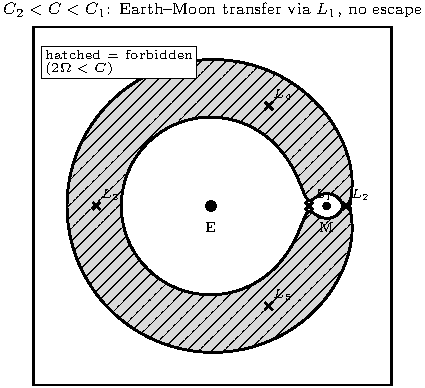
\includegraphics[width=0.48\linewidth]{zvc_noescape}\hfill
\begin{minipage}[b]{0.48\linewidth}\small
Computed with $\mu=1/82.27$ and $C=(C_1+C_2)/2$. Hatched: forbidden region ($2\Omega<C$).
The white region around E and M is connected through the $L_1$ neck;
the hatched ring is closed at $L_2$, so the exterior (white, outside) is unreachable.\\[4pt]
Lowering $C$ (more energy, e.g.\ a larger injection $\Delta v$) widens the $L_1$ neck; at $C=C_2$ the $L_2$ neck opens and escape
becomes possible.
\end{minipage}
\end{center}

\begin{fig2draw}
E (big dot) and M (small dot) on the $x$-axis. Draw a closed curve around the Earth and a small one around the Moon touching
it at $L_1$ (between them, slightly open: a "peanut" with a neck), and a large closed oval outside both, closed near $L_2$.
Hatch the ring between the inner peanut and the outer oval. Write $C_2<C<C_1$.
\end{fig2draw}

\begin{keyf}
$C=2\Omega-(\dot x^2+\dot y^2+\dot z^2)$, \ $\Omega=\frac{\omega^2}{2}(x^2+y^2)+\frac{1-\mu}{r_1}+\frac{\mu}{r_2}$, \
Hill region $2\Omega\ge C$, \ $C_i=2\Omega(L_i)$, \ $C_1>C_2>C_3>C_{4,5}$, \ no-escape transfer: $C_2<C<C_1$.
\end{keyf}

\pitfalls
\begin{itemize}
\item Higher $C$ means \emph{lower} energy: the order of the intervals is reversed with respect to the energy.
\item "Without escape" requires the $L_2$ neck closed (lower bound $C_2$) and "transfer" requires the $L_1$ neck open (upper bound $C_1$).
\item The forbidden region is where $2\Omega<C$; hatch it clearly and mark $L_1$, $L_2$.
\end{itemize}

\source{cap05.tex l.244--305 (CR3BP, synodic frame), l.307--413 (equations, Jacobi integral), l.415--467 (zero-velocity surfaces),
l.573--613 (special values of $C$, Earth--Moon values). Figure computed in \texttt{figures/src/make\_figures.py}.}

% ---------------------------------------------------------------------
\question{B2}{Synodic frame, the five libration points, zero-velocity curves with and without escape}
% source: cap05.tex l.259-305, 469-535, 573-613
\begin{qbox}
In the CR3BP, plot the five libration points in the synodic frame and define that frame. Then, for Earth--Moon primaries,
draw the zero-velocity curves that allow Earth-to-Moon transfers without escape; also show the case where an escape route
exists, and state the corresponding Jacobi-constant interval.
\qmeta{$\times$2 in the list (2025); Feb 2025 ("draw the case with a single escape route outward and define the interval of $C$").}
\qnote{Difference from \qref{B1}: adds the synodic frame, the libration points and the escape case.}
\end{qbox}

\begin{outline}
\begin{enumerate}
\item Synodic frame: origin at the centre of mass, $\hat\imath$ towards $m_2$, $\hat k\parallel\underline H$, rotating with $\omega$; canonical units; primaries at $-\mu$, $1-\mu$.
\item Libration points: equilibria with zero velocity, $\Omega_x=\Omega_y=0$; three collinear ($L_3<x_1<L_1<x_2<L_2$) and two triangular ($r_1=r_2=1$). Sketch.
\item Jacobi integral and Hill region $2\Omega\ge C$; $C_i=2\Omega(L_i)$, $C_1>C_2>C_3>C_{4,5}$.
\item No escape: $C_2<C<C_1$ (sketch). Single escape route: $C_3<C<C_2$, exit through $L_2$ (sketch).
\item Complete list of the five regimes.
\end{enumerate}
\end{outline}

\answer
\paragraph{Synodic frame.} Two primaries $m_1>m_2$ move on circular orbits about their centre of mass $O'$ with constant
distance $R$ and angular velocity $\omega=\sqrt{G(m_1+m_2)/R^3}$. The synodic frame $\{\hat\imath,\hat\jmath,\hat k\}$ has origin in
$O'$, $\hat\imath$ along the line of the primaries (from $m_1$ to $m_2$), $\hat k$ parallel to their angular momentum
$\underline H$, $\hat\jmath=\hat k\times\hat\imath$, and \textbf{rotates with the primaries}: with respect to the inertial axes
$\{\hat c_1,\hat c_2,\hat c_3\}$ (coincident at $t=0$)
\begin{equation}
\begin{bmatrix}\hat\imath\\ \hat\jmath\\ \hat k\end{bmatrix}=
\begin{bmatrix}\cos\omega t&\sin\omega t&0\\-\sin\omega t&\cos\omega t&0\\0&0&1\end{bmatrix}
\begin{bmatrix}\hat c_1\\ \hat c_2\\ \hat c_3\end{bmatrix}.
\end{equation}
In canonical units (DU $=R$, TU $=1/\omega$, so $G(m_1+m_2)=1$) the primaries are \emph{fixed} at $x_1=-\mu$, $x_2=1-\mu$,
with $\mu=m_2/(m_1+m_2)<1/2$. The spacecraft position is $\underline r=x\hat\imath+y\hat\jmath+z\hat k$ and its equations of motion
are $\ddot x-2\omega\dot y=\Omega_x$, $\ddot y+2\omega\dot x=\Omega_y$, $\ddot z=\Omega_z$ with
$\Omega=\frac{\omega^2}{2}(x^2+y^2)+\frac{1-\mu}{r_1}+\frac{\mu}{r_2}$.

\paragraph{Libration (Lagrange) points.} Equilibrium points in the synodic frame, where the spacecraft can stay indefinitely if
placed with zero velocity. They lie in the $x$--$y$ plane and require $\dot x=\dot y=\ddot x=\ddot y=0$, i.e.\ $\Omega_x=\Omega_y=0$:
\begin{itemize}
\item \textbf{collinear points} ($y=0$): one root of a quintic in each interval: $L_3$ ($x<-\mu$, beyond $m_1$), $L_1$ (between the
primaries), $L_2$ (beyond $m_2$) -- see \qref{B3};
\item \textbf{triangular points} ($y\neq0$): $r_1=r_2=1$ DU, i.e.\ $L_4$, $L_5$ form \textbf{equilateral triangles} with the primaries
($x=\frac12-\mu$, $y=\pm\frac{\sqrt3}{2}$), above and below the $x$-axis, for any $\mu$.
\end{itemize}
\begin{center}
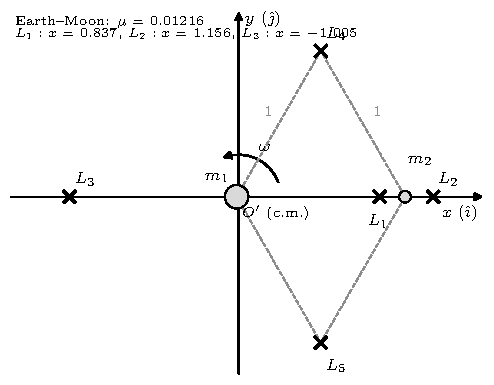
\includegraphics[width=0.5\linewidth]{lagrange}\hfill
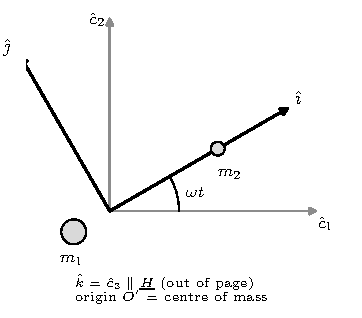
\includegraphics[width=0.36\linewidth]{synodic}
\end{center}
$\Omega$ is stationary at every $L_i$: only stationary (saddle) at $L_{1,2,3}$, a minimum at $L_{4,5}$ with
$2\Omega_{\min}=3-\mu(1-\mu)$.

\paragraph{Zero-velocity curves.} The Jacobi integral $C=2\Omega-v^2$ is constant; motion is allowed only where $2\Omega\ge C$.
At $L_i$ the velocity is zero, so the curve through $L_i$ corresponds to $C_i=2\Omega(L_i)$, with
$C_1>C_2>C_3>C_{4,5}$ (Earth--Moon: 3.18838, 3.17220, 3.01215, 2.98799).

\paragraph{The two requested cases.}
\begin{center}
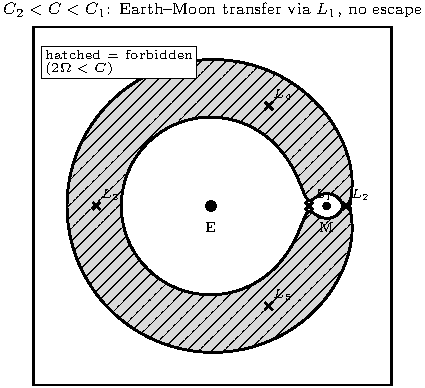
\includegraphics[width=0.46\linewidth]{zvc_noescape}\hfill
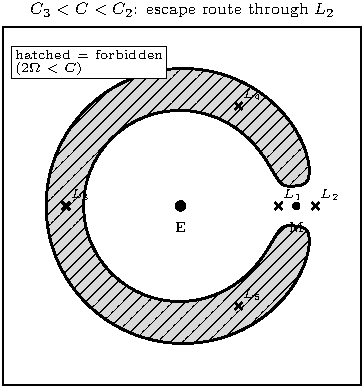
\includegraphics[width=0.46\linewidth]{zvc_escape}
\end{center}
\begin{itemize}
\item \textbf{Earth--Moon transfer, no escape}: $\boxed{C_2<C<C_1}$. The neck at $L_1$ is open (interior transfer Earth $\leftrightarrow$
Moon close to $L_1$), the neck at $L_2$ is closed: the forbidden ring separates the Earth--Moon region from outer space.
\item \textbf{Single escape route}: $\boxed{C_3<C<C_2}$. Both necks $L_1$ and $L_2$ are open: interior transfers (through $L_1$) and
exterior transfers (through $L_2$) are feasible, and a spacecraft can leave the Earth--Moon system \emph{only} through the opening
behind the Moon at $L_2$; the forbidden region becomes a horseshoe, still closed at $L_3$.
\end{itemize}

\paragraph{All regimes} (as $C$ decreases, i.e.\ energy increases):
\begin{enumerate}[label=(\arabic*)]
\item $C<C_{4,5}$: motion allowed in the entire space (no zero-velocity curve);
\item $C_{4,5}<C<C_3$: motion forbidden only near $L_4$ and $L_5$;
\item $C_3<C<C_2$: interior (via $L_1$) and exterior (via $L_2$) transfers;
\item $C_2<C<C_1$: interior transfers only; outside motion feasible but not reachable;
\item $C>C_1$: no transfer: confined near $m_1$, near $m_2$, or outside.
\end{enumerate}
\begin{center}
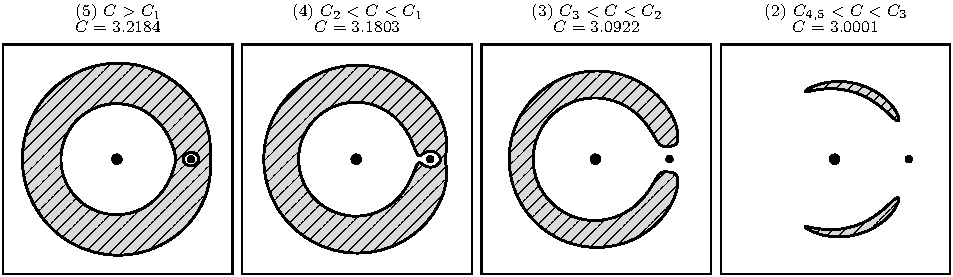
\includegraphics[width=0.95\linewidth]{zvc_cases}
\end{center}

\begin{fig2draw}
Axes $x,y$; E at $-\mu$ (left of $O'$, almost on it), M at $1-\mu$; $L_1$ between them close to the Moon, $L_2$ just beyond the Moon,
$L_3$ at $x\approx-1$, $L_4$/$L_5$ at the vertices of the equilateral triangles. Then two sketches: hatched ring closed at
$L_2$ ($C_2<C<C_1$) and hatched horseshoe open at $L_2$ ($C_3<C<C_2$).
\end{fig2draw}

\begin{keyf}
Synodic: origin c.m., $\hat\imath$ $m_1\!\to\! m_2$, $\hat k\parallel\underline H$, rotation $\omega t$; $x_1=-\mu$, $x_2=1-\mu$; \
$L_{4,5}$: $r_1=r_2=1$; \ $C=2\Omega-v^2$; \ no escape $C_2<C<C_1$; escape through $L_2$: $C_3<C<C_2$.
\end{keyf}

\pitfalls
\begin{itemize}
\item $L_1$ is between the primaries, $L_2$ beyond the smaller one, $L_3$ beyond the larger one (on the opposite side).
\item The frame rotates: libration points are equilibria \emph{in the synodic frame} (in inertial space they rotate with the primaries).
\item "Single escape route" = only $L_2$ open (not $L_3$): lower bound $C_3$.
\end{itemize}

\source{cap05.tex l.259--305 (synodic frame), l.469--535 (libration points), l.537--571 ($\Omega$ at $L_i$), l.573--613 (special
values of $C$; errata \#20). Figures computed in \texttt{figures/src/make\_figures.py}.}

% ---------------------------------------------------------------------
\question{B3}{Collinear libration points: conditions and equation for their position}
% source: cap05.tex l.469-508 (+ l.510-535 triangular)
\begin{qbox}
In the CR3BP, draw the libration points in the synodic frame. Starting from the equations of motion
$\ddot x-2\dot y=\Omega_x$, $\ddot y+2\dot x=\Omega_y$, $\ddot z=\Omega_z$, $\Omega=\frac{x^2+y^2}{2}+\frac{1-\mu}{r_1}+\frac{\mu}{r_2}$,
define the conditions of the collinear libration points and derive the equation for their position ($r_1$ and $r_2$ are the
distances to the primaries).
\qmeta{list by chapter (Ch.\,5).}
\end{qbox}

\begin{outline}
\begin{enumerate}
\item Sketch of $L_1\dots L_5$ in the synodic frame.
\item Equilibrium: $\dot x=\dot y=\dot z=0$ and $\ddot x=\ddot y=\ddot z=0$ $\Rightarrow$ $\Omega_x=\Omega_y=\Omega_z=0$; $z=0$.
\item Explicit $\Omega_x$, $\Omega_y$; collinear: $y=0$ $\Rightarrow$ $\Omega_y=0$ automatically.
\item Equation $x-\frac{(1-\mu)(x+\mu)}{r_1^3}-\frac{\mu(x+\mu-1)}{r_2^3}=0$ with $r_1=|x+\mu|$, $r_2=|x+\mu-1|$.
\item Three intervals $\Rightarrow$ three quintics, one real root each: $L_3$, $L_1$, $L_2$; Earth--Moon values.
\end{enumerate}
\end{outline}

\answer
\paragraph{Libration points.} With canonical units ($\omega=1$), primaries at $x_1=-\mu$ (mass $1-\mu$) and $x_2=1-\mu$ (mass $\mu$).
Libration points are equilibrium points in the synodic frame: a spacecraft placed there with zero velocity remains there.
\begin{center}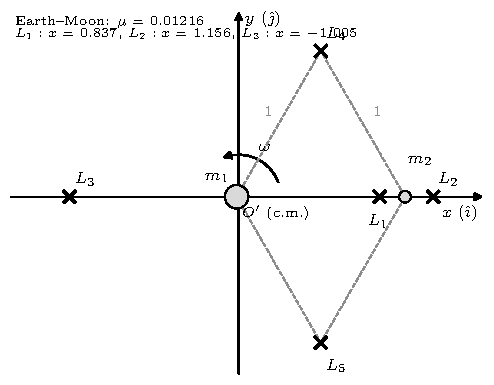
\includegraphics[width=0.5\linewidth]{lagrange}\end{center}

\paragraph{Equilibrium conditions.} Equilibrium requires zero velocity and zero acceleration in the synodic frame:
\begin{equation}
\dot x=\dot y=\dot z=0,\qquad \ddot x=\ddot y=\ddot z=0\;\Longrightarrow\;
\frac{\partial\Omega}{\partial x}=\frac{\partial\Omega}{\partial y}=\frac{\partial\Omega}{\partial z}=0,
\end{equation}
i.e.\ libration points are the stationary points of $\Omega$ (the Coriolis terms vanish because the velocity is zero).
$\Omega_z=-z\left[\frac{1-\mu}{r_1^3}+\frac{\mu}{r_2^3}\right]=0$ gives $z=0$: the points lie in the plane of the primaries. With
$r_1=\sqrt{(x+\mu)^2+y^2}$, $r_2=\sqrt{(x+\mu-1)^2+y^2}$:
\begin{equation}
\sys{\text{(A)}\quad&\Omega_x=x-\frac{(1-\mu)(x+\mu)}{r_1^{3}}-\frac{\mu(x+\mu-1)}{r_2^{3}}=0\\
\text{(B)}\quad&\Omega_y=y-\frac{(1-\mu)\,y}{r_1^{3}}-\frac{\mu\,y}{r_2^{3}}=0}
\end{equation}

\paragraph{Collinear points.} They are sought on the $x$-axis, $y=0$: (B) is then satisfied identically, and only (A) remains,
with $r_1=|x+\mu|$, $r_2=|x+\mu-1|$:
\begin{equation}
\boxed{\;x-\frac{(1-\mu)(x+\mu)}{|x+\mu|^{3}}-\frac{\mu\,(x+\mu-1)}{|x+\mu-1|^{3}}=0\;}
\end{equation}
Physically: gravity of the two primaries balances the centrifugal term $x$ (the point co-rotates with the primaries). The
absolute values split the axis into three intervals; in each one the equation becomes a quintic polynomial in $x$ with a single
admissible real root:
\begin{itemize}
\item[(a)] $x<-\mu$ (beyond $m_1$): $r_1=-(x+\mu)$, $r_2=1-\mu-x$ $\Rightarrow$ \textbf{$L_3$}, left exterior point;
\item[(b)] $-\mu<x<1-\mu$ (between the primaries): $r_1=x+\mu$, $r_2=1-\mu-x$ $\Rightarrow$ \textbf{$L_1$}, interior point;
\item[(c)] $x>1-\mu$ (beyond $m_2$): $r_1=x+\mu$, $r_2=x+\mu-1$ $\Rightarrow$ \textbf{$L_2$}, right exterior point.
\end{itemize}
For example, for $L_1$ with $\gamma=r_2$ (distance from $m_2$), $x=1-\mu-\gamma$, $r_1=1-\gamma$:
\begin{equation}
1-\mu-\gamma-\frac{1-\mu}{(1-\gamma)^2}+\frac{\mu}{\gamma^2}=0,
\end{equation}
which, multiplied by $\gamma^2(1-\gamma)^2$, is a quintic in $\gamma$ \notinnotes. For small $\mu$, $\gamma\approx(\mu/3)^{1/3}$ for both
$L_1$ and $L_2$ (Hill sphere) \notinnotes. Earth--Moon ($\mu=0.01216$): $x_{L_1}=0.8369$, $x_{L_2}=1.1557$, $x_{L_3}=-1.0051$ DU,
i.e.\ $L_1$ about 58\,000\,km and $L_2$ about 64\,500\,km from the Moon.

\paragraph{For completeness: triangular points.} If $y\neq0$, (B) divided by $y$ gives $1-\frac{1-\mu}{r_1^3}-\frac{\mu}{r_2^3}=0$, satisfied by
$r_1=r_2=1$; inserted in (A): $x-(1-\mu)(x+\mu)-\mu(x+\mu-1)=0$ identically. Hence $L_4$, $L_5$ at the vertices of the two
equilateral triangles built on the primaries.

\begin{keyf}
Equilibrium $\Leftrightarrow\nabla\Omega=\underline 0$ ($z=0$); collinear ($y=0$): $x-\dfrac{(1-\mu)(x+\mu)}{r_1^3}-\dfrac{\mu(x+\mu-1)}{r_2^3}=0$,
$r_1=|x+\mu|$, $r_2=|x+\mu-1|$; intervals $x<-\mu$ ($L_3$), $-\mu<x<1-\mu$ ($L_1$), $x>1-\mu$ ($L_2$).
\end{keyf}

\pitfalls
\begin{itemize}
\item The condition is on $\nabla\Omega$, not on the gravitational force alone: the centrifugal term $x$ is essential.
\item Keep the absolute values (or the signs of $x+\mu$ and $x+\mu-1$) in each interval.
\item Naming: $L_1$ between the primaries, $L_2$ beyond $m_2$, $L_3$ beyond $m_1$.
\end{itemize}

\further
Stability (commented section of the notes): $\Omega$ is a saddle at $L_{1,2,3}$, which are \emph{unstable}; $L_{4,5}$ are minima of
$\Omega$ and, according to the linear analysis, neutrally stable if $\mu<\frac12-\frac{\sqrt{69}}{18}\simeq0.0385$ (Earth--Moon
satisfies it).

\source{cap05.tex l.469--508 (collinear points), l.510--535 (triangular points), l.537--571 ($\Omega$ at $L_i$); numerical roots
from \texttt{figures/src/make\_figures.py}.}

% ---------------------------------------------------------------------
\question{B4}{Synodic frame and proof of the Jacobi integral}
% source: cap05.tex l.259-413
\begin{qbox}
In the CR3BP, define the synodic frame and its coordinates $(x,y,z)$. Starting from
$\ddot x-2\dot y=\frac{\partial\Omega}{\partial x}$, $\ddot y+2\dot x=\frac{\partial\Omega}{\partial y}$, $\ddot z=\frac{\partial\Omega}{\partial z}$,
$\Omega=\frac{x^2+y^2}{2}+\frac{1-\mu}{r_1}+\frac{\mu}{r_2}$, prove (and give) the Jacobi integral.
\qmeta{$\times$2 in the list (2025); Sep 2024 ("Jacobi integral"); Jan 2025 ("from the equations with the derivatives of $\Omega$ to the
Jacobi integral"); Mar 2025 ("Jacobi integral").}
\qnote{Sep 2024 Q3 mentions "the same question as January about $\Omega$": if $\Omega$ is the CR3BP potential it is this question;
if it is the RAAN, see \qref{C3}.}
\end{qbox}

\begin{outline}
\begin{enumerate}
\item CR3BP hypotheses; synodic frame (origin, axes, rotation), canonical units, $\mu$, positions of the primaries; coordinates $(x,y,z)$.
\item (Optional) origin of the equations: acceleration in the rotating frame (Coriolis $2\omega$, centrifugal $\omega^2$).
\item Multiply by $\dot x,\dot y,\dot z$ and add: Coriolis terms cancel.
\item $\Omega=\Omega(x,y,z)$ only $\Rightarrow$ RHS $=d\Omega/dt$; LHS $=\frac12 dv^2/dt$ $\Rightarrow$ $C=2\Omega-v^2$ constant.
\item Meaning: integral of motion, related to energy ($C\downarrow$ when $\mathcal E\uparrow$); zero-velocity surfaces.
\end{enumerate}
\end{outline}

\answer
\paragraph{Problem and synodic frame.} CR3BP: a spacecraft of negligible mass moves under the attraction of two primaries
$m_1>m_2$ that describe circular orbits about their centre of mass with constant distance $R$ and angular velocity
$\omega=\sqrt{G(m_1+m_2)/R^3}$. The \textbf{synodic frame} $\{\hat\imath,\hat\jmath,\hat k\}$ has
\begin{itemize}
\item origin $O'$ at the centre of mass of the primaries;
\item $\hat\imath$ along the line joining the primaries, pointing from $m_1$ to $m_2$; $\hat k$ parallel to the angular momentum of the
primaries (normal to their orbit plane); $\hat\jmath=\hat k\times\hat\imath$;
\item it \textbf{rotates} with angular velocity $\underline\omega=\omega\hat k$ with respect to the inertial frame, so the primaries are fixed.
\end{itemize}
Canonical units: DU $=R$, TU $=1/\omega$ (so $\omega=1$ and $G(m_1+m_2)=1$); $\mu=m_2/(m_1+m_2)$, $m_1$ at $x=-\mu$, $m_2$ at
$x=1-\mu$. The coordinates $(x,y,z)$ are the components of $\underline r=x\hat\imath+y\hat\jmath+z\hat k$ in this rotating frame, and
$r_1=\sqrt{(x+\mu)^2+y^2+z^2}$, $r_2=\sqrt{(x+\mu-1)^2+y^2+z^2}$ are the distances from the primaries.

\paragraph{Where the equations come from.} Differentiating $\underline r=x\hat\imath+y\hat\jmath+z\hat k$ twice with
$\dot{\hat\imath}=\omega\hat\jmath$, $\dot{\hat\jmath}=-\omega\hat\imath$:
$\ddot{\underline r}=(\ddot x-2\omega\dot y-\omega^2x)\hat\imath+(\ddot y+2\omega\dot x-\omega^2y)\hat\jmath+\ddot z\hat k$
(Coriolis and centrifugal terms). Equating to the gravitational acceleration of the two primaries and moving the centrifugal terms
to the right-hand side gives the given equations with the pseudo-potential $\Omega$ (centrifugal + gravitational).

\paragraph{Proof.} Multiply the three equations by $\dot x$, $\dot y$, $\dot z$ respectively and add:
\begin{equation}
\dot x\ddot x-2\dot x\dot y+\dot y\ddot y+2\dot y\dot x+\dot z\ddot z
=\dot x\frac{\partial\Omega}{\partial x}+\dot y\frac{\partial\Omega}{\partial y}+\dot z\frac{\partial\Omega}{\partial z}.
\end{equation}
\begin{itemize}
\item The Coriolis terms cancel: $-2\dot x\dot y+2\dot y\dot x=0$ (the Coriolis acceleration is orthogonal to the relative velocity
and does no work).
\item Left-hand side: $\dot x\ddot x+\dot y\ddot y+\dot z\ddot z=\frac12\frac{d}{dt}\left(\dot x^2+\dot y^2+\dot z^2\right)$.
\item Right-hand side: $\Omega$ depends only on $(x,y,z)$, \emph{not explicitly on time} (the primaries are fixed in the synodic frame),
so the chain rule gives $\Omega_x\dot x+\Omega_y\dot y+\Omega_z\dot z=\frac{d\Omega}{dt}$.
\end{itemize}
Therefore
\begin{equation}
\frac12\frac{d}{dt}\left(\dot{x}^{2}+\dot{y}^{2}+\dot{z}^{2}\right)=\frac{d\Omega}{dt}
\;\Longrightarrow\;
\frac{d}{dt}\left[\Omega-\tfrac12\left(\dot{x}^{2}+\dot{y}^{2}+\dot{z}^{2}\right)\right]=0,
\end{equation}
\begin{equation}
\boxed{\;C:=2\Omega(x,y,z)-\left(\dot{x}^{2}+\dot{y}^{2}+\dot{z}^{2}\right)=\text{const}\;}\qquad
2\Omega=x^2+y^2+\frac{2(1-\mu)}{r_1}+\frac{2\mu}{r_2}.
\end{equation}

\paragraph{Meaning.} $C$ (Jacobi constant) is the only known integral of motion of the CR3BP; it is fixed by the initial conditions,
$C=2\Omega(\underline r_0)-v_0^2$ with $v_0$ the velocity \emph{relative to the synodic frame}. It plays the role of an energy:
$C$ \textbf{decreases as the mechanical energy increases} (e.g.\ after a $\Delta v$ that increases the speed). It is not the
inertial energy, which is not conserved because the primaries move. Since $v^2=2\Omega-C\ge0$, it defines the
\textbf{zero-velocity surfaces} $2\Omega=C$, which bound the regions of possible motion (Hill's regions); see \qref{B1}.

\begin{keyf}
$\ddot x-2\dot y=\Omega_x$, $\ddot y+2\dot x=\Omega_y$, $\ddot z=\Omega_z$; \ $\times(\dot x,\dot y,\dot z)$ and sum $\Rightarrow$
$\frac12\frac{d}{dt}v^2=\frac{d\Omega}{dt}$; \ $C=2\Omega-(\dot x^2+\dot y^2+\dot z^2)$, $\Omega=\frac{x^2+y^2}{2}+\frac{1-\mu}{r_1}+\frac{\mu}{r_2}$.
\end{keyf}

\pitfalls
\begin{itemize}
\item The key step is that $\Omega$ is time-independent in the synodic frame; say it explicitly.
\item Show the cancellation of the Coriolis terms.
\item $v$ is the velocity relative to the rotating frame; $C$ is not the energy (it decreases when the energy increases).
\item With dimensional units the equations contain $\omega$ ($\ddot x-2\omega\dot y$, $\frac{\omega^2}{2}(x^2+y^2)$); the proof is identical.
\end{itemize}

\further
In terms of inertial quantities, $C=-2(\mathcal E-\omega H_z)$, where $\mathcal E$ and $H_z$ are the inertial specific energy and angular
momentum component of the spacecraft: neither is conserved separately, but this combination is \notinnotes.

\source{cap05.tex l.244--305 (CR3BP and synodic frame), l.307--378 (equations of motion), l.379--413 (Jacobi integral),
l.415--467 (zero-velocity surfaces). Formulario: not included (theory only).}

% ---------------------------------------------------------------------
\question{B5}{Synodic frame: origin, positions and gravitational parameters of the primaries}
% source: cap05.tex l.111-236 (two-body problem, omega), l.244-305 (synodic frame)
\begin{qbox}
In the CR3BP, define the synodic frame and locate its origin. Show analytically how to obtain the positions of the two primaries in
terms of the mass ratio $\mu$ and give their gravitational parameters in terms of $\mu$.
\qmeta{list by chapter (Ch.\,5).}
\end{qbox}

\begin{outline}
\begin{enumerate}
\item Hypotheses of the CR3BP; the primaries move on circles about their centre of mass $O'$ (two-body problem).
\item Synodic frame: origin $O'$, $\hat\imath$ towards $m_2$, $\hat k\parallel\underline H$, rotating with $\omega=\sqrt{GM/R^3}$; rotation matrix.
\item Positions: $x_2-x_1=R$ and $m_1x_1+m_2x_2=0$ $\Rightarrow$ $x_1=-\frac{m_2}{M}R$, $x_2=\frac{m_1}{M}R$.
\item Canonical units DU $=R$, TU $=1/\omega$ $\Rightarrow$ $GM=$ DU$^3$/TU$^2$; $\mu=m_2/M$: $x_1=-\mu$, $x_2=1-\mu$; $Gm_1=1-\mu$, $Gm_2=\mu$.
\end{enumerate}
\end{outline}

\answer
\paragraph{Motion of the primaries.} In the two-body problem the centre of mass $O'$ of $m_1$ and $m_2$ moves uniformly and can be
taken as origin of an inertial frame; then $m_1\underline R_1+m_2\underline R_2=\underline 0$ and each primary moves on a conic about
$O'$, the two conics having the same eccentricity, with $a_1/a_2=m_2/m_1$ and mean motion $\omega^2=G M/(a_1+a_2)^3$,
$M=m_1+m_2$. In the CR3BP the primaries move on \textbf{circles} ($e=0$) at constant distance $R=a_1+a_2$, hence
\begin{equation}
\omega=\sqrt{\frac{G(m_1+m_2)}{R^{3}}}=\text{const}.
\end{equation}

\paragraph{Synodic frame.} Origin at $O'$ (centre of mass of the primaries); $\hat\imath$ along the line of the primaries pointing towards
$m_2$; $\hat k$ parallel to the angular momentum $\underline H$ of the primaries; $\hat\jmath$ completes the right-handed triad. It
rotates with them: if it coincides with the inertial frame $\{\hat c_i\}$ at $t=0$, $[\hat\imath\ \hat\jmath\ \hat k]^T=R_3(\omega t)[\hat c_1\ \hat c_2\ \hat c_3]^T$.
In this frame the primaries are at rest on the $x$-axis.

\paragraph{Positions of the primaries.} With $x_1<0<x_2$ the abscissas of $m_1$ and $m_2$:
\begin{equation}
\sys{&x_2-x_1=R\\ &m_1x_1+m_2x_2=0\ \text{(origin at the centre of mass)}}
\;\Longrightarrow\;
\sys{&x_1=-\frac{m_2}{m_1+m_2}\,R\\ &x_2=\frac{m_1}{m_1+m_2}\,R}
\end{equation}
(from the second equation $x_2=-\frac{m_1}{m_2}x_1$; substituting in the first: $-x_1\frac{m_1+m_2}{m_2}=R$).

\paragraph{Mass parameter and canonical units.} Define
\begin{equation}
\mu:=\frac{m_2}{m_1+m_2}\in\left(0,\tfrac12\right)\quad(m_1>m_2),\qquad \text{DU}=R,\qquad \text{TU}=\omega^{-1}.
\end{equation}
Then $\omega=1$ TU$^{-1}$ and, from $\omega^2=G(m_1+m_2)/R^3$, $G(m_1+m_2)=\dfrac{\text{DU}^3}{\text{TU}^2}$. Therefore
\begin{equation}
\boxed{\;x_1=-\mu\ \text{DU},\quad x_2=(1-\mu)\ \text{DU};\qquad
Gm_1=(1-\mu)\,\frac{\text{DU}^3}{\text{TU}^2},\quad Gm_2=\mu\,\frac{\text{DU}^3}{\text{TU}^2}\;}
\end{equation}
and the distance between the primaries is $x_2-x_1=1$ DU. This is why the equations of motion contain $(1-\mu)$ and $\mu$ as
gravitational parameters and $(x+\mu)$, $(x+\mu-1)$ in the distances. Since $\mu<\frac12$ the origin is closer to $m_1$.
Earth--Moon: $\mu=1/82.27=0.01216$, so the barycentre is at $\mu R\approx4670$\,km from the Earth's centre, i.e.\ inside the Earth
\notinnotes.

\begin{center}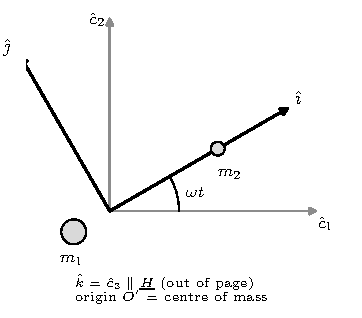
\includegraphics[width=0.36\linewidth]{synodic}\end{center}

\begin{keyf}
$\omega=\sqrt{G(m_1+m_2)/R^3}$; \ $x_1=-\dfrac{m_2}{M}R=-\mu$, \ $x_2=\dfrac{m_1}{M}R=1-\mu$; \ $\mu=\dfrac{m_2}{m_1+m_2}$; \
$Gm_1=1-\mu$, $Gm_2=\mu$ (DU$^3$/TU$^2$).
\end{keyf}

\pitfalls
\begin{itemize}
\item The origin is the centre of mass, \emph{not} the centre of $m_1$.
\item $\mu$ is the mass fraction of the \emph{smaller} primary; $m_1$ is at $-\mu$, $m_2$ at $1-\mu$.
\item Show the two equations (distance and centre of mass) and the step $G(m_1+m_2)=1$ in canonical units.
\end{itemize}

\source{cap05.tex l.111--236 (problem of two bodies, $\omega^2=GM/(a_1+a_2)^3$), l.244--305 (CR3BP, synodic frame, positions and
gravitational parameters).}

% ---------------------------------------------------------------------
\question{B6}{Integrals of motion of the $N$-body problem; the Laplace plane}
% source: cap05.tex l.28-109
\begin{qbox}
Identify the integrals of motion in the problem of $N$ bodies ($\underline R_i$ and $\dot{\underline R}_i$ are the position and velocity of
each point mass $m_i$ in a generic inertial frame) and provide their expressions. Prove that the angular momentum is constant.
Define the invariant Laplace plane and provide the expression of the remarkable vector orthogonal to this plane.
\qmeta{$\times$2 in the list (2025); Jun 2025; Sep 2025 (only: Laplace plane and the vector orthogonal to it).}
\qnote{If only the Laplace plane is asked (Sep 2025): write the equations of motion, the definition of $\underline H_c$, the proof
that it is constant and the definition of the plane (points 1, 4, 5 of the outline).}
\end{qbox}

\begin{outline}
\begin{enumerate}
\item Equations: $m_i\ddot{\underline R}_i=\sum_{j\neq i}Gm_im_j\underline r_{ij}/r_{ij}^3$; internal forces sum to zero.
\item Linear momentum $\sum m_i\dot{\underline R}_i=\underline a$ and centre of mass $\sum m_i\underline R_i=\underline at+\underline b$ (6 integrals).
\item Energy $\mathcal E=T+U$ constant (1 integral).
\item Angular momentum about $C$: $\underline H_c=\sum\underline r_i\times m_i\dot{\underline R}_i$; proof $\dot{\underline H}_c=\underline 0$ (3 integrals).
\item Laplace (invariant) plane: through $C$, orthogonal to $\underline H_c$. Total: 10 integrals.
\end{enumerate}
\end{outline}

\answer
\paragraph{Equations of motion.} $N$ point masses $m_i$, positions $\underline R_i$ in an inertial frame centred in $O$; only mutual
gravitational attraction:
\begin{equation}
m_{i}\,\ddot{\underline R}_{i}=G\sum_{j=1,\,j\neq i}^{N}\frac{m_{i}m_{j}}{r_{ij}^{3}}\,\underline{r}_{ij},\qquad
\underline r_{ij}=\underline R_j-\underline R_i,\ \ r_{ij}=|\underline r_{ij}|.
\end{equation}
The gravitational forces are \emph{internal} and act in equal and opposite pairs ($\underline r_{ji}=-\underline r_{ij}$), so their vector
sum is zero.

\paragraph{1. Linear momentum and centre of mass (6 scalar integrals).} Summing over $i$:
\begin{equation}
\sum_{i=1}^{N}m_i\ddot{\underline R}_i=\underline 0\;\Longrightarrow\;
\sum_{i=1}^{N}m_i\dot{\underline R}_i=\underline a,\qquad \sum_{i=1}^{N}m_i\underline R_i=\underline a\,t+\underline b,
\end{equation}
with $\underline a$, $\underline b$ constant vectors fixed by the initial conditions. The centre of mass
$\underline R_c=\frac{1}{M}\sum m_i\underline R_i$ ($M=\sum m_i$) moves in uniform rectilinear motion: $\underline R_c(t)=(\underline at+\underline b)/M$.

\paragraph{2. Energy (1 scalar integral).} Gravity is conservative, so the total energy (kinetic plus potential,
$U=-\sum_{i<j}Gm_im_j/r_{ij}$) is constant:
\begin{equation}
\mathcal E=\frac12\sum_{i=1}^{N}m_i\,\dot{\underline R}_i\cdot\dot{\underline R}_i-\sum_{i<j}G\frac{m_im_j}{r_{ij}}=\text{const}.
\end{equation}

\paragraph{3. Angular momentum about the centre of mass (3 scalar integrals).}
\begin{equation}
\underline H_c=\sum_{i=1}^{N}\underline r_i\times m_i\dot{\underline R}_i,\qquad \underline r_i=\underline R_i-\underline R_c .
\end{equation}
\emph{Proof that it is constant}:
\begin{equation}
\dot{\underline H}_c=\sum_i(\dot{\underline R}_i-\dot{\underline R}_c)\times m_i\dot{\underline R}_i+\sum_i(\underline R_i-\underline R_c)\times m_i\ddot{\underline R}_i .
\end{equation}
\begin{itemize}
\item First sum: $\sum_i\dot{\underline R}_i\times m_i\dot{\underline R}_i=\underline 0$; the rest is $-\dot{\underline R}_c\times\sum_im_i\dot{\underline R}_i=-\dot{\underline R}_c\times M\dot{\underline R}_c=\underline 0$.
\item Second sum: $-\underline R_c\times\sum_im_i\ddot{\underline R}_i=\underline 0$ by point 1; the remaining term is
\begin{equation}
\sum_i\underline R_i\times m_i\ddot{\underline R}_i=\sum_i\sum_{j\neq i}G\frac{m_im_j}{r_{ij}^3}\,\underline R_i\times(\underline R_j-\underline R_i)
=\sum_i\sum_{j\neq i}G\frac{m_im_j}{r_{ij}^3}\,\underline R_i\times\underline R_j=\underline 0,
\end{equation}
because the coefficient is symmetric in $(i,j)$ while $\underline R_i\times\underline R_j=-\underline R_j\times\underline R_i$: the terms cancel in pairs
(the mutual forces are central, along the line joining the two masses).
\end{itemize}
Hence $\dot{\underline H}_c=\underline 0$: $\underline H_c$ is conserved.

\paragraph{Laplace (invariant) plane.} It is the plane through the centre of mass $C$ \textbf{orthogonal to $\underline H_c$}. Its normal
\begin{equation}
\hat n=\frac{\underline H_c}{|\underline H_c|},\qquad
\underline H_c=\sum_{i=1}^{N}(\underline R_i-\underline R_c)\times m_i\dot{\underline R}_i
\end{equation}
is fixed in inertial space whatever the subsequent motion of the bodies: the plane is \emph{invariable}. It is the natural
reference plane of a planetary system (for the Solar System it is close to the orbit plane of Jupiter \notinnotes).
\begin{center}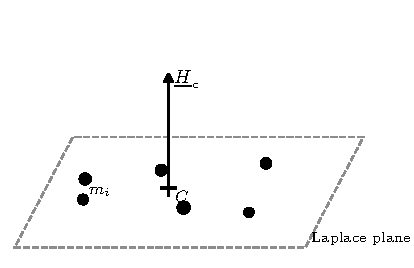
\includegraphics[width=0.42\linewidth]{nbody}\end{center}

\paragraph{Count.} $\underline a$ (3) $+$ $\underline b$ (3) $+$ $\mathcal E$ (1) $+$ $\underline H_c$ (3) $=$ \textbf{10 scalar integrals}, fixed
by the initial conditions and preserved regardless of the evolution of each individual mass. They are not enough to
integrate the problem for $N\ge3$ (the motion is in general chaotic).

\begin{keyf}
$\sum m_i\dot{\underline R}_i=\underline a$, \ $\sum m_i\underline R_i=\underline at+\underline b$, \ $\mathcal E=\frac12\sum m_i\dot R_i^2-\sum_{i<j}\frac{Gm_im_j}{r_{ij}}$,
\ $\underline H_c=\sum(\underline R_i-\underline R_c)\times m_i\dot{\underline R}_i$; Laplace plane $\perp\underline H_c$ through $C$; 10 integrals.
\end{keyf}

\pitfalls
\begin{itemize}
\item In the proof, show \emph{why} the double sum vanishes (symmetric coefficients, antisymmetric cross product).
\item The Laplace plane is orthogonal to $\underline H_c$ and passes through the centre of mass.
\item Do not confuse $\underline r_i=\underline R_i-\underline R_c$ (position w.r.t.\ $C$) with $\underline r_{ij}$ (mutual position).
\end{itemize}

\further
The angular momentum about the inertial origin, $\underline H_O=\underline H_c+M\underline R_c\times\dot{\underline R}_c$, is also constant, since
$\underline R_c\times\dot{\underline R}_c=(\underline b\times\underline a)/M^2$ \notinnotes. For $N=2$ these integrals reduce the problem to a
Keplerian relative motion (\qref{E10}).

\source{cap05.tex l.28--109 (problem of $N$ bodies: integrals, proof, Laplace plane).}

% =====================================================================
% Group C -- Chapter 8: orbit perturbations (one question per exam)
% Source: latex_notes/SFM_08_Orbit Perturbations/cap08.tex
% =====================================================================
\qgroup{C}{Chapter 8 -- Orbit perturbations}

One of the three orbital-mechanics questions is always on Chapter 8. Per the course program, for SRP and drag only the
definition, the expression and the overall effect may be asked (not the derivation of the exact components), and for the
third body the positions of Sun and Moon are not requested.

Perturbed motion: $\ddot{\underline r}=-\frac{\mu}{r^3}\underline r+\underline f$; $\underline h$ and $\underline e$ are no longer constant:
$\dot{\underline h}=\underline r\times\underline f$. Order of magnitude at 1000\,km of altitude ($a_0=\mu/r^2$):
$a_{J2}\simeq10^{-2}a_0$, $a_{3B}\simeq10^{-7}a_0$, $a_{RP}\simeq10^{-9}a_0$, $a_D\simeq10^{-10}a_0$.
Asphericity and third body are conservative; drag and SRP are \emph{surface} perturbations (depend on the spacecraft area);
all of them except SRP depend on the altitude.

\begin{center}
\small
\begin{tabular}{@{}lllr@{}}
\toprule
Q & Topic & Asked & Page\\
\midrule
\ref{q:C1} & Solar radiation pressure: nature and formula & $\times$3, Jan 2023 & \pageref{q:C1}\\
\ref{q:C2} & SRP + geometry of eclipses & Jun 2025 & \pageref{q:C2}\\
\ref{q:C3} & $J_2$: nature, two averaged effects, lat/long dependence & list & \pageref{q:C3}\\
\ref{q:C4} & $J_2$ and $J_{22}$: meridians and parallels & list, Sep 2024 & \pageref{q:C4}\\
\ref{q:C5} & Three types of harmonics; $J_{32}$ & list, Sep 2024 & \pageref{q:C5}\\
\ref{q:C6} & Sun-synchronous orbits & list & \pageref{q:C6}\\
\ref{q:C7} & Third body: exact acceleration, effect on $\underline h$ & list, Jan 2025 & \pageref{q:C7}\\
\ref{q:C8} & Gravity-gradient dyadic & $\times$2, Feb 2025, Sep 2025 & \pageref{q:C8}\\
\ref{q:C9} & Drag: acceleration and effect on $a$, $e$ & Jul 2025, Mar 2025 & \pageref{q:C9}\\
\bottomrule
\end{tabular}
\end{center}

% ---------------------------------------------------------------------
\question{C1}{Solar radiation pressure: physical nature and perturbing acceleration}
% source: cap08.tex l.41-60 (intro), l.561-687 (SRP), l.714-726 (effect)
\begin{qbox}
Describe the physical nature of solar-radiation pressure; write the fundamental formula for the perturbing acceleration,
identifying and explaining each term.
\qmeta{$\times$3 in the list (2025); Jan 2023.}
\qnote{\qref{C2} is the same question plus the geometry of the Earth's shadow.}
\end{qbox}

\begin{outline}
\begin{enumerate}
\item Nature: electromagnetic radiation carries momentum; absorbed/reflected photons exert a pressure on the surface.
\item Intensity: $S=S_0(R_0/R)^2$; at 1\,AU $S_E=1367$\,W/m$^2$; pressure $P_{SR}=S_E/c=4.56\cdot10^{-6}$\,N/m$^2$.
\item Formula $\underline f^{(SR)}=-\nu\,\frac{P_{SR}A}{m}\,C_R\,\hat r_{SUN}$ (cannon-ball model) and meaning of $\nu$, $A$, $m$, $C_R\in[1,2]$, $\hat r_{SUN}$.
\item Characteristics: surface, independent of altitude, important at high orbits; effect: all elements, $\underline e$ orthogonal to the Sun direction.
\end{enumerate}
\end{outline}

\answer
\paragraph{Physical nature.} Solar radiation is electromagnetic radiation, and photons carry linear momentum ($p=E/c$). When
radiation hits the spacecraft surface, the absorbed photons transfer their momentum and the reflected ones transfer about
twice as much: the result is a small force on the illuminated surface, i.e.\ a \emph{pressure}. It is a \textbf{surface} perturbation
(it depends on the area exposed and on the optical properties of the surface) and, unlike all other perturbations, it does
\textbf{not depend on the altitude} of the orbit, only on the distance from the Sun.

\paragraph{Radiation pressure.} The radiated power intensity at the photosphere is $S_0=63.15\cdot10^6$\,W/m$^2$; radiation follows the
inverse-square law, so at a distance $R$ from the Sun centre
\begin{equation}
S=S_{0}\left(\frac{R_{0}}{R}\right)^{2},\qquad R_0=696\,000\ \text{km (photospheric radius)}.
\end{equation}
At the Earth's distance ($1\,\text{AU}=149.6\cdot10^6$\,km) $S_E=1367$\,W/m$^2$ (\emph{solar constant}). Dividing by the speed of light:
\begin{equation}
P_{SR}=\frac{S_{E}}{c}=4.56\cdot10^{-6}\ \frac{\text{N}}{\text{m}^{2}}.
\end{equation}

\paragraph{Perturbing acceleration (cannon-ball model).} The spacecraft is modelled as a sphere of radius $\sigma$:
\begin{equation}
\boxed{\;\underline{f}^{(SR)}=-\nu\,\frac{P_{SR}\,A}{m}\,C_{R}\,\hat{r}_{\text{SUN}}\;}
\end{equation}
\begin{itemize}
\item $\nu$ = \textbf{shadow function}: $\nu=1$ if the spacecraft is illuminated, $\nu=0$ if it is in the Earth's shadow (eclipse).
\item $P_{SR}$ = solar radiation pressure at the spacecraft distance from the Sun (4.56\,$\mu$N/m$^2$ at 1\,AU).
\item $A=\pi\sigma^2$ = \textbf{illuminated cross-section} (area projected on the plane normal to the Sun rays).
\item $m$ = spacecraft mass; $A/m$ (area-to-mass ratio) measures the sensitivity to SRP: large, light structures (solar sails,
balloons, large panels) are strongly affected.
\item $C_R$ = \textbf{radiation-pressure coefficient}, between 1 (totally absorbing surface) and 2 (totally reflecting surface). The
limits follow from conservation of linear momentum: a reflected photon reverses its momentum, so it transfers twice the
momentum of an absorbed one.
\item $\hat r_{SUN}$ = unit vector \textbf{from the spacecraft to the Sun}; the minus sign means the acceleration points away
from the Sun. Since $r\ll1$\,AU it can be approximated with the Earth-to-Sun direction:
$\underline r_{SUN}=1\,\text{AU}\,[c_{\theta_s}\ \ c_\epsilon s_{\theta_s}\ \ s_\epsilon s_{\theta_s}]\,[\hat c_1\ \hat c_2\ \hat c_3]^T$
($\epsilon$ = obliquity of the ecliptic, $\theta_s$ = ecliptic longitude of the Sun, increasing by $2\pi$ per sidereal year).
\end{itemize}
\begin{center}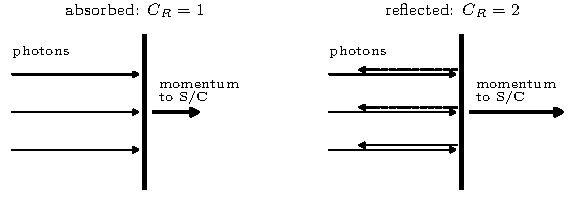
\includegraphics[width=0.62\linewidth]{srp}\end{center}

\paragraph{Effect on the orbit.} Projected on $(\hat r,\hat\theta,\hat h)$ the acceleration enters the Gauss equations. SRP perturbs
\textbf{all orbit elements}. Its relative importance grows with altitude (at 1000\,km $a_{RP}\sim10^{-9}a_0$; at GEO it is one of the main
perturbations together with the third body). For an initially circular orbit SRP adds velocity on one side of the orbit
(positive tangential acceleration, $P_1$) and removes it on the opposite side ($P_2$): the orbit becomes elliptic with an
\textbf{eccentricity vector orthogonal to $\hat r_{SUN}$}, which then precesses following the yearly motion of the Earth around the Sun.

\begin{keyf}
$S=S_0(R_0/R)^2$, \ $S_E=1367$\,W/m$^2$, \ $P_{SR}=S_E/c=4.56\cdot10^{-6}$\,N/m$^2$, \
$\underline f^{(SR)}=-\nu\dfrac{P_{SR}A}{m}C_R\hat r_{SUN}$, \ $1\le C_R\le2$, \ $A=\pi\sigma^2$.
\end{keyf}

\pitfalls
\begin{itemize}
\item $\hat r_{SUN}$ points from the spacecraft to the Sun: hence the minus sign (the push is away from the Sun).
\item $C_R=1$ absorbing, $C_R=2$ reflecting (not the reverse); justify with momentum conservation.
\item Do not forget the shadow function $\nu$: no SRP in eclipse.
\end{itemize}

\source{cap08.tex l.41--60 (classification), l.561--687 (SRP and Sun position), l.714--726 (effect on the elements). Formulario: not included (T only).}

% ---------------------------------------------------------------------
\question{C2}{Solar radiation pressure and the geometry of eclipses}
% source: cap08.tex l.561-726
\begin{qbox}
Outline the physical nature of solar radiation perturbation, provide the expression of the perturbing acceleration, and describe
the geometry of eclipsing due to Earth.
\qmeta{Jun 2025.}
\qnote{Difference from \qref{C1}: adds the shadow (eclipse) computation, i.e.\ how $\nu$ is evaluated.}
\end{qbox}

\begin{outline}
\begin{enumerate}
\item Nature (photon momentum, surface perturbation, independent of altitude); $S$, $S_E$, $P_{SR}=S_E/c$.
\item $\underline f^{(SR)}=-\nu\frac{P_{SR}A}{m}C_R\hat r_{SUN}$ and meaning of the terms.
\item Eclipse geometry: angle $\Theta$ between $\underline r$ and $\underline r_{SUN}$; $\theta_1=\arccos(R_E/r)$, $\theta_2=\arccos(R_E/r_{SUN})$; sketch.
\item Test: $\Theta>\theta_1+\theta_2$ shadow ($\nu=0$), otherwise illuminated ($\nu=1$); comments.
\end{enumerate}
\end{outline}

\answer
\paragraph{Physical nature and acceleration.} Photons carry momentum; when absorbed or reflected by the spacecraft surface they
exert a pressure. At distance $R$ from the Sun $S=S_0(R_0/R)^2$; at 1\,AU $S_E=1367$\,W/m$^2$ and the pressure is
$P_{SR}=S_E/c=4.56\cdot10^{-6}$\,N/m$^2$. With the cannon-ball model (sphere of radius $\sigma$):
\begin{equation}
\underline{f}^{(SR)}=-\nu\,\frac{P_{SR}\,A}{m}\,C_{R}\,\hat{r}_{\text{SUN}},
\end{equation}
$\nu$ shadow function (1 illuminated, 0 in shadow), $A=\pi\sigma^2$ illuminated area, $m$ mass, $C_R\in[1,2]$ radiation-pressure
coefficient (1 absorbing, 2 reflecting: a reflected photon transfers twice the momentum), $\hat r_{SUN}$ unit vector from the
spacecraft to the Sun ($\simeq$ Earth--Sun direction since $r\ll1$\,AU). It is a surface perturbation, independent of the
altitude, relevant for high orbits and for high $A/m$; it perturbs all elements and, on a circular orbit, creates an
eccentricity vector orthogonal to the Sun direction (see \qref{C1}).

\paragraph{Geometry of the eclipse (shadow computation).} The spacecraft is in shadow when the Earth (sphere of radius $R_E$) blocks
the line of sight between spacecraft and Sun. Let
\begin{equation}
\Theta=\arccos\!\left(\frac{\underline r\cdot\underline r_{SUN}}{|\underline r|\,|\underline r_{SUN}|}\right)
\end{equation}
be the angle, at the Earth's centre, between the spacecraft position $\underline r$ and the Sun position $\underline r_{SUN}$. Draw from the
spacecraft and from the Sun the lines tangent to the Earth: the radius to each tangent point is orthogonal to the tangent, so
\begin{equation}
\theta_{1}=\arccos\!\left(\frac{R_{E}}{|\underline r|}\right),\qquad
\theta_{2}=\arccos\!\left(\frac{R_{E}}{|\underline r_{SUN}|}\right)
\end{equation}
are the angles between $\underline r$ (resp.\ $\underline r_{SUN}$) and the radius to its tangent point. The segment spacecraft--Sun is tangent to the
Earth when $\Theta=\theta_1+\theta_2$. Hence
\begin{equation}
\boxed{\;\Theta>\theta_1+\theta_2\ \Rightarrow\ \text{SHADOW }(\nu=0),\qquad \Theta\le\theta_1+\theta_2\ \Rightarrow\ \text{ILLUMINATION }(\nu=1).\;}
\end{equation}
\begin{center}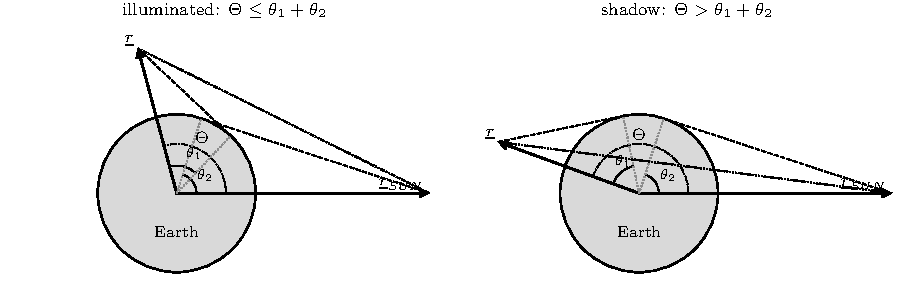
\includegraphics[width=0.9\linewidth]{eclipse}\\
{\footnotesize Not to scale ($r_{SUN}$ drawn small): in reality $\theta_2\simeq90^\circ$.}\end{center}

\paragraph{Comments.}
\begin{itemize}
\item Since $|\underline r_{SUN}|\gg R_E$, $\theta_2\simeq\pi/2$: the shadow is practically a cylinder of radius $R_E$ behind the Earth, and the
test becomes $\Theta>\pi/2+\theta_1$ \notinnotes.
\item The model is a sharp on/off shadow (no penumbra, spherical Earth, no atmospheric refraction) \notinnotes.
\item Eclipses make $\underline f^{(SR)}$ discontinuous along the orbit. Their duration is maximum when the Sun lies in the orbit plane:
for a circular orbit the shadow arc is $\pi-2\theta_1$, e.g.\ $r=7000$\,km: $\theta_1=24.3^\circ$, about 36\% of the period
(35\,min) \notinnotes. High orbits (GEO) are eclipsed only near the equinoxes.
\item Eclipses also matter for power (batteries) and thermal design.
\end{itemize}

\begin{fig2draw}
Earth circle with centre $O$; arrow $\underline r_{SUN}$ to the right, arrow $\underline r$ up-left; dashed tangent lines from the tip of each
arrow to the circle; mark $\theta_1$, $\theta_2$ at $O$ between each arrow and its tangent-point radius, and $\Theta$ between the arrows.
\end{fig2draw}

\begin{keyf}
$\underline f^{(SR)}=-\nu\dfrac{P_{SR}A}{m}C_R\hat r_{SUN}$; \ $\Theta=\arccos\dfrac{\underline r\cdot\underline r_{SUN}}{r\,r_{SUN}}$, \
$\theta_1=\arccos\dfrac{R_E}{r}$, \ $\theta_2=\arccos\dfrac{R_E}{r_{SUN}}$; \ shadow iff $\Theta>\theta_1+\theta_2$.
\end{keyf}

\pitfalls
\begin{itemize}
\item The angles $\theta_1$, $\theta_2$ are measured at the Earth's centre, between the position vectors and the radii to the tangent points.
\item Shadow for \emph{large} $\Theta$ (spacecraft behind the Earth), not small.
\end{itemize}

\source{cap08.tex l.561--687 (SRP), l.689--712 (shadow computation), l.714--726 (effect on the elements).}

% ---------------------------------------------------------------------
\question{C3}{$J_2$ perturbation: physical nature and averaged effects}
% source: cap08.tex l.728-836 (harmonics), l.838-949 (J2), l.951-1062 (averaging)
\begin{qbox}
Describe the physical nature of the $J_2$ perturbation, its two main averaged effects on orbital elements, and state whether it
depends on geographic latitude and/or longitude.
\qmeta{list by chapter (Ch.\,8).}
\qnote{Possibly the "question about $\Omega$" of Sep 2024 (regression of the node). Adjacent: \qref{C4}, \qref{C5}, \qref{C6}.}
\end{qbox}

\begin{outline}
\begin{enumerate}
\item Geopotential expansion; $J_2$ is the zonal harmonic of degree 2: Earth \textbf{oblateness} (equatorial bulge); dominant ($J_2=1.083\cdot10^{-3}$).
\item $U_{J2}=-\frac{\mu}{r}\left(\frac{R_E}{r}\right)^2J_2\frac{3s_\phi^2-1}{2}$: depends on latitude (and $r$), \textbf{not on longitude}; sign map ($\pm35.3^\circ$).
\item Perturbing acceleration (radial + northward) and averaging over one orbit: $\langle\dot a\rangle=\langle\dot e\rangle=\langle\dot i\rangle=0$.
\item Effect 1: precession of the orbit plane, $\langle\dot\Omega\rangle\propto-c_i$ (westward for direct orbits). Effect 2: rotation of the apsidal line, $\langle\dot\omega\rangle$; critical inclination $63.4^\circ$.
\item Applications: sun-synchronous orbits, frozen apsidal line (Molniya).
\end{enumerate}
\end{outline}

\answer
\paragraph{Physical nature.} The Earth is not a sphere with spherical mass distribution: its potential is expanded in harmonics
(Legendre polynomials $P_{lm}$),
\begin{equation}
U=\frac{\mu_E}{r}-\frac{\mu_E}{r}\sum_{l=2}^{\infty}\left(\frac{R_E}{r}\right)^{l}J_lP_{l0}(s_\phi)
+\frac{\mu_E}{r}\sum_{l=2}^{\infty}\sum_{m=1}^{l}\left(\frac{R_E}{r}\right)^{l}J_{lm}P_{lm}(s_\phi)\cos\!\left[m(\lambda_g-\lambda_{lm})\right].
\end{equation}
The first term is the Keplerian potential; $J_2$ (zonal harmonic of degree 2, $P_{20}=\frac{3s_\phi^2-1}{2}$) represents the
\textbf{oblateness} of the Earth, i.e.\ the equatorial bulge due to its rotation:
\begin{equation}
U_{J2}=-\frac{\mu_{E}}{r}\left(\frac{R_{E}}{r}\right)^{2}J_{2}\,\frac{3s_{\phi}^{2}-1}{2},\qquad J_2=1.083\cdot10^{-3}.
\end{equation}
$U_{J2}>0$ for $|\phi|<\arcsin(1/\sqrt3)=35.3^\circ$ (extra mass around the equator) and $U_{J2}<0$ for higher latitudes (less mass at
the poles). $J_2$ is about three orders of magnitude larger than any other harmonic, so it is the dominant perturbation in LEO and
MEO (at 1000\,km, $a_{J2}\simeq10^{-2}a_0$), decreasing rapidly with altitude ($\propto1/r^4$).

\paragraph{Dependence on latitude and longitude.} $U_{J2}$ depends only on $r$ and on the \textbf{latitude} $\phi$; it does \textbf{not depend on the
longitude} ($\partial U_{J2}/\partial\lambda_g=0$): the field is axially symmetric about the polar axis (zonal harmonic). Hence
the perturbing acceleration has only radial and northward components:
\begin{equation}
\underline f_{J2}=\frac{3\mu_E}{r^4}R_E^2J_2\left[\frac{3s_\phi^2-1}{2}\,\hat r-s_\phi c_\phi\,\hat N_L\right]
=\frac{3\mu_{E}}{r^{4}}R_{E}^{2}J_{2}\left[\frac{3s_{\theta_t}^{2}s_{i}^{2}-1}{2}\ \ \ -s_{i}^{2}s_{\theta_t}c_{\theta_t}\ \ \ -s_{i}c_{i}s_{\theta_t}\right]^{\!T}
\end{equation}
(components along $\hat r,\hat\theta,\hat h$). Through the orbit the satellite sweeps latitudes $|\phi|\le i$, so the effect depends on
the inclination.

\paragraph{Averaging.} The osculating elements show short-period oscillations, long-period oscillations and secular drifts. Averaging
the Gauss equations over one orbital period (changing variable from $t$ to $\theta_*$, $d/d\theta_*\simeq(r^2/h)\,d/dt$) removes the
short-period terms. Example for $\Omega$: $\langle\Omega'\rangle=\frac{1}{2\pi}\int_0^{2\pi}\frac{r^2}{h}\frac{rf_h s_{\theta_t}}{hs_i}d\theta_*=-\frac{3R_E^2J_2c_i}{2p^2}$, then
multiplied by the mean motion. The results are
\begin{equation}
\langle\dot a\rangle=\langle\dot e\rangle=\langle\dot i\rangle=0,\qquad
\langle\dot{\Omega}\rangle=-\frac{3R_{E}^{2}J_{2}\sqrt{\mu_{E}}}{2a^{7/2}(1-e^{2})^{2}}\,c_{i},\qquad
\langle\dot{\omega}\rangle=-\frac{3R_{E}^{2}J_{2}\sqrt{\mu_{E}}}{2a^{7/2}(1-e^{2})^{2}}\left(\frac52s_{i}^{2}-2\right).
\end{equation}
Size and shape of the orbit and its inclination are unchanged on average (conservative, axisymmetric field).

\paragraph{The two main effects.}
\begin{enumerate}
\item \textbf{Precession of the orbital plane (regression of the nodes).} $\langle\dot\Omega\rangle\neq0$ with $i$ constant: the angular momentum
vector rotates about $\hat c_3$ (the Earth's axis) with period $T_{prec}=2\pi/|\langle\dot\Omega\rangle|$. The precession is clockwise (westward,
$\langle\dot\Omega\rangle<0$) for direct orbits ($i<\pi/2$), counter-clockwise for retrograde ones, and zero for polar orbits. Physically, the
equatorial bulge exerts a torque that tries to pull the orbit plane towards the equator; like a gyroscope, the plane precesses
instead of changing $i$ \notinnotes. Faster for low, near-equatorial orbits (several degrees per day in LEO).
\item \textbf{Rotation of the apsidal line.} $\langle\dot\omega\rangle\neq0$: the periapsis direction rotates within the orbit plane (forward for
$i<63.4^\circ$, backward between $63.4^\circ$ and $116.6^\circ$). It vanishes at the \textbf{critical inclinations}
\begin{equation}
5s_i^2-4=0\ \Rightarrow\ i=\arcsin\frac{2}{\sqrt5}\simeq63.4^\circ\ \text{or}\ 116.6^\circ,
\end{equation}
where the apsidal line is "frozen" in space (used by highly elliptic Molniya orbits to keep the apogee over high latitudes \notinnotes).
\end{enumerate}
\begin{center}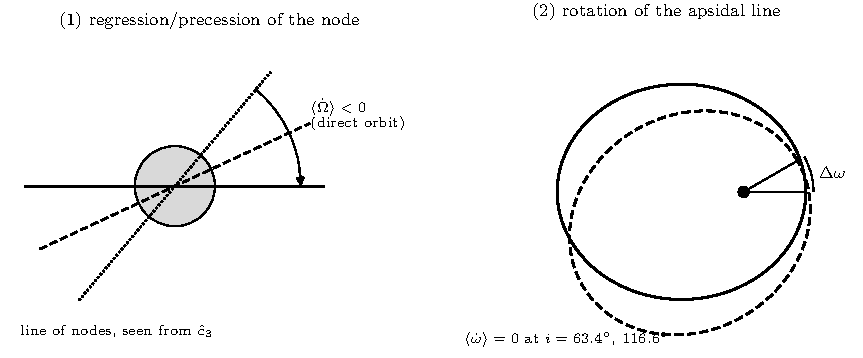
\includegraphics[width=0.85\linewidth]{j2_effects}\end{center}
Application: the nodal precession can be tuned to $360^\circ$/year to obtain \textbf{sun-synchronous orbits} (\qref{C6}).

\begin{keyf}
$U_{J2}=-\dfrac{\mu_E}{r}\left(\dfrac{R_E}{r}\right)^2J_2\dfrac{3s_\phi^2-1}{2}$; \ $\langle\dot a\rangle=\langle\dot e\rangle=\langle\dot i\rangle=0$; \
$\langle\dot\Omega\rangle=-\dfrac{3R_E^2J_2\sqrt{\mu_E}}{2a^{7/2}(1-e^2)^2}c_i$; \
$\langle\dot\omega\rangle=-\dfrac{3R_E^2J_2\sqrt{\mu_E}}{2a^{7/2}(1-e^2)^2}\left(\frac52s_i^2-2\right)$; \ $i_{crit}=63.4^\circ,\,116.6^\circ$.
\end{keyf}

\pitfalls
\begin{itemize}
\item $J_2$ depends on latitude only (zonal), not on longitude: say it explicitly with $\partial U_{J2}/\partial\lambda_g=0$.
\item Sign of $\langle\dot\Omega\rangle$: negative (westward) for direct orbits.
\item The secular effects are on $\Omega$ and $\omega$ (and on the mean motion), not on $a$, $e$, $i$.
\end{itemize}

\source{cap08.tex l.728--836 (geopotential harmonics), l.838--868 ($J_2$), l.870--949 (perturbing acceleration; errata \#12--13),
l.951--1062 (averaging, precession, critical inclinations). Formulario: \fml{8-J2V}, \fml{8-J2A}, \fml{8-PRC}.}

% ---------------------------------------------------------------------
\question{C4}{Physical nature of $J_2$ and $J_{22}$; meridians and parallels}
% source: cap08.tex l.728-868
\begin{qbox}
State the physical nature of $J_2$ and $J_{22}$ and how many meridians/parallels each corresponds to.
\qmeta{list by chapter (Ch.\,8); Sep 2024 (together with \qref{C5}).}
\end{qbox}

\begin{outline}
\begin{enumerate}
\item Geopotential expansion; $J_{lm}$ terms; rule: $J_{lm}$ has $l-m$ parallels and $m$ meridians as nodal (equipotential) lines.
\item $J_2=J_{20}$: zonal, Earth oblateness (equatorial bulge); $P_{20}=0$ at $\phi=\pm35.3^\circ$: 2 parallels, 0 meridians; depends on latitude only.
\item $J_{22}$: sectoral, ellipticity of the equator; zero at $\lambda_g=30.1^\circ,120.1^\circ,210.1^\circ,300.1^\circ$: 2 meridians, 0 parallels; depends on longitude.
\item Magnitudes and effects ($J_2$ dominant in LEO/MEO; $J_{22}$ dominant at GEO by resonance). Sketch.
\end{enumerate}
\end{outline}

\answer
\paragraph{Geopotential.} The Earth's gravitational potential is written as a series of harmonics:
\begin{equation}
U=\frac{\mu_E}{r}-\frac{\mu_E}{r}\sum_{l\ge2}\left(\frac{R_E}{r}\right)^{l}J_lP_{l0}(s_\phi)
+\frac{\mu_E}{r}\sum_{l\ge2}\sum_{m=1}^{l}\left(\frac{R_E}{r}\right)^{l}J_{lm}P_{lm}(s_\phi)\cos\!\left[m(\lambda_g-\lambda_{lm})\right],
\end{equation}
\begin{equation}
P_{lm}(x)=\frac{1}{2^{l}l!}\left(1-x^{2}\right)^{m/2}\frac{d^{\,l+m}}{dx^{\,l+m}}\left[(x^{2}-1)^{l}\right],\qquad x=s_\phi .
\end{equation}
Each harmonic is a correction to the potential of a spherical Earth; its nodal lines (where the term vanishes) are parallels and/or
meridians. General rule: \textbf{$J_{lm}$ has $l-m$ parallels and $m$ meridians} as equipotential (zero) lines.

\paragraph{$J_2$ ($l=2$, $m=0$): zonal harmonic -- Earth oblateness.} Since $P_{20}=\frac{3s_\phi^2-1}{2}$,
\[U_{J2}=-\frac{\mu_E}{r}\left(\frac{R_E}{r}\right)^2J_2\,\frac{3s_\phi^2-1}{2}\]
depends only on latitude. It vanishes where
$s_\phi=\pm1/\sqrt3$, i.e.\ at $\phi=\pm35.3^\circ$: \textbf{2 parallels and 0 meridians} ($l-m=2$, $m=0$). It is positive in the
equatorial band and negative at high latitudes: it models the \textbf{equatorial bulge} (extra mass at the equator, less at the poles)
produced by the Earth's rotation. $J_2=1.083\cdot10^{-3}$, about $10^3$ times larger than any other coefficient: it dominates the
perturbations of LEO and MEO satellites (nodal regression, apsidal rotation, \qref{C3}).

\paragraph{$J_{22}$ ($l=m=2$): sectoral harmonic -- ellipticity of the equator.} $P_{22}=3(1-s_\phi^2)=3c_\phi^2$ never vanishes except at the
poles, so the sign of the term is set by $\cos[2(\lambda_g-\lambda_{22})]$: it depends on longitude and vanishes at
\begin{equation}
\lambda_g=30.1^\circ,\ 120.1^\circ,\ 210.1^\circ,\ 300.1^\circ\quad(90^\circ\text{ apart}),
\end{equation}
i.e.\ on \textbf{2 meridians (full great circles) and 0 parallels} ($l-m=0$, $m=2$), dividing the Earth into 4 sectors of alternating sign
("orange slices"). It is related to the modest \textbf{eccentricity (ellipticity) of the Earth's equator}: the equatorial section is slightly
elliptic, not circular. $J_{22}=1.816\cdot10^{-6}$ ($\lambda_{22}=-0.261$\,rad). Small, but it \textbf{dominates for geostationary orbits}: a GEO
satellite is fixed with respect to the Earth, so the longitude-dependent force always acts in the same direction (resonance) and
makes the satellite drift in longitude (station keeping needed).
\begin{center}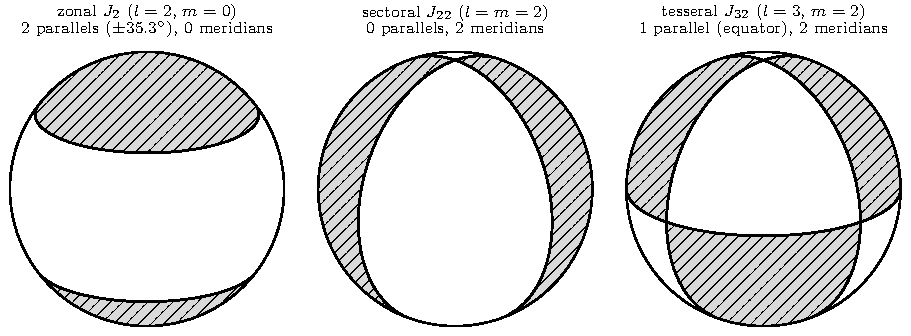
\includegraphics[width=0.9\linewidth]{harmonics}\\
{\footnotesize Sign maps of the three types of harmonics (hatched = negative), computed from $P_{lm}(s_\phi)\cos m\lambda$.}\end{center}

\begin{center}
\small
\begin{tabular}{@{}llllll@{}}
\toprule
 & type & physical meaning & depends on & parallels & meridians\\
\midrule
$J_2$ & zonal ($m=0$) & oblateness (equatorial bulge) & latitude & 2 ($\pm35.3^\circ$) & 0\\
$J_{22}$ & sectoral ($l=m$) & elliptic equator & longitude & 0 & 2 (4 sectors)\\
\bottomrule
\end{tabular}
\end{center}

\begin{keyf}
$J_{lm}$: $l-m$ parallels, $m$ meridians; \ $P_{20}=\frac{3s_\phi^2-1}{2}=0\Rightarrow\phi=\pm35.3^\circ$; \ $J_{22}$ zero at $\lambda_g=30.1^\circ+k\,90^\circ$; \
$J_2=1.083\cdot10^{-3}$, $J_{22}=1.816\cdot10^{-6}$.
\end{keyf}

\pitfalls
\begin{itemize}
\item "2 meridians" for $J_{22}$ means 2 great circles through the poles, i.e.\ 4 longitudes where the term vanishes.
\item $J_2$ = oblateness (polar flattening), $J_{22}$ = ellipticity of the \emph{equator}: different physical features.
\end{itemize}

\source{cap08.tex l.62--85 (perturbations on different orbits, $J_{22}$ at GEO), l.728--836 (harmonics, nodal lines, coefficients), l.838--868 ($J_2$).}

% ---------------------------------------------------------------------
\question{C5}{The three types of geopotential harmonics; the $J_{32}$ harmonic}
% source: cap08.tex l.728-836
\begin{qbox}
Describe the three types of geopotential harmonics; indicate whether they depend on latitude, longitude, or both, and give the
number and type of equipotential lines for the $J_{32}$ harmonic.
\qmeta{list by chapter (Ch.\,8); Sep 2024 (together with \qref{C4}: "also discuss the physical nature of $J_2$ and $J_{22}$").}
\qnote{In Sep 2024 this question was asked together with C4: write C5 and then the two paragraphs on $J_2$ and $J_{22}$ of C4.}
\end{qbox}

\begin{outline}
\begin{enumerate}
\item Geopotential series with $J_l$ and $J_{lm}$, $P_{lm}(s_\phi)$, $\cos m(\lambda_g-\lambda_{lm})$; first term = spherical Earth.
\item Zonal ($m=0$): latitude only, $l$ parallels (bands); e.g.\ $J_2$.
\item Sectoral ($l=m$): longitude only (sign), $m$ meridians (sectors); e.g.\ $J_{22}$.
\item Tesseral ($0<m<l$): latitude and longitude, $l-m$ parallels and $m$ meridians (tiles).
\item $J_{32}$: tesseral, 1 parallel (equator) + 2 meridians, 8 tiles; sketch.
\end{enumerate}
\end{outline}

\answer
\paragraph{Expansion of the geopotential.} The potential of the Earth, $U=G\int_{Earth}dm/r$, is written in terms of Legendre polynomials
(latitude $\phi$, geographical longitude $\lambda_g$):
\begin{equation}
U=\underbrace{\frac{\mu_E}{r}}_{U_K}
-\frac{\mu_E}{r}\sum_{l=2}^{\infty}\left(\frac{R_E}{r}\right)^{l}J_lP_{l0}(s_\phi)
+\frac{\mu_E}{r}\sum_{l=2}^{\infty}\sum_{m=1}^{l}\left(\frac{R_E}{r}\right)^{l}J_{lm}P_{lm}(s_\phi)\cos\!\left[m(\lambda_g-\lambda_{lm})\right].
\end{equation}
$U_K=\mu_E/r$ is the potential of a body with spherical symmetry (Keplerian motion); the other terms are the harmonics, with
coefficients $J_l$, $J_{lm}$, $\lambda_{lm}$ estimated from satellite tracking (WGS-84, EGM-96, JGM-2, EGM2008). The perturbing
acceleration is $\underline g=\nabla U$.

\paragraph{The three types.}
\begin{enumerate}[label=(\alph*)]
\item \textbf{Zonal harmonics} ($m=0$, coefficients $J_l$): $P_{l0}(s_\phi)$ \textbf{depends only on latitude}. They vanish at $l$ values of latitude:
the nodal lines are \textbf{$l$ parallels} and the Earth is divided in latitude bands (zones). Example: $J_2$ vanishes at $\pm35.3^\circ$
(oblateness).
\item \textbf{Sectoral harmonics} ($l=m$, coefficients $J_{ll}$): $P_{ll}\propto c_\phi^{\,l}$ does not vanish except at the poles, so the sign of the
term changes only with longitude: they \textbf{depend (in sign) only on longitude}. Nodal lines: \textbf{$m$ meridians}, which split the Earth
into $2m$ sectors. Example: $J_{22}$, zero at $\lambda_g=30.1^\circ,120.1^\circ,210.1^\circ,300.1^\circ$ (ellipticity of the equator).
\item \textbf{Tesseral harmonics} ($0<m<l$, coefficients $J_{lm}$): \textbf{depend on both latitude and longitude}; they vanish at given latitudes
\emph{and} longitudes, so the nodal lines (\textbf{$l-m$ parallels and $m$ meridians}) divide the Earth into tiles ("tesserae").
\end{enumerate}
General rule: \textbf{$J_{lm}$ has $l-m$ parallels and $m$ meridians as equipotential lines} (zonal: $m=0$; sectoral: $l-m=0$).

\paragraph{The $J_{32}$ harmonic.} $l=3$, $m=2$: \textbf{tesseral}. From the definition,
$P_{32}(x)=\frac{1}{48}(1-x^2)\frac{d^5}{dx^5}(x^2-1)^3=15x(1-x^2)$, so the term is proportional to
\begin{equation}
15\,s_\phi c_\phi^2\cos\!\left[2(\lambda_g-\lambda_{32})\right],
\end{equation}
which vanishes on
\begin{itemize}
\item $l-m=1$ \textbf{parallel}: the \textbf{equator} ($s_\phi=0$);
\item $m=2$ \textbf{meridians}: $\lambda_g=\lambda_{32}\pm45^\circ$ and $\lambda_{32}\pm135^\circ$ (two great circles through the poles).
\end{itemize}
The equipotential lines divide the Earth into $2\times4=8$ tiles of alternating sign. $J_{32}=3.774\cdot10^{-6}$,
$\lambda_{32}=-0.300$\,rad.
\begin{center}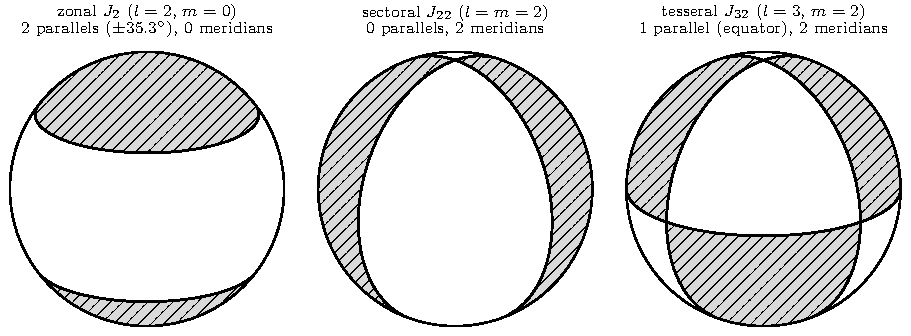
\includegraphics[width=0.9\linewidth]{harmonics}\end{center}

\begin{center}
\small
\begin{tabular}{@{}lllll@{}}
\toprule
type & indices & depends on & nodal lines & example\\
\midrule
zonal & $m=0$ & latitude & $l$ parallels & $J_2$: $\pm35.3^\circ$\\
sectoral & $m=l$ & longitude & $m$ meridians & $J_{22}$: 2 meridians\\
tesseral & $0<m<l$ & both & $l-m$ parallels, $m$ meridians & $J_{32}$: equator + 2 meridians\\
\bottomrule
\end{tabular}
\end{center}

\begin{fig2draw}
Three circles (globes). Zonal: two horizontal lines (parallels) symmetric about the equator, polar caps hatched. Sectoral: two
"meridian" curves through the poles, alternate sectors hatched. Tesseral $J_{32}$: the equator plus two meridians, checkerboard hatching.
\end{fig2draw}

\begin{keyf}
$U=\dfrac{\mu_E}{r}-\dfrac{\mu_E}{r}\displaystyle\sum_l\left(\frac{R_E}{r}\right)^lJ_lP_{l0}+\dfrac{\mu_E}{r}\sum_{l,m}\left(\frac{R_E}{r}\right)^lJ_{lm}P_{lm}\cos m(\lambda_g-\lambda_{lm})$; \
$J_{lm}$: $l-m$ parallels, $m$ meridians; \ $J_{32}$: 1 parallel (equator) + 2 meridians.
\end{keyf}

\pitfalls
\begin{itemize}
\item Count meridians as great circles (each meridian gives two zero longitudes $180^\circ$ apart).
\item "Sectoral depends only on longitude" refers to the sign / nodal lines; the magnitude still decreases towards the poles.
\end{itemize}

\source{cap08.tex l.728--836 (harmonics, $P_{lm}$, types, nodal-line rule, EGM2008 coefficients). $P_{32}$ computed from the formula of the notes.}

% ---------------------------------------------------------------------
\question{C6}{Sun-synchronous orbits}
% source: cap08.tex l.1029-1099
\begin{qbox}
Define a Sun-synchronous orbit about Earth and name the natural perturbation used to achieve Sun-synchronism. Specify whether
Sun-synchronous orbits are prograde or retrograde and justify your answer.
\qmeta{list by chapter (Ch.\,8).}
\end{qbox}

\begin{outline}
\begin{enumerate}
\item Definition: the orbit plane rotates with the same angular rate as the Earth around the Sun ($360^\circ$/year) $\Rightarrow$ constant geometry w.r.t.\ the Sun, near-identical lighting.
\item Perturbation: $J_2$ (oblateness) $\Rightarrow$ nodal precession $\langle\dot\Omega\rangle=-\frac{3R_E^2J_2\sqrt{\mu}}{2a^{7/2}(1-e^2)^2}c_i$.
\item Condition $\langle\dot\Omega\rangle=2\pi/T_{yr}$; formula for $i$.
\item Justification: precession must be counter-clockwise (eastward, like the Earth's motion around the Sun) $\Rightarrow$ $c_i<0$ $\Rightarrow$ \textbf{retrograde}, $i>90^\circ$ (about $97$--$99^\circ$ in LEO).
\end{enumerate}
\end{outline}

\answer
\paragraph{Definition.} A sun-synchronous orbit is an orbit whose plane \textbf{rotates with the same angular rate as the Earth around the
Sun}, i.e.\ one revolution per year ($\simeq0.9856^\circ$/day), in the same sense. Then the angle between the orbit plane and the Sun
direction (precisely: between the projection $\hat h_p$ of $\underline h$ on the ecliptic and the Sun direction) stays constant all year: the
satellite crosses each latitude at the same local solar time and sees \textbf{near-identical lighting conditions} (Earth observation,
remote sensing, constant illumination of solar panels, e.g.\ dawn--dusk orbits).
\begin{center}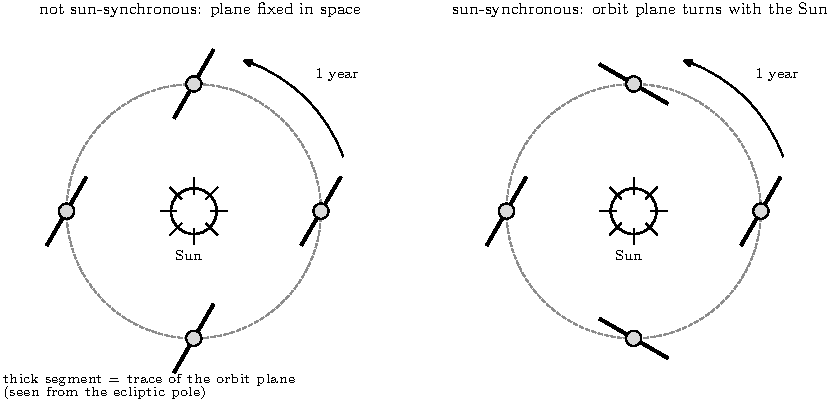
\includegraphics[width=0.85\linewidth]{sso}\end{center}

\paragraph{Perturbation used.} The \textbf{$J_2$ harmonic (Earth oblateness)}. Averaged over one orbit it produces a secular precession
of the node,
\begin{equation}
\langle\dot{\Omega}\rangle=-\frac{3R_{E}^{2}J_{2}\sqrt{\mu_{E}}}{2a^{7/2}(1-e^{2})^{2}}\,c_{i},\qquad
T_{prec}=\frac{2\pi}{|\langle\dot\Omega\rangle|}=\frac{4\pi\,a^{7/2}(1-e^2)^2}{3R_E^2J_2\sqrt{\mu_E}\,|c_i|},
\end{equation}
whose magnitude can be tuned with $a$, $e$, $i$. Sun-synchronism requires $T_{prec}=1$ year \emph{and} the correct sense of rotation:
\begin{equation}
\langle\dot{\Omega}\rangle=+\frac{2\pi}{T_{yr}}\ \Longrightarrow\
i=\arccos\!\left[-\frac{2\pi}{T_{yr}}\,\frac{2\,a^{7/2}(1-e^{2})^{2}}{3R_{E}^{2}J_{2}\sqrt{\mu_{E}}}\right].
\end{equation}

\paragraph{Prograde or retrograde?} \textbf{Retrograde.} The Earth moves around the Sun counter-clockwise as seen from the north
ecliptic pole, so the orbit plane must precess counter-clockwise (eastward): $\langle\dot\Omega\rangle>0$. Since the factor multiplying
$c_i$ is negative, this requires $c_i<0$, i.e.\ $i>\pi/2$. For direct orbits ($i<90^\circ$) $J_2$ makes the node regress westward,
the wrong way. Typical values for circular orbits: $i\simeq97.4^\circ$ at 500\,km, $98.2^\circ$ at 700\,km, $98.6^\circ$ at 800\,km
(near-polar, slightly retrograde); the inclination grows with altitude, and above $a\simeq12\,350$\,km ($c_i=-1$) no sun-synchronous
circular orbit exists \notinnotes (values computed from the formula above). The notes report the plot of altitude vs inclination for $e=0$.

\begin{keyf}
$\langle\dot\Omega\rangle=-\dfrac{3R_E^2J_2\sqrt{\mu_E}}{2a^{7/2}(1-e^2)^2}c_i=+\dfrac{2\pi}{T_{yr}}$ \ $\Rightarrow$ \
$c_i=-\dfrac{2\pi}{T_{yr}}\dfrac{2a^{7/2}(1-e^2)^2}{3R_E^2J_2\sqrt{\mu_E}}<0$ \ $\Rightarrow$ retrograde, $i\approx98^\circ$ in LEO.
\end{keyf}

\pitfalls
\begin{itemize}
\item The sense of precession matters (not only the period): this is what forces $i>90^\circ$.
\item Sun-synchronous is not "geosynchronous" and not "polar": it is slightly retrograde.
\item The perturbation is $J_2$ (oblateness), not the Sun's gravity.
\end{itemize}

\source{cap08.tex l.1029--1062 (precession of the plane), l.1064--1099 (sun-synchronous orbits). Formulario: \fml{8-SSO}.}

% ---------------------------------------------------------------------
\question{C7}{Third-body perturbation: exact acceleration and effect on the angular momentum}
% source: cap08.tex l.1101-1205 (exact), l.1211-1329 (gravity gradient), l.1331-1453 (average effect)
\begin{qbox}
Derive the exact third-body perturbing acceleration and describe how a third-body perturbation affects the angular momentum of
a spacecraft in a circular Earth orbit.
\qmeta{list by chapter ("2025's Q"); Jan 2025 ("physical nature of the third-body perturbation and derivation of the exact acceleration formula").}
\qnote{If only the nature and the exact formula are asked (Jan 2025): write points 1--3 of the outline. Adjacent: \qref{C8}.}
\end{qbox}

\begin{outline}
\begin{enumerate}
\item Physical nature: the third body (Sun, Moon) attracts both the spacecraft and the Earth; the perturbation is the \emph{difference} (tidal).
\item Inertial equations for the spacecraft and for the Earth; subtraction $\Rightarrow$ relative motion = Keplerian + $\underline a_{3B}$.
\item Exact formula $\underline a_{3B}=\mu_2\left[\frac{\underline r_{21}}{r_{21}^3}-\frac{\underline r_{2S}}{r_{2S}^3}\right]=-\mu_2\left\{\frac{\underline r_{12}}{r_{12}^3}+\frac{\underline r_{1S}-\underline r_{12}}{|\underline r_{1S}-\underline r_{12}|^3}\right\}$.
\item Effect on $\underline h$ (circular orbit): gravity gradient, $\dot{\underline h}=\underline r\times\underline f$, double averaging $\Rightarrow$ $\langle\langle\dot{\underline h}\rangle\rangle=\underline\omega_h\times\underline h$: precession about $\hat h_{3B}$, $|\underline h|$ constant.
\end{enumerate}
\end{outline}

\answer
\paragraph{Physical nature.} A spacecraft orbiting the Earth (body 1) is also attracted by other celestial bodies, mainly the Moon
and the Sun (body 2). The Earth itself is accelerated by body 2. What perturbs the motion \emph{relative to the Earth} is the
\textbf{difference} between the attraction of body 2 on the spacecraft and on the Earth (a tidal, differential effect). It is a
conservative, gravitational perturbation; it is small in LEO ($\simeq10^{-7}a_0$ at 1000\,km) and becomes a main perturbation
at high altitude (GEO and above).
\begin{center}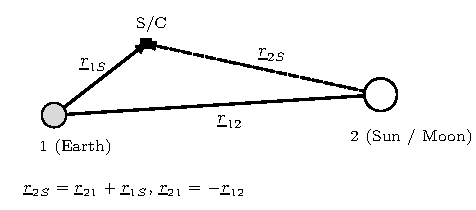
\includegraphics[width=0.48\linewidth]{thirdbody}\end{center}

\paragraph{Derivation of the exact acceleration.} Notation: $\underline r_S$, $\underline r_1$, $\underline r_2$ inertial positions of spacecraft,
Earth and third body; $\underline r_{jS}=\underline r_S-\underline r_j$; $\underline r_{21}=\underline r_1-\underline r_2=-\underline r_{12}$;
$\mu_j$ gravitational parameters. In an inertial frame:
\begin{equation}
\frac{d^{2}\underline{r}_{S}}{dt^{2}}=-\frac{\mu_{1}}{r_{1S}^{3}}\underline{r}_{1S}-\frac{\mu_{2}}{r_{2S}^{3}}\underline{r}_{2S},
\qquad
\frac{d^{2}\underline{r}_{1}}{dt^{2}}=-\frac{\mu_{2}}{r_{21}^{3}}\underline{r}_{21}
\end{equation}
(the spacecraft exerts negligible gravity on the Earth). Subtracting, the motion relative to the Earth, $\underline r_{1S}=\underline r_S-\underline r_1$, obeys
\begin{equation}
\frac{d^{2}\underline{r}_{1S}}{dt^{2}}=-\frac{\mu_{1}}{r_{1S}^{3}}\underline{r}_{1S}
+\underbrace{\left[\frac{\mu_{2}}{r_{21}^{3}}\underline{r}_{21}-\frac{\mu_{2}}{r_{2S}^{3}}\underline{r}_{2S}\right]}_{\underline a_{3B}} .
\end{equation}
With $\underline r_{2S}=\underline r_{21}+\underline r_{1S}=\underline r_{1S}-\underline r_{12}$:
\begin{equation}
\boxed{\;\underline{a}_{3B}=-\mu_{2}\left\{\frac{\underline{r}_{12}}{r_{12}^{3}}
+\frac{\underline{r}_{1S}-\underline{r}_{12}}{\left[(\underline{r}_{1S}-\underline{r}_{12})\cdot(\underline{r}_{1S}-\underline{r}_{12})\right]^{3/2}}\right\}\;}
\end{equation}
The first term is the (indirect) acceleration of the Earth towards body 2, the second the (direct) attraction of body 2 on the
spacecraft. The formula is exact; to use it in the Gauss equations, $\underline r_{12}$ (Moon or Sun position w.r.t.\ the Earth) and
$\underline r_{1S}=\frac{p}{1+ec_{\theta_*}}\hat r$ are projected on $(\hat r,\hat\theta,\hat h)$.

\paragraph{Effect on the angular momentum of a circular orbit.}
\begin{enumerate}
\item Since $r=r_{1S}\ll r_{12}$, the acceleration is approximated by the \textbf{gravity gradient} (\qref{C8}):
$\underline f_{3B}\simeq\frac{\mu_2}{r_{12}^5}\left[3\underline r_{12}\underline r_{12}^T-r_{12}^2\underrightarrow{1}\right]\cdot\underline r$.
\item $\dot{\underline h}=\underline r\times\underline f_{3B}$; the term in $\underrightarrow{1}$ gives $\underline r\times\underline r=\underline 0$:
\begin{equation}
\frac{d\underline h}{dt}=\frac{3\mu_2}{r_{12}^5}(\underline r\times\underline r_{12})(\underline r_{12}\cdot\underline r)=-\frac{3\mu_2}{r_{12}^5}\,\underline r_{12}\times\left(\underline r\,\underline r^T\right)\underline r_{12}.
\end{equation}
\item \textbf{First averaging} over one spacecraft period ($r_{12}$ frozen, $\hat r=\hat Nc_{\theta_t}+\hat Ms_{\theta_t}$ in the orbit plane, $r=R$):
$\langle c^2_{\theta_t}\rangle=\langle s^2_{\theta_t}\rangle=\frac12$, $\langle c_{\theta_t}s_{\theta_t}\rangle=0$ $\Rightarrow$
$\langle\underline r\,\underline r^T\rangle=R^2\left[\frac12\underrightarrow{1}-\frac12\hat h\hat h^T\right]$, hence
$\left\langle\dot{\underline h}\right\rangle=\frac{3\mu_2R^2}{2r_{12}^5}(\underline r_{12}\times\hat h)(\hat h\cdot\underline r_{12})$.
\item \textbf{Second averaging} over one period of the perturbing body (circular relative orbit with normal $\hat h_{3B}$):
$\langle\underline r_{12}\underline r_{12}^T\rangle=r_{12}^2\left[\frac12\underrightarrow{1}-\frac12\hat h_{3B}\hat h_{3B}^T\right]$, which gives
\begin{equation}
\left\langle\!\left\langle\frac{d\underline{h}}{dt}\right\rangle\!\right\rangle=\underline\omega_h\times\underline h,\qquad
\underline{\omega}_{h}=-\frac{3}{4}\frac{\mu_{2}R^{2}}{r_{12}^{3}\,h}\left(\hat{h}\cdot\hat{h}_{3B}\right)\hat{h}_{3B},\qquad h=\sqrt{\mu_1R}.
\end{equation}
\end{enumerate}
\textbf{Result}: on average $\underline h$ only \textbf{rotates} about $\hat h_{3B}$ (normal to the orbit of the third body: ecliptic pole for the Sun),
\textbf{its magnitude does not change} (orbit size unchanged, $\dot{\underline h}\perp\underline h$), while the orbit plane precesses with
period $T_{prec}=2\pi/|\underline\omega_h|$; clockwise if $\hat h\cdot\hat h_{3B}>0$, counter-clockwise if $<0$. The inclination with respect to
the third body's orbit plane stays constant on average.
Example: the Moon, regarded as an Earth satellite perturbed by the Sun ($\hat h_{3B}$ = ecliptic pole): its node regresses with
$T_{prec}\simeq18$ years.

\begin{keyf}
$\underline a_{3B}=\mu_2\left[\dfrac{\underline r_{21}}{r_{21}^3}-\dfrac{\underline r_{2S}}{r_{2S}^3}\right]$, $\underline r_{2S}=\underline r_{21}+\underline r_{1S}$; \
$\dot{\underline h}=\underline r\times\underline f$; \ $\langle\langle\dot{\underline h}\rangle\rangle=\underline\omega_h\times\underline h$, \
$\underline\omega_h=-\dfrac34\dfrac{\mu_2R^2}{r_{12}^3h}(\hat h\cdot\hat h_{3B})\hat h_{3B}$.
\end{keyf}

\pitfalls
\begin{itemize}
\item The perturbation is the \emph{difference} of the two attractions (spacecraft minus Earth), not the attraction on the spacecraft alone.
\item Write the inertial equations for both bodies and subtract; keep track of $\underline r_{21}=-\underline r_{12}$.
\item The average effect is a precession of $\underline h$ at constant magnitude.
\end{itemize}

\source{cap08.tex l.1101--1205 (exact acceleration), l.1211--1329 (gravity gradient), l.1331--1453 (average effect on circular orbits;
errata \#14--15), l.1455--1470 (Moon). Formulario: \fml{8-3BA}, \fml{8-MOO}.}

% ---------------------------------------------------------------------
\question{C8}{Gravity-gradient dyadic from the third-body acceleration}
% source: cap08.tex l.1211-1329
\begin{qbox}
Prove the gravity-gradient dyadic starting from the third-body perturbing-force formula
\[
\underline f_{3B}=-\frac{\mu_S}{r_{2S}^3}\left(\underline r_{21}+\underline r_{1S}\right)+\frac{\mu_S}{r_{21}^3}\,\underline r_{21},
\]
while specifying the fundamental condition needed to obtain it.
\qmeta{$\times$2 in the list (2025); Feb 2025; Sep 2025.}
\qnote{Here body 2 is the Sun ($\mu_2=\mu_S$). Adjacent: \qref{C7}.}
\end{qbox}

\begin{outline}
\begin{enumerate}
\item Write $\underline f_{3B}=\underline g(\underline r_{21}+\underline r_{1S})-\underline g(\underline r_{21})$ with $\underline g(\underline x)=-\mu_2\underline x/x^3$.
\item Fundamental condition: $|\underline r_{1S}|\ll|\underline r_{21}|$ (spacecraft much closer to the Earth than the third body).
\item First-order Taylor expansion about $\underline r_{21}$: $\underline f_{3B}\simeq\left.\frac{\partial\underline g}{\partial\underline x}\right|_{\underline r_{21}}\cdot\underline r_{1S}$ (a dyad).
\item Components: $\partial_j(-\mu_2x_i/x^3)=-\mu_2\delta_{ij}/x^3+3\mu_2x_ix_j/x^5$ (show (1,1) and (1,2)).
\item Compact form $\frac{\mu_2}{r_{12}^5}\left[3\underline r_{12}\underline r_{12}-r_{12}^2\underrightarrow{1}\right]$; final $\underline f_{3B}$; interpretation (tidal stretching).
\end{enumerate}
\end{outline}

\answer
\paragraph{Starting point.} With $\underline r_{2S}=\underline r_{21}+\underline r_{1S}$ the third-body acceleration is the difference of the
gravitational field of body 2,
\begin{equation}
\underline g(\underline x):=-\frac{\mu_2}{x^3}\underline x,\qquad
\underline f_{3B}=-\frac{\mu_2}{r_{2S}^3}\underline r_{2S}-\left(-\frac{\mu_2}{r_{21}^3}\underline r_{21}\right)
=\underline g(\underline r_{21}+\underline r_{1S})-\underline g(\underline r_{21}),
\end{equation}
evaluated at the spacecraft ($\underline x=\underline r_{2S}$) and at the Earth ($\underline x=\underline r_{21}$).

\paragraph{Fundamental condition.}
\begin{equation}
\boxed{\;|\underline r_{1S}|\ll|\underline r_{21}|\;}
\end{equation}
the distance of the spacecraft from the Earth is much smaller than the distance of the third body from the Earth (usually satisfied:
LEO--GEO radii $\ll$ 384\,400\,km or 1\,AU). Then $\underline r_{1S}$ is a small displacement from $\underline r_{21}$ and a first-order Taylor
expansion is accurate:
\begin{equation}
\underline f_{3B}\simeq\left.\frac{\partial}{\partial\underline r_{2j}}\left[-\frac{\mu_2}{r_{2j}^3}\underline r_{2j}\right]\right|_{\underline r_{21}}\!\cdot\underline r_{1S}.
\end{equation}

\paragraph{The gravity-gradient dyad.} The gradient of a vector field with respect to a position vector is a dyad (second-order tensor),
which acting on a vector gives a vector. In an orthonormal basis $\{\hat c_1,\hat c_2,\hat c_3\}$, with $\underline r_{2j}=x\hat c_1+y\hat c_2+z\hat c_3$:
\begin{equation}
\underrightarrow{D}=[\hat c_1\ \hat c_2\ \hat c_3]
\begin{bmatrix}
\partial_x\!\left(-\frac{\mu_2x}{r_{2j}^3}\right)&\partial_y\!\left(-\frac{\mu_2x}{r_{2j}^3}\right)&\partial_z\!\left(-\frac{\mu_2x}{r_{2j}^3}\right)\\[3pt]
\partial_x\!\left(-\frac{\mu_2y}{r_{2j}^3}\right)&\partial_y\!\left(-\frac{\mu_2y}{r_{2j}^3}\right)&\partial_z\!\left(-\frac{\mu_2y}{r_{2j}^3}\right)\\[3pt]
\partial_x\!\left(-\frac{\mu_2z}{r_{2j}^3}\right)&\partial_y\!\left(-\frac{\mu_2z}{r_{2j}^3}\right)&\partial_z\!\left(-\frac{\mu_2z}{r_{2j}^3}\right)
\end{bmatrix}
\begin{bmatrix}\hat c_1\\ \hat c_2\\ \hat c_3\end{bmatrix},\qquad r_{2j}=\sqrt{x^2+y^2+z^2}.
\end{equation}
Using $\partial r_{2j}/\partial x=x/r_{2j}$:
\begin{equation}
D_{11}=\frac{\partial}{\partial x}\left(-\frac{\mu_2x}{(x^2+y^2+z^2)^{3/2}}\right)=-\frac{\mu_2}{r_{12}^3}+\frac{3\mu_2x^2}{r_{12}^5},\qquad
D_{12}=\frac{\partial}{\partial y}\left(-\frac{\mu_2x}{(x^2+y^2+z^2)^{3/2}}\right)=\frac{3\mu_2xy}{r_{12}^5},
\end{equation}
and in general
\begin{equation}
D_{ij}=-\frac{\mu_2}{r_{12}^3}\,\delta_{ij}+\frac{3\mu_2\,x_ix_j}{r_{12}^5}.
\end{equation}
The derivatives are evaluated at $\underline r_{21}$; since each $D_{ij}$ is even in the coordinates and $r_{21}=r_{12}$, the result is the same
at $\underline r_{21}=-\underline r_{12}$. In coordinate-free form:
\begin{equation}
\boxed{\;\underrightarrow{D}=\left.\frac{\partial}{\partial\underline r_{2j}}\left[-\frac{\mu_2}{r_{2j}^3}\underline r_{2j}\right]\right|_{\underline r_{21}}
=\frac{\mu_{2}}{r_{12}^{5}}\left[3\,\underline{r}_{12}\underline{r}_{12}-r_{12}^{2}\,\underrightarrow{1}\right]\;}
\qquad \underrightarrow{1}=\hat c_1\hat c_1+\hat c_2\hat c_2+\hat c_3\hat c_3 ,
\end{equation}
where $\underline r_{12}\underline r_{12}$ ($=\underline r_{12}\underline r_{12}^T$) is the outer product. Therefore
\begin{equation}
\underline f_{3B}\simeq\frac{\mu_2}{r_{12}^5}\left[3\,\underline r_{12}\,(\underline r_{12}\cdot\underline r_{1S})-r_{12}^2\,\underline r_{1S}\right]
=\frac{\mu_2}{r_{12}^3}\left[3\,\hat r_{12}(\hat r_{12}\cdot\underline r_{1S})-\underline r_{1S}\right].
\end{equation}

\paragraph{Interpretation.} The perturbation is linear in $r_{1S}$ and proportional to $\mu_2/r_{12}^3$ (tidal acceleration). In a frame with
the first axis along $\hat r_{12}$ the dyad is $\frac{\mu_2}{r_{12}^3}\mathrm{diag}(2,-1,-1)$: the spacecraft is pulled away from the Earth along
the Earth--third-body line (stretching, $+2$) and pushed towards it in the transverse directions (compression, $-1$). Because of
the $1/r_{12}^3$ factor the Moon, though much less massive, has a tidal effect about twice that of the Sun \notinnotes. This form is
used to compute the average effect on $\underline h$ (\qref{C7}).

\begin{keyf}
Condition $r_{1S}\ll r_{21}$; \ $\underline f_{3B}\simeq\dfrac{\partial\underline g}{\partial\underline x}\Big|_{\underline r_{21}}\!\cdot\underline r_{1S}$; \
$D_{ij}=-\dfrac{\mu_2}{r^3}\delta_{ij}+\dfrac{3\mu_2x_ix_j}{r^5}$; \ $\underrightarrow{D}=\dfrac{\mu_2}{r_{12}^5}\left[3\underline r_{12}\underline r_{12}-r_{12}^2\underrightarrow{1}\right]$.
\end{keyf}

\pitfalls
\begin{itemize}
\item State the condition $|\underline r_{1S}|\ll|\underline r_{21}|$ before expanding: it is what the question asks explicitly.
\item The zero-order term $\underline g(\underline r_{21})$ cancels with the second term of $\underline f_{3B}$: only the gradient survives.
\item Show at least one diagonal and one off-diagonal derivative, then the compact form with the unit dyad.
\end{itemize}

\source{cap08.tex l.1211--1329 (approximate perturbing acceleration using the gravity gradient; the dyad and its compact form).}

% ---------------------------------------------------------------------
\question{C9}{Aerodynamic drag: acceleration and effect on the orbit elements}
% source: cap08.tex l.398-559
\begin{qbox}
Report the expression of the drag acceleration and describe its effect on two specific orbit elements.
\qmeta{Jul 2025; Mar 2025 ("aerodynamic drag").}
\end{qbox}

\begin{outline}
\begin{enumerate}
\item Where it matters (100--1000\,km), exponential atmosphere $\rho(\tilde h)$.
\item $\underline a_D=-\frac12C_D\frac{S}{m}\rho v_R^2\hat v_R$, meaning of each term; $\underline v_R=\underline v-\underline\omega_E\times\underline r$; ballistic coefficient $C_DS/m$.
\item Effect: dissipative, along $-\hat v$ ($f_\theta<0$, $f_h\simeq0$) $\Rightarrow$ $a\downarrow$ and $e\downarrow$ (Gauss equations).
\item Elliptic orbit: drag concentrated at perigee $\Rightarrow$ apogee decreases, circularisation; circular orbit: slow spiral.
\item Near-circular: $\dot a=-C_D\frac Sm\rho\sqrt{\mu a}$, $\sqrt{a_f}-\sqrt{a_i}=-\frac{C_DS}{2m}\rho\sqrt\mu\,\Delta t$. Plane nearly unchanged.
\end{enumerate}
\end{outline}

\answer
\paragraph{When drag matters.} By convention space begins at 100\,km (over 99.9999\% of the atmosphere is below it), but up to about
1000\,km the residual atmosphere still perturbs the orbit, and the effect grows rapidly as the altitude decreases. The density is
modelled with a piecewise exponential law (data from USSA76):
\begin{equation}
\rho(\tilde{h})=\rho_{R,i}\exp\!\left[-\frac{\tilde{h}-\tilde{h}_{R,i}}{H_{R,i}}\right],
\end{equation}
$\tilde h_{R,i}$ reference altitude with density $\rho_{R,i}$, $H_{R,i}$ scale height.

\paragraph{Drag acceleration.}
\begin{equation}
\boxed{\;\underline{a}_{D}=\frac{\underline{D}}{m}=-\frac{1}{2}\,C_{D}\,\frac{S}{m}\,\rho\,v_{R}^{2}\,\hat{v}_{R}\;}
\end{equation}
\begin{itemize}
\item $S$ = aerodynamic reference surface (depends on geometry and attitude); $m$ = spacecraft mass (varies if propulsion is used);
\item $C_D$ = drag coefficient: in the rarefied (free-molecular) regime $C_D\simeq2.2$ (minimum 2 for a sphere);
\item $\rho$ = atmospheric density at the current altitude;
\item $\underline v_R=\underline v-\underline v_a$ = velocity relative to the atmosphere, which is assumed to rotate with the Earth:
$\underline v_a=\underline\omega_E\times\underline r=\omega_Er\cos\phi\,\hat E$ (small compared with the orbital speed).
\end{itemize}
$C_D\,S/m$ is the \textbf{ballistic coefficient}: the larger it is, the stronger the action of drag. Drag is \textbf{dissipative}
(non-conservative, a surface perturbation) and opposite to the relative velocity: essentially $f_\theta<0$, small $f_r$, and
$f_h\simeq0$.

\paragraph{Effect on the elements: $a$ and $e$ decrease.} From the Gauss equations
$\dot a=\frac{2a^2}{h}\left(e\,s_{\theta_*}f_r+\frac pr f_\theta\right)$ and
$\dot e=\sqrt{p/\mu}\left[f_rs_{\theta_*}+f_\theta\frac{e+ec_{\theta_*}^2+2c_{\theta_*}}{1+ec_{\theta_*}}\right]$: with $f_\theta<0$ we get
$\dot a<0$; near perigee ($\theta_*\simeq0$) $\dot e\simeq2\sqrt{p/\mu}\,f_\theta<0$.
\begin{itemize}
\item \textbf{Elliptic orbit}: the density is much higher at perigee, so the drag action is \textbf{concentrated at perigee}. Like a small
retro-burn at perigee, it lowers the \textbf{apogee} altitude, while the perigee altitude is only marginally reduced. Hence
\textbf{$a\downarrow$ (semi-major axis) and $e\downarrow$ (eccentricity)}: the orbit is progressively circularised.
\item \textbf{Circular LEO}: the long-term effect is a \textbf{spiral trajectory slowly decreasing in altitude}, until re-entry.
\item The orbit plane is practically unaffected: $f_h^{(D)}$ is very small, so $\dot i\simeq0$, $\dot\Omega\simeq0$.
\end{itemize}
\begin{center}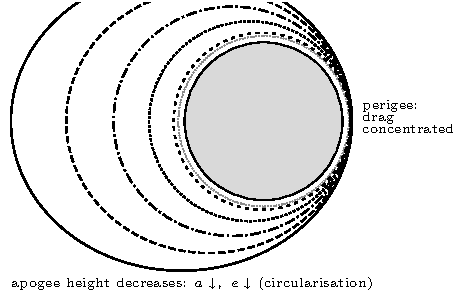
\includegraphics[width=0.45\linewidth]{drag}\end{center}

\paragraph{Approximate analysis for near-circular orbits.} With $a\simeq R$, $v\simeq\sqrt{\mu/a}\,\hat\theta$ and $\underline v_R\simeq\underline v$:
$f_\theta^{(D)}=-\frac12C_D\frac Sm\rho\frac\mu a$, $f_r=f_h=0$, hence
\begin{equation}
\dot{a}=\frac{2a^{3/2}}{\sqrt{\mu}}f_{\theta}^{(D)}=-C_{D}\frac{S}{m}\rho\sqrt{\mu a}
\;\xrightarrow{\ \rho\simeq\text{const}\ }\;
a_{\text{fin}}^{1/2}-a_{\text{ini}}^{1/2}=-\frac{C_{D}S}{2m}\rho\sqrt{\mu}\,(t_{\text{fin}}-t_{\text{ini}}),
\end{equation}
valid for small variations of $a$ (otherwise $\rho$ changes). Note that as $a$ decreases the orbital speed $\sqrt{\mu/a}$ \emph{increases}:
drag removes energy but the satellite speeds up while spiralling down \notinnotes.

\begin{keyf}
$\underline a_D=-\frac12C_D\dfrac Sm\rho v_R^2\hat v_R$, \ $\underline v_R=\underline v-\underline\omega_E\times\underline r$, \ ballistic coeff.\ $C_DS/m$, \
$a\downarrow$, $e\downarrow$; \ $\dot a=-C_D\dfrac Sm\rho\sqrt{\mu a}$.
\end{keyf}

\pitfalls
\begin{itemize}
\item Use the velocity \emph{relative to the atmosphere} and the square of its magnitude.
\item The two elements are $a$ and $e$: explain the perigee mechanism (apogee lowers $\Rightarrow$ circularisation).
\item Drag hardly changes $i$ and $\Omega$.
\end{itemize}

\source{cap08.tex l.398--426 (atmosphere model), l.428--499 (drag acceleration), l.501--519 (effect on elements), l.521--559
(near-circular orbits; errata \#11); Gauss equations l.338--372. Formulario: \fml{8-DRG}, \fml{8-DRC}.}

% =====================================================================
% Group D -- Fundamentals of attitude dynamics, chapters 9-11 (one question per exam)
% Source: latex_notes/SFM_09_*/cap09.tex, SFM_11_*/cap11.tex
% =====================================================================
\qgroup{D}{Attitude dynamics -- Chapters 9 and 11}

One question per exam is on attitude (25\% of the course). Notation of the notes: inertial axes $(\hat E_1,\hat E_2,\hat E_3)$,
body axes $(\hat e_1,\hat e_2,\hat e_3)$, rotation matrix $\underset{B\leftarrow N}{\underline{\underline R}}$ such that
$[\hat e_1\ \hat e_2\ \hat e_3]^T=\underset{B\leftarrow N}{\underline{\underline R}}\,[\hat E_1\ \hat E_2\ \hat E_3]^T$. Elementary rotations:
\begin{equation*}
\underline{\underline R}_1(\alpha)=\begin{bmatrix}1&0&0\\0&c_\alpha&s_\alpha\\0&-s_\alpha&c_\alpha\end{bmatrix},\quad
\underline{\underline R}_2(\alpha)=\begin{bmatrix}c_\alpha&0&-s_\alpha\\0&1&0\\s_\alpha&0&c_\alpha\end{bmatrix},\quad
\underline{\underline R}_3(\alpha)=\begin{bmatrix}c_\alpha&s_\alpha&0\\-s_\alpha&c_\alpha&0\\0&0&1\end{bmatrix}.
\end{equation*}
For the singularities of the angle sequences the explicit full rotation matrices are not requested (course program).

\begin{center}
\small
\begin{tabular}{@{}lllr@{}}
\toprule
Q & Topic & Asked & Page\\
\midrule
\ref{q:D1} & Bryant angles (3-2-1) & Jan 2023 & \pageref{q:D1}\\
\ref{q:D2} & Euler angles (3-1-3), illustration & list, Mar 2025 & \pageref{q:D2}\\
\ref{q:D3} & Angle sequences vs Euler parameters: pros and cons & list & \pageref{q:D3}\\
\ref{q:D4} & Euler parameters: definition and properties & $\times$2, Sep 2025 & \pageref{q:D4}\\
\ref{q:D5} & Euler parameters: definition and advantages & list & \pageref{q:D5}\\
\ref{q:D6} & Parallel axis theorem & Jul 2025 & \pageref{q:D6}\\
\ref{q:D7} & Inertia dyad, inertia matrix in two frames & $\times$2, Jan 2025, Sep 2024 & \pageref{q:D7}\\
\ref{q:D8} & Torque-free equilibria, no dissipation & $\times$2, Feb 2025 & \pageref{q:D8}\\
\ref{q:D9} & Torque-free equilibria, with dissipation & Jun 2025 & \pageref{q:D9}\\
\bottomrule
\end{tabular}
\end{center}

% ---------------------------------------------------------------------
\question{D1}{Bryant angles}
% source: cap09.tex l.207-212, l.258-305, l.390-424 (kinematics)
\begin{qbox}
List the Bryant angles, give their names, the intervals of definition, and the associated sequence of elementary rotations
(inertial $\to$ body frame).
\qmeta{Jan 2023.}
\qnote{Adjacent: \qref{D2} (Euler angles, 3-1-3).}
\end{qbox}

\begin{outline}
\begin{enumerate}
\item Attitude = orientation of body axes w.r.t.\ inertial axes; only 3 of the 9 elements of $\underline{\underline R}$ are independent $\Rightarrow$ 3 angles.
\item Bryant (3-2-1): $\underset{B\leftarrow N}{\underline{\underline R}}=\underline{\underline R}_1(\phi)\underline{\underline R}_2(\theta)\underline{\underline R}_3(\psi)$.
\item Names and intervals: $\psi$ yaw $[-\pi,\pi[$, $\theta$ pitch $[-\pi/2,\pi/2]$, $\phi$ roll $[-\pi,\pi[$.
\item Sequence: yaw about $\hat E_3$, pitch about the new axis 2, roll about the final axis 1 (sketch).
\item Aircraft meaning of the axes; singularity $\theta=\pm\pi/2$.
\end{enumerate}
\end{outline}

\answer
\paragraph{Why three angles.} The attitude of the body axes $(\hat e_1,\hat e_2,\hat e_3)$ with respect to the inertial axes $(\hat E_1,\hat E_2,\hat E_3)$
is described by the rotation matrix $\underset{B\leftarrow N}{\underline{\underline R}}$, with 9 elements linked by 6 orthonormality relations:
only 3 are independent. Three angles, associated with three distinct and subsequent elementary rotations, are therefore a minimal
representation (in each sequence the order of the rotations matters).

\paragraph{Bryant angles (sequence 3-2-1).}
\begin{equation}
\underset{B\leftarrow N}{\underline{\underline{R}}}=\underline{\underline{R}}_{1}(\phi)\,\underline{\underline{R}}_{2}(\theta)\,\underline{\underline{R}}_{3}(\psi)
\end{equation}
\begin{center}
\small
\begin{tabular}{@{}llll@{}}
\toprule
angle & name & rotation about & interval\\
\midrule
$\psi$ & yaw & axis 3 of the inertial frame, $\hat E_3$ & $[-\pi,\pi[$\\
$\theta$ & pitch & intermediate axis 2, $\hat\jmath$ & $[-\pi/2,\pi/2]$\\
$\phi$ & roll & body axis 1, $\hat e_1$ & $[-\pi,\pi[$\\
\bottomrule
\end{tabular}
\end{center}

\paragraph{Sequence of elementary rotations (inertial $\to$ body).}
\begin{enumerate}
\item \textbf{Yaw}: rotation by $\psi$ about $\hat E_3$: $(\hat E_1,\hat E_2,\hat E_3)\to(\hat\imath,\hat\jmath,\hat E_3)$, with
$\hat\jmath=-s_\psi\hat E_1+c_\psi\hat E_2$;
\item \textbf{Pitch}: rotation by $\theta$ about the new axis 2, $\hat\jmath$: $(\hat\imath,\hat\jmath,\hat E_3)\to(\hat e_1,\hat\jmath,\hat k'')$;
\item \textbf{Roll}: rotation by $\phi$ about the new axis 1, $\hat e_1$: $(\hat e_1,\hat\jmath,\hat k'')\to(\hat e_1,\hat e_2,\hat e_3)$.
\end{enumerate}
The matrices are multiplied right to left: the first rotation ($\underline{\underline R}_3(\psi)$) is the rightmost.
\begin{center}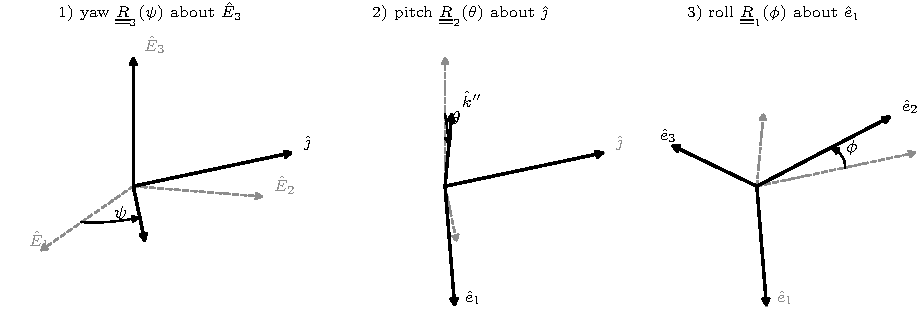
\includegraphics[width=0.95\linewidth]{bryant321}\\
{\footnotesize Grey dashed: frame before each rotation; black: frame after. Computed with $\psi=40^\circ$, $\theta=\phi=35^\circ$.}\end{center}

\paragraph{Use and meaning.} Widely used in atmospheric flight, especially for aircraft: $\hat e_1$ = longitudinal axis, $\hat e_2$ = right wing,
$\hat e_3$ = downward direction (in usual flight). A natural choice of reference is $\hat E_1=\hat N_L$ (local North), $\hat E_2=\hat E_L$ (East),
$\hat E_3=-\hat r_L$ (local downward): for small angles the body axes are close to the reference ones, and yaw, pitch, roll have
the familiar meaning of heading, nose up/down and bank.

\paragraph{Uniqueness and singularity.} With these intervals every orientation corresponds to a unique set $(\psi,\theta,\phi)$, \emph{except}
for $\theta=\pm\pi/2$: then the first and third rotation axes coincide and only $\psi-\phi$ (or $\psi+\phi$) is defined ("gimbal lock").
The kinematic equations $\dot\psi=(s_\phi\omega_2+c_\phi\omega_3)/c_\theta$, $\dot\phi=\omega_1+\tan\theta(s_\phi\omega_2+c_\phi\omega_3)$ are
singular at the same values. The angles are recovered from the matrix as $\theta=-\arcsin(r_{13})$,
$\phi=\mathrm{atan2}(r_{23},r_{33})$, $\psi=\mathrm{atan2}(r_{12},r_{11})$.

\begin{fig2draw}
Three small triads. (1) $\hat E_1,\hat E_2,\hat E_3$ dashed, rotate the first two by $\psi$ around $\hat E_3$. (2) Around the new $\hat\jmath$
tilt axis 1 by $\theta$ (pitch). (3) Around the new axis $\hat e_1$ rotate axes 2--3 by $\phi$ (roll). Write the intervals under each angle.
\end{fig2draw}

\begin{keyf}
$\underset{B\leftarrow N}{\underline{\underline R}}=\underline{\underline R}_1(\phi)\underline{\underline R}_2(\theta)\underline{\underline R}_3(\psi)$; \
yaw $\psi\in[-\pi,\pi[$, pitch $\theta\in[-\frac\pi2,\frac\pi2]$, roll $\phi\in[-\pi,\pi[$; \ singular at $\theta=\pm\pi/2$.
\end{keyf}

\pitfalls
\begin{itemize}
\item Order: 3 (yaw) first, then 2 (pitch), then 1 (roll); in the product the first rotation is on the right.
\item Pitch is limited to $[-\pi/2,\pi/2]$ (not $[0,\pi]$ like the Euler nutation angle).
\item Each rotation is about an axis of the \emph{current} (intermediate) frame.
\end{itemize}

\source{cap09.tex l.207--212 (sequences of angles), l.258--305 (Bryant angles, singularity, angles from $\underline{\underline R}$), l.390--424 (kinematics). Formulario: \fml{9-321}, \fml{9-K21}.}

% ---------------------------------------------------------------------
\question{D2}{Euler angles (3-1-3)}
% source: cap09.tex l.207-256, l.319-388
\begin{qbox}
Define the Euler angles (names and rotation sequence) and specify their ranges of definition. Provide a geometric illustration.
\qmeta{list by chapter (Ch.\,9); Mar 2025 ("Euler angles").}
\qnote{Adjacent: \qref{D1} (Bryant angles, 3-2-1).}
\end{qbox}

\begin{outline}
\begin{enumerate}
\item 3 independent parameters in $\underline{\underline R}$ $\Rightarrow$ 3 elementary rotations.
\item $\underset{B\leftarrow N}{\underline{\underline R}}=\underline{\underline R}_3(\phi)\underline{\underline R}_1(\theta)\underline{\underline R}_3(\psi)$.
\item $\psi$ precession $[-\pi,\pi[$, $\theta$ nutation $[0,\pi]$, $\phi$ spin $[-\pi,\pi[$.
\item Sequence with the line of nodes $\hat\imath$; illustration.
\item Singularity $\theta=0,\pi$ (only $\psi\pm\phi$ defined); kinematic equations singular; typical use (spinning bodies).
\end{enumerate}
\end{outline}

\answer
\paragraph{Definition.} Since only 3 of the 9 direction cosines are independent, the attitude can be described by three angles,
associated with three subsequent elementary rotations. The Euler angles use the sequence \textbf{3-1-3}:
\begin{equation}
\underset{B\leftarrow N}{\underline{\underline{R}}}=\underline{\underline{R}}_{3}(\phi)\,\underline{\underline{R}}_{1}(\theta)\,\underline{\underline{R}}_{3}(\psi)
\end{equation}
\begin{center}
\small
\begin{tabular}{@{}llll@{}}
\toprule
angle & name & rotation about & range\\
\midrule
$\psi$ & precession & $\hat E_3$ & $[-\pi,\pi[$\\
$\theta$ & nutation & line of nodes $\hat\imath$ (new axis 1) & $[0,\pi]$\\
$\phi$ & spin & body axis $\hat e_3$ & $[-\pi,\pi[$\\
\bottomrule
\end{tabular}
\end{center}

\paragraph{Sequence (inertial $\to$ body).}
\begin{enumerate}
\item rotation $\psi$ about $\hat E_3$: $\hat E_1\to\hat\imath=c_\psi\hat E_1+s_\psi\hat E_2$ (the \emph{line of nodes}, intersection of the planes
$\hat E_1\hat E_2$ and $\hat e_1\hat e_2$);
\item rotation $\theta$ about $\hat\imath$: $\hat E_3$ tilts to $\hat e_3$; $\theta$ is the angle between $\hat E_3$ and $\hat e_3$;
\item rotation $\phi$ about $\hat e_3$: the axes $\hat e_1$, $\hat e_2$ are obtained; $\phi$ is measured from the line of nodes to $\hat e_1$.
\end{enumerate}
\begin{center}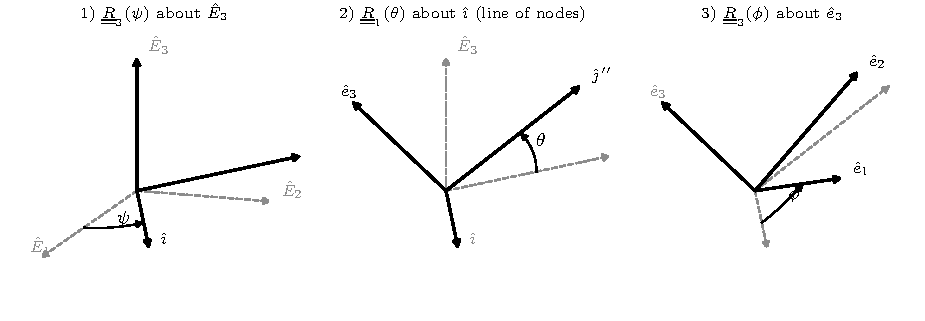
\includegraphics[width=0.95\linewidth]{euler313}\\
{\footnotesize Geometric illustration, one rotation per panel (grey dashed: before; black: after); $\psi=40^\circ$, $\theta=\phi=35^\circ$.}\end{center}
Geometric meaning: $\psi$ and $\theta$ fix the direction of the body axis $\hat e_3$ (like longitude of the node and inclination), $\phi$ the
rotation of the body about it. The same sequence relates the ECI frame to the orbital frame with $(\Omega,i,\theta_t)$
($\underline{\underline R}_3(\theta_t)\underline{\underline R}_1(i)\underline{\underline R}_3(\Omega)$).

\paragraph{Uniqueness and singularities.} With these ranges every orientation corresponds to a unique $(\psi,\theta,\phi)$, except for
$\theta=0$ and $\theta=\pi$: then $\hat e_3=\pm\hat E_3$, the two rotations about axis 3 are about the same axis and only $\psi+\phi$
(or $\psi-\phi$) is meaningful; e.g.\ for $\theta=0$, $\underline{\underline R}=\underline{\underline R}_3(\psi+\phi)$. The kinematic equations
\begin{equation}
\dot\psi=\frac{s_\phi\omega_1+c_\phi\omega_2}{s_\theta},\qquad \dot\theta=c_\phi\omega_1-s_\phi\omega_2,\qquad
\dot\phi=\omega_3-\frac{s_\phi\omega_1+c_\phi\omega_2}{\tan\theta}
\end{equation}
are nonlinear and singular at the same values. Angles from the matrix: $\theta=\arccos r_{33}$, $\phi=\mathrm{atan2}(r_{13},r_{23})$,
$\psi=\mathrm{atan2}(r_{31},-r_{32})$. Euler angles are natural for spinning, axisymmetric spacecraft (torque-free motion:
precession and spin rates).

\begin{fig2draw}
Inertial triad; the line of nodes $\hat\imath$ in the $\hat E_1\hat E_2$ plane at angle $\psi$ from $\hat E_1$; the body axis $\hat e_3$ tilted by $\theta$
from $\hat E_3$ (rotation about $\hat\imath$); $\hat e_1$ in the body plane at angle $\phi$ from $\hat\imath$.
\end{fig2draw}

\begin{keyf}
$\underset{B\leftarrow N}{\underline{\underline R}}=\underline{\underline R}_3(\phi)\underline{\underline R}_1(\theta)\underline{\underline R}_3(\psi)$; \
precession $\psi\in[-\pi,\pi[$, nutation $\theta\in[0,\pi]$, spin $\phi\in[-\pi,\pi[$; \ singular at $\theta=0,\pi$.
\end{keyf}

\pitfalls
\begin{itemize}
\item The middle rotation is about axis 1 (line of nodes), and the first and third are both about "axis 3" (of different frames).
\item Nutation in $[0,\pi]$, not $[-\pi/2,\pi/2]$.
\end{itemize}

\source{cap09.tex l.207--256 (Euler angles, singularities, angles from $\underline{\underline R}$), l.319--388 (kinematics). Formulario: \fml{9-313}, \fml{9-K13}.}

% ---------------------------------------------------------------------
\question{D3}{Angle sequences vs Euler parameters (quaternions): pros and cons}
% source: cap09.tex l.207-212, 319-424, 681-892
\begin{qbox}
In attitude kinematics, list and describe the main pros and cons of using angle sequences versus Euler parameters (quaternions).
\qmeta{list by chapter (Ch.\,9).}
\qnote{Adjacent: \qref{D4}, \qref{D5} (definition of quaternions).}
\end{qbox}

\begin{outline}
\begin{enumerate}
\item The two representations: three angles (e.g.\ 3-1-3, 3-2-1) vs $\{q_0,\underline q\}$ from principal axis and angle.
\item Number of parameters and redundancy (3, 0 vs 4, 1).
\item Intuitiveness.
\item Singularities (representation and kinematic equations) vs none.
\item Kinematic equations: nonlinear (trigonometric) vs bilinear; computational cost.
\item Relative attitude/misalignment: simple error quaternion $\{q_{0,e},\underline q_e\}$. Summary table.
\end{enumerate}
\end{outline}

\answer
\paragraph{The two representations.}
\begin{itemize}
\item \textbf{Sequences of angles}: three elementary rotations, e.g.\ Euler 3-1-3 $\underline{\underline R}_3(\phi)\underline{\underline R}_1(\theta)\underline{\underline R}_3(\psi)$ or
Bryant 3-2-1 $\underline{\underline R}_1(\phi)\underline{\underline R}_2(\theta)\underline{\underline R}_3(\psi)$.
\item \textbf{Euler parameters (quaternions)}: from Euler's theorem (single rotation $\Phi$ about the eigen-axis $\hat a$):
$q_0=\cos\frac\Phi2$, $\underline q=\hat a\sin\frac\Phi2$, with $q_0^2+q_1^2+q_2^2+q_3^2=1$.
\end{itemize}

\paragraph{Comparison.}
\begin{center}
\small
\begin{tabular}{@{}p{3.0cm}p{5.8cm}p{5.8cm}@{}}
\toprule
 & Sequences of angles & Quaternions (Euler parameters)\\
\midrule
number of parameters & 3 (minimal), redundancy 0 & 4, one constraint $\Rightarrow$ redundancy 1\\
intuitiveness & intuitive (yaw, pitch, roll; precession, nutation, spin) & less intuitive (axis and half-angle)\\
singularities & 2 values of the intermediate angle ($\theta=0,\pi$ for 3-1-3, $\pm\pi/2$ for 3-2-1) & singularity-free\\
kinematic equations & singular at the same values; nonlinear (trigonometric, divisions by $s_\theta$ or $c_\theta$): expensive & no singularity; bilinear in $(q,\underline\omega)$: $\dot q_0=-\frac12\underline\omega^T\underline q$, $\dot{\underline q}=\frac12(q_0\underline\omega-\tilde\omega\underline q)$: cheap\\
rotation matrix & products of sines and cosines & quadratic polynomial in $q_i$ (no trigonometric functions)\\
relative attitude / misalignment & not clearly measurable & simple: error quaternion $\{q_{0,e},\underline q_e\}$ by quaternion algebra\\
uniqueness & unique within the intervals (except singularities) & two quaternions $\pm q$ for each attitude\\
\bottomrule
\end{tabular}
\end{center}

\paragraph{Discussion.}
\begin{itemize}
\item \textbf{Pros of angles}: minimal set (no constraint to enforce), clear physical meaning, convenient for small-angle analyses, for
pointing requirements and for torque-free spinning bodies.
\item \textbf{Cons of angles}: any three-parameter set has singular orientations (with 3 angles singularities always occur); near them the
kinematic equations blow up ($1/s_\theta$, $1/c_\theta$), so they are unsuitable for large-angle or all-attitude manoeuvres; the
equations are nonlinear and computationally expensive to integrate.
\item \textbf{Pros of quaternions}: globally non-singular; bilinear kinematics, ideal for numerical integration and on-board
software; rotation matrix without trigonometric functions; composition of rotations and attitude error by simple products
($Q_{N\to B}=Q_{N\to A}\otimes Q_{A\to B}$, $Q_{A\to B}=Q^*_{N\to A}\otimes Q_{N\to B}$), which is what an attitude controller needs.
\item \textbf{Cons of quaternions}: one redundant parameter (the unit-norm constraint must be preserved during integration, e.g.\ by
re-normalisation \notinnotes); not intuitive; $q$ and $-q$ give the same attitude (double covering).
\end{itemize}

\begin{keyf}
Angles: 3 parameters, intuitive, singular at 2 values, nonlinear kinematics. Quaternions: 4 parameters ($\sum q_i^2=1$), not intuitive,
no singularity, bilinear kinematics $\dot q=\frac12\Omega(\underline\omega)q$, easy error quaternion.
\end{keyf}

\pitfalls
\begin{itemize}
\item Mention both the singularity of the \emph{representation} and that of the \emph{kinematic equations}.
\item Quaternion kinematics is bilinear (linear in $q$ for given $\underline\omega$), not "linear".
\end{itemize}

\source{cap09.tex l.207--212, l.319--424 (kinematics with angles), l.681--877 (quaternions), l.879--892 (comparison table).}

% ---------------------------------------------------------------------
\question{D4}{Euler parameters (quaternions): definition and fundamental properties}
% source: cap09.tex l.426-466, 621-680, 681-877
\begin{qbox}
Define Euler parameters (quaternions) in terms of principal axis and angle; state their fundamental properties.
\qmeta{$\times$2 in the list (2025); Sep 2025 ("state at least two fundamental properties of quaternions").}
\qnote{Difference from \qref{D5}: here the properties; D5 asks for the advantages over angle sequences.}
\end{qbox}

\begin{outline}
\begin{enumerate}
\item Euler's principal rotation theorem: single rotation $\Phi$ about the eigen-axis $\hat a$ ($\underline{\underline R}\underline a=\underline a$).
\item Definition $q_0=\cos\frac\Phi2$, $q_i=a_i\sin\frac\Phi2$; constraint $\sum q_i^2=1$, redundancy 1.
\item Properties (a)--(g): $q_0\ge0$ for $\Phi\in[0,\pi]$; $\pm q$ same attitude; identity; conjugate quaternion.
\item Rotation matrix as quadratic form in $q$; inverse relations.
\item Kinematics (bilinear) and composition / relative quaternion.
\end{enumerate}
\end{outline}

\answer
\paragraph{Principal axis and angle.} \textbf{Euler's principal rotation theorem}: a rigid body (or frame) can be brought from an arbitrary
initial orientation to an arbitrary final orientation by a \emph{single} rigid rotation through a principal angle $\Phi$ about a principal
axis $\hat a$. The axis is fixed in both orientations, so it has the same components $(a_1,a_2,a_3)$ in the inertial and body frames:
$\underline a$ is the eigenvector of $\underset{B\leftarrow N}{\underline{\underline R}}$ associated with the eigenvalue 1 (eigen-axis). In terms of
$(\hat a,\Phi)$: $\underset{B\leftarrow N}{\underline{\underline R}}=c_\Phi\underline{\underline I}+(1-c_\Phi)\underline a\underline a^T-s_\Phi\tilde a$. This uses 4 numbers with 1
constraint ($|\underline a|=1$).

\paragraph{Definition of the Euler parameters.}
\begin{equation}
q_{0}=\cos\frac{\Phi}{2},\qquad q_{1}=a_{1}\sin\frac{\Phi}{2},\qquad q_{2}=a_{2}\sin\frac{\Phi}{2},\qquad q_{3}=a_{3}\sin\frac{\Phi}{2},
\end{equation}
in compact form $\{q_0,\underline q\}$ with $\underline q=\hat a\sin\frac\Phi2$. They satisfy
\begin{equation}
q_{0}^{2}+q_{1}^{2}+q_{2}^{2}+q_{3}^{2}=1
\end{equation}
(4 parameters, 1 relation: redundancy 1). They can be seen as the hypercomplex number (quaternion) $Q=q_0+q_1i+q_2j+q_3k$ with
$i^2=j^2=k^2=ijk=-1$.

\paragraph{Fundamental properties.}
\begin{enumerate}[label=(\alph*)]
\item $q_0\ge0$ if $0\le\Phi\le\pi$.
\item The same quaternion corresponds to two choices of axis and angle, $(\underline a,\Phi)$ and $(-\underline a,-\Phi)$.
\item The same attitude corresponds to \textbf{two distinct quaternions}, $\{q_0,\underline q\}$ and $\{-q_0,-\underline q\}$ (associated with
$(\underline a_1,\Phi_1)$ and $(-\underline a_1,2\pi-\Phi_1)$).
\item $\Phi=4k\pi$: $q_0=1$, $\underline q=\underline 0$ (no rotation, eigen-axis undefined); (e) $\Phi=2\pi+4k\pi$: $q_0=-1$, $\underline q=\underline 0$ (again the identity).
\item $\{q_0,\underline q\}$ and $\{q_0,-\underline q\}$ (\textbf{conjugate} quaternions) represent opposite rotations: opposite angles about the same axis, or the
same angle about opposite axes.
\item One can always choose the quaternion with $q_0\ge0$ ($0\le\Phi\le\pi$).
\end{enumerate}

\paragraph{Rotation matrix.} The elements of $\underline{\underline R}$ are quadratic in the $q_i$ (no trigonometric functions), e.g.\
$r_{11}=a_1^2(1-c_\Phi)+c_\Phi=q_0^2+q_1^2-q_2^2-q_3^2$; in compact form
\begin{equation}
\underset{B\leftarrow N}{\underline{\underline R}}=\left(q_0^2-\underline q^T\underline q\right)\underline{\underline I}+2\,\underline q\,\underline q^T-2q_0\tilde q,
\end{equation}
and conversely $q_0=\pm\frac12\sqrt{1+r_{11}+r_{22}+r_{33}}$, $q_1=\frac{r_{23}-r_{32}}{4q_0}$, $q_2=\frac{r_{31}-r_{13}}{4q_0}$,
$q_3=\frac{r_{12}-r_{21}}{4q_0}$ (if $q_0=0$, use the diagonal terms and the normalisation).

\paragraph{Kinematics and composition.} The kinematic equations are \textbf{bilinear} and free of singularities:
\begin{equation}
\dot q_0=-\frac12\underline\omega^T\underline q,\qquad \dot{\underline q}=\frac12\left[q_0\underline\omega-\tilde\omega\,\underline q\right].
\end{equation}
Successive rotations compose by quaternion multiplication, $Q_{N\to B}=Q_{N\to A}\otimes Q_{A\to B}$, and the relative attitude is
$Q_{A\to B}=Q^*_{N\to A}\otimes Q_{N\to B}$ (error quaternion $\{q_{0,e},\underline q_e\}$), useful to measure misalignment.

\begin{keyf}
$q_0=\cos\frac\Phi2$, $\underline q=\hat a\sin\frac\Phi2$, $q_0^2+|\underline q|^2=1$; \ $\pm q$ same attitude; \ $\{q_0,-\underline q\}$ = inverse rotation; \
$\underline{\underline R}=(q_0^2-\underline q^T\underline q)\underline{\underline I}+2\underline q\underline q^T-2q_0\tilde q$; \ $\dot q_0=-\frac12\underline\omega^T\underline q$, $\dot{\underline q}=\frac12(q_0\underline\omega-\tilde\omega\underline q)$.
\end{keyf}

\pitfalls
\begin{itemize}
\item Half-angle $\Phi/2$ in the definition (not $\Phi$).
\item The eigen-axis has the same components in both frames (it is the axis that does not move).
\item "Two properties" minimum: unit norm and double covering ($\pm q$) are the safest to state first.
\end{itemize}

\source{cap09.tex l.426--466 (Euler's theorem), l.621--680 ($\Phi$, $\underline a$ from $\underline{\underline R}$, remarks), l.681--701 (definition and properties),
l.703--774 (rotation matrix), l.776--846 (kinematics), l.848--877 (relative quaternion). Formulario: \fml{9-QDF}, \fml{9-Q2R}, \fml{9-QKN}.}

% ---------------------------------------------------------------------
\question{D5}{Euler parameters: definition and advantages over three-angle sequences}
% source: cap09.tex l.426-466, 681-701, 776-892
\begin{qbox}
Give the definition of Euler parameters relative to principal axis and angle, and list the main advantages of quaternions over
3-angle sequences.
\qmeta{list by chapter (Ch.\,9).}
\qnote{Difference from \qref{D4}: here the advantages (comparison with \qref{D3}) instead of the list of properties.}
\end{qbox}

\begin{outline}
\begin{enumerate}
\item Euler's theorem: rotation $\Phi$ about the eigen-axis $\hat a$.
\item Definition $q_0=\cos\frac\Phi2$, $\underline q=\hat a\sin\frac\Phi2$, unit norm, redundancy 1.
\item Advantages: no singularities; non-singular, bilinear kinematic equations (cheap integration); algebraic rotation matrix;
easy composition and attitude error.
\item Price: 4 parameters with a constraint, less intuitive, $\pm q$.
\end{enumerate}
\end{outline}

\answer
\paragraph{Definition.} By Euler's principal rotation theorem any change of orientation is a single rotation by an angle $\Phi$ about an
axis $\hat a=[a_1\ a_2\ a_3]$ (eigen-axis: eigenvector of $\underline{\underline R}$ with eigenvalue 1, same components in the two frames). The
Euler parameters are
\begin{equation}
q_0=\cos\frac\Phi2,\qquad \underline q=[q_1\ q_2\ q_3]^T=\hat a\,\sin\frac\Phi2,\qquad q_0^2+q_1^2+q_2^2+q_3^2=1,
\end{equation}
four quantities with one constraint (redundancy 1). The same attitude is given by $\{q_0,\underline q\}$ and $\{-q_0,-\underline q\}$; one can
always choose $q_0\ge0$ ($0\le\Phi\le\pi$).

\paragraph{Main advantages over three-angle sequences.}
\begin{enumerate}
\item \textbf{No singularities.} Every three-angle sequence has two singular values of the intermediate angle ($\theta=0,\pi$ for 3-1-3,
$\theta=\pm\pi/2$ for 3-2-1) where the first and third axes coincide and the angles are not unique. Quaternions represent every
attitude without singularity.
\item \textbf{Non-singular kinematic equations.} The angle kinematics contain $1/s_\theta$ or $1/c_\theta$ and diverge near the singularity.
The quaternion kinematics
\begin{equation}
\begin{bmatrix}\dot q_0\\ \dot q_1\\ \dot q_2\\ \dot q_3\end{bmatrix}=\frac12
\begin{bmatrix}0&-\omega_1&-\omega_2&-\omega_3\\ \omega_1&0&\omega_3&-\omega_2\\ \omega_2&-\omega_3&0&\omega_1\\ \omega_3&\omega_2&-\omega_1&0\end{bmatrix}
\begin{bmatrix}q_0\\ q_1\\ q_2\\ q_3\end{bmatrix}
\end{equation}
are valid for any attitude.
\item \textbf{Bilinear, cheap equations.} No trigonometric functions: numerical integration is less computationally expensive and more
robust (on-board attitude determination and control).
\item \textbf{Algebraic rotation matrix}: $\underline{\underline R}=(q_0^2-\underline q^T\underline q)\underline{\underline I}+2\underline q\underline q^T-2q_0\tilde q$, quadratic in $q_i$.
\item \textbf{Easy composition and misalignment}: rotations compose by quaternion products, and the relative attitude (error) between a
current and a desired frame is the error quaternion $Q_{A\to B}=Q^*_{N\to A}\otimes Q_{N\to B}$, a simple measure of misalignment
(for small errors $\underline q_e\simeq$ half the error angles \notinnotes).
\end{enumerate}
The price is one redundant parameter (unit-norm constraint), less intuitive meaning, and the double covering $\pm q$.

\begin{keyf}
$q_0=\cos\frac\Phi2$, $\underline q=\hat a\sin\frac\Phi2$, $\sum q_i^2=1$; \ advantages: singularity-free, bilinear kinematics
$\dot q_0=-\frac12\underline\omega^T\underline q$, $\dot{\underline q}=\frac12(q_0\underline\omega-\tilde\omega\underline q)$, algebraic $\underline{\underline R}(q)$, error quaternion.
\end{keyf}

\pitfalls
\begin{itemize}
\item Give the definition with the half-angle and the unit-norm constraint before the advantages.
\item Do not claim quaternions are "minimal": they use 4 parameters.
\end{itemize}

\source{cap09.tex l.426--466 (Euler's theorem), l.681--701 (definition), l.776--846 (kinematics), l.848--877 (relative quaternion),
l.879--892 (comparison).}

% ---------------------------------------------------------------------
\question{D6}{Parallel axis theorem}
% source: cap11.tex l.60-176 (inertia dyad), l.289-327 (parallel axis theorem)
\begin{qbox}
State and prove the parallel axis theorem.
\qmeta{Jul 2025 (listed as a 2025 question).}
\end{qbox}

\begin{outline}
\begin{enumerate}
\item Inertia dyad about a point: $\underrightarrow I_P=\int_{\mathcal B}[\sigma^2\underrightarrow1-\underline\sigma\,\underline\sigma]dm$; $C$ = centre of mass.
\item Statement: $\underrightarrow I_P=\underrightarrow I_C+M\left(R_C^2\underrightarrow1-\underline R_C\underline R_C\right)$ (dyadic) and matrix form.
\item Proof: $\underline\sigma=\underline R_C+\underline r$; expand; the cross terms contain $\int\underline r\,dm=\underline 0$.
\item Matrix form in components $x_C,y_C,z_C$; scalar form $I_{P,\hat a}=I_{C,\hat a}+Md^2$; remarks.
\end{enumerate}
\end{outline}

\answer
\paragraph{Definitions.} For a rigid body $\mathcal B$ of mass $M$, the inertia dyad about a point $P$ is
\begin{equation}
\underrightarrow{I}_{P}=\int_{\mathcal{B}}\left[\sigma^{2}\,\underrightarrow{1}-\underline{\sigma}\,\underline{\sigma}^T\right]dm,
\end{equation}
where $\underline\sigma$ is the position of $dm$ from $P$ and $\underrightarrow1$ the unit dyad. $C$ is the centre of mass,
$\underline r$ the position of $dm$ from $C$ (so $\int_{\mathcal B}\underline r\,dm=\underline 0$), and $\underline R_C$ the position of $C$ from $P$:
$\underline\sigma=\underline R_C+\underline r$.
\begin{center}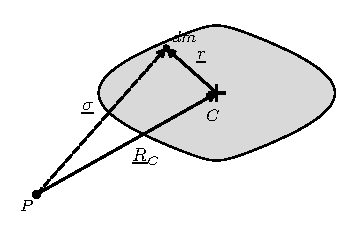
\includegraphics[width=0.36\linewidth]{parallel_axis}\end{center}

\paragraph{Statement.} If the inertia dyad about the centre of mass $\underrightarrow I_C$ is known, the dyad about any point $P$ is
\begin{equation}
\boxed{\;\underrightarrow{I}_{P}=\underrightarrow{I}_{C}+M\left(R_{C}^{2}\,\underrightarrow{1}-\underline{R}_{C}\,\underline{R}_{C}^T\right)\;}
\end{equation}
i.e.\ the inertia about $P$ equals the inertia about $C$ plus the inertia of a point mass $M$ placed at $C$.

\paragraph{Proof.} Substituting $\underline\sigma=\underline R_C+\underline r$:
\begin{equation}
\begin{aligned}
\underrightarrow{I}_{P}&=\int_{\mathcal{B}}\left[\left(\underline{R}_{C}+\underline{r}\right)\cdot\left(\underline{R}_{C}+\underline{r}\right)\underrightarrow{1}-\left(\underline{R}_{C}+\underline{r}\right)\left(\underline{R}_{C}+\underline{r}\right)^T\right]dm\\
&=MR_{C}^{2}\,\underrightarrow{1}+2\,\underline{R}_{C}\cdot\left(\int_{\mathcal{B}}\underline{r}\,dm\right)\underrightarrow{1}+\int_{\mathcal{B}}r^{2}\,\underrightarrow{1}\,dm
-M\underline{R}_{C}\underline{R}_{C}^T\\
&\quad-\int_{\mathcal{B}}\underline{r}\,\underline{r}^T dm
-\underline{R}_{C}\int_{\mathcal{B}}\underline{r}^T dm-\int_{\mathcal{B}}\underline{r}\,dm\,\underline{R}_{C}^T .
\end{aligned}
\end{equation}
$\underline R_C$ is the same for all $dm$ and can be taken out of the integrals. Since $\underline r$ is measured from the centre of mass,
$\int_{\mathcal B}\underline r\,dm=\underline 0$: the three mixed terms vanish. What remains is
\begin{equation}
\underrightarrow{I}_{P}=M\left(R_{C}^{2}\,\underrightarrow{1}-\underline{R}_{C}\underline{R}_{C}^T\right)+\int_{\mathcal{B}}\left(r^{2}\,\underrightarrow{1}-\underline{r}\,\underline{r}^T\right)dm
=\underrightarrow{I}_{C}+M\left(R_{C}^{2}\,\underrightarrow{1}-\underline{R}_{C}\underline{R}_{C}^T\right).\qquad\blacksquare
\end{equation}

\paragraph{Matrix form.} Projecting on body axes $(\hat b_1,\hat b_2,\hat b_3)$ (pre- and post-multiplying by the basis), with
$\underline R_C=x_C\hat b_1+y_C\hat b_2+z_C\hat b_3$:
\begin{equation}
\underline{\underline{I}}_P^{(B)}=\underline{\underline{I}}_{C}^{(B)}+M\begin{bmatrix}y_{C}^{2}+z_{C}^{2}&-x_{C}y_{C}&-x_{C}z_{C}\\-y_{C}x_{C}&x_{C}^{2}+z_{C}^{2}&-y_{C}z_{C}\\-z_{C}x_{C}&-z_{C}y_{C}&x_{C}^{2}+y_{C}^{2}\end{bmatrix}.
\end{equation}
For a single axis $\hat a$ through $P$ (parallel to an axis through $C$ at distance $d$): $I_{P,\hat a}=\hat a\cdot\underrightarrow I_P\cdot\hat a=I_{C,\hat a}+Md^2$,
since $R_C^2-(\hat a\cdot\underline R_C)^2=d^2$ (classical Huygens--Steiner form).

\paragraph{Remarks.} The theorem holds only between the centre of mass and another point (not between two generic points); moments of
inertia are minimum about axes through $C$; it is used to compute the inertia of a spacecraft from its components (bus, panels, booms).

\begin{keyf}
$\underrightarrow I_P=\int(\sigma^2\underrightarrow1-\underline\sigma\underline\sigma^T)dm$, \ $\underline\sigma=\underline R_C+\underline r$, \ $\int\underline r\,dm=\underline 0$ $\Rightarrow$
$\underrightarrow I_P=\underrightarrow I_C+M(R_C^2\underrightarrow1-\underline R_C\underline R_C^T)$; \ $I_{P,\hat a}=I_{C,\hat a}+Md^2$.
\end{keyf}

\pitfalls
\begin{itemize}
\item Say explicitly that the mixed terms vanish \emph{because $C$ is the centre of mass}.
\item Products of inertia also change: $-Mx_Cy_C$ etc.\ (with the minus sign, consistent with the definition of $\underline{\underline I}$).
\end{itemize}

\source{cap11.tex l.60--176 (inertia dyad and matrix), l.289--327 (parallel axis theorem, dyadic and matrix form). Formulario: \fml{11-PAT}.}

% ---------------------------------------------------------------------
\question{D7}{Inertia dyad, inertia matrix and its expression in two frames}
% source: cap11.tex l.32-58 (H), l.60-176 (dyad), l.178-227 (properties), l.229-287 (frames, principal axes)
\begin{qbox}
Define the inertia dyad (no derivation) and relate it to the inertia matrix. Derive the rotation matrix that expresses the inertia
matrix in two reference frames.
\qmeta{$\times$2 in the list (2025); Jan 2025; Sep 2024 (only: define the inertia dyad and relate it to the inertia matrix).}
\qnote{If only the first part is asked (Sep 2024): write points 1--2 of the outline and the properties.}
\end{qbox}

\begin{outline}
\begin{enumerate}
\item Angular momentum about $C$: $\underline H_C=\int\underline r\times(\underline\omega\times\underline r)dm=\underrightarrow I_C\cdot\underline\omega$; dyad $\underrightarrow I_C=\int(r^2\underrightarrow1-\underline r\,\underline r)dm$.
\item Inertia matrix = components of the dyad in a basis: $\underrightarrow I_C=[\hat b]\,\underline{\underline I}_C^{(B)}\,[\hat b]^T$; explicit matrix; $\underline H^{(B)}=\underline{\underline I}^{(B)}\underline\omega^{(B)}$.
\item Change of frame: $[\hat b]^T=\underline{\underline R}_{B\leftarrow A}[\hat a]^T$ $\Rightarrow$ $\underline{\underline I}_C^{(A)}=\underline{\underline R}_{B\leftarrow A}^T\underline{\underline I}_C^{(B)}\underline{\underline R}_{B\leftarrow A}$ (similar matrices).
\item Properties: symmetric, positive (semi)definite, triangular inequalities; principal axes diagonalise it.
\end{enumerate}
\end{outline}

\answer
\paragraph{Inertia dyad.} For a rigid body with centre of mass $C$, $\underline r$ = position of $dm$ from $C$ (fixed in the body frame, so
$\dot{\underline r}=\underline\omega\times\underline r$), the angular momentum about $C$ is
\begin{equation}
\underline H_C=\int_{\mathcal B}\underline r\times(\underline\omega\times\underline r)\,dm=\left(\int_{\mathcal B}\left[r^2\underrightarrow{1}-\underline r\,\underline r^T\right]dm\right)\cdot\underline\omega
=\underrightarrow{I}_C\cdot\underline\omega,
\end{equation}
\begin{equation}
\boxed{\;\underrightarrow{I}_C=\int_{\mathcal B}\left[r^2\,\underrightarrow{1}-\underline r\,\underline r^T\right]dm\;}\qquad
\underrightarrow1=\hat b_1\hat b_1+\hat b_2\hat b_2+\hat b_3\hat b_3 .
\end{equation}
The inertia dyad is a second-order tensor, independent of any frame, that depends only on the mass distribution; acting on
$\underline\omega$ it gives $\underline H_C$.

\paragraph{Relation with the inertia matrix.} Writing $\underline r=x\hat b_1+y\hat b_2+z\hat b_3$ in a frame $B$:
\begin{equation}
\underrightarrow{I}_C=[\hat b_1\ \hat b_2\ \hat b_3]\;\underline{\underline I}_C^{(B)}\;[\hat b_1\ \hat b_2\ \hat b_3]^T,\qquad
\underline{\underline{I}}_{C}^{(B)}=\int_{\mathcal{B}}\begin{bmatrix}y^{2}+z^{2}&-xy&-xz\\-yx&x^{2}+z^{2}&-yz\\-zx&-zy&x^{2}+y^{2}\end{bmatrix}dm .
\end{equation}
The \textbf{inertia matrix} is the projection (matrix of components) of the dyad on the basis $B$:
$\underline{\underline I}_C^{(B)}=[\hat b]^T\cdot\underrightarrow I_C\cdot[\hat b]$, since $[\hat b]^T\cdot[\hat b]=\underline{\underline I}_{3\times3}$. Diagonal terms: moments
of inertia; off-diagonal terms: products of inertia. In components, $\underline H_C^{(B)}=\underline{\underline I}_C^{(B)}\underline\omega^{(B)}$. The
same dyad has different matrices in different frames.

\paragraph{Inertia matrix in two frames (derivation).} Let $\underline{\underline I}_C^{(B)}$ be known and $A$ another frame, with
\begin{equation}
\begin{bmatrix}\hat b_1\\ \hat b_2\\ \hat b_3\end{bmatrix}=\underset{B\leftarrow A}{\underline{\underline{R}}}\begin{bmatrix}\hat a_1\\ \hat a_2\\ \hat a_3\end{bmatrix}
\iff [\hat b_1\ \hat b_2\ \hat b_3]=[\hat a_1\ \hat a_2\ \hat a_3]\,\underset{B\leftarrow A}{\underline{\underline{R}}}^{T}.
\end{equation}
Inserting in the expression of the dyad:
\begin{equation}
\underrightarrow{I}_C=[\hat b]\,\underline{\underline I}_C^{(B)}[\hat b]^T
=[\hat a_1\ \hat a_2\ \hat a_3]\;\underbrace{\underset{B\leftarrow A}{\underline{\underline{R}}}^{T}\underline{\underline I}_C^{(B)}\underset{B\leftarrow A}{\underline{\underline{R}}}}_{\underline{\underline I}_C^{(A)}}\;
\begin{bmatrix}\hat a_1\\ \hat a_2\\ \hat a_3\end{bmatrix},
\end{equation}
and since the dyad is unique, the matrix in brackets is its component matrix in $A$:
\begin{equation}
\boxed{\;\underline{\underline{I}}_{C}^{(A)}=\underset{B\leftarrow A}{\underline{\underline{R}}}^{T}\,\underline{\underline{I}}_{C}^{(B)}\,\underset{B\leftarrow A}{\underline{\underline{R}}}
=\underset{A\leftarrow B}{\underline{\underline{R}}}\,\underline{\underline{I}}_{C}^{(B)}\,\underset{B\leftarrow A}{\underline{\underline{R}}}\;}
\end{equation}
The two matrices are \textbf{similar} ($\underline{\underline R}^T=\underline{\underline R}^{-1}$): same eigenvalues (principal moments), same trace and
determinant. Check: $\underline H^{(A)}=\underline{\underline R}^T\underline H^{(B)}=\underline{\underline R}^T\underline{\underline I}^{(B)}\underline{\underline R}\,\underline\omega^{(A)}$.

\paragraph{Properties and principal axes.}
\begin{itemize}
\item \textbf{Symmetric}: real eigenvalues and real, orthogonal eigenvectors.
\item \textbf{Triangular inequalities}: $I_{11}\le I_{22}+I_{33}$ (and cyclic).
\item \textbf{Positive (semi)definite}: $\underline v^T\underline{\underline I}\underline v=\int v^2r^2(1-\cos^2\phi)dm\ge0$.
\item With $\underline{\underline T}$ = matrix of the eigenvectors ($\det\underline{\underline T}=1$, a rotation matrix), the similarity transformation gives a diagonal matrix:
$\underline{\underline I}_C^{(E)}=\underline{\underline T}^{-1}\underline{\underline I}_C^{(B)}\underline{\underline T}=\mathrm{diag}(\lambda_1,\lambda_2,\lambda_3)$: the eigenvectors are the
\textbf{principal axes of inertia}, $\underset{E\leftarrow B}{\underline{\underline R}}=\underline{\underline T}^T$.
\end{itemize}

\begin{keyf}
$\underrightarrow I_C=\int(r^2\underrightarrow1-\underline r\underline r^T)dm$, \ $\underline H_C=\underrightarrow I_C\cdot\underline\omega$, \ $\underrightarrow I_C=[\hat b]\underline{\underline I}^{(B)}[\hat b]^T$, \
$\underline{\underline I}^{(A)}=\underline{\underline R}_{B\leftarrow A}^T\underline{\underline I}^{(B)}\underline{\underline R}_{B\leftarrow A}$.
\end{keyf}

\pitfalls
\begin{itemize}
\item Distinguish the dyad (frame-independent tensor) from the matrix (its components in a basis).
\item Order of the product: with $[\hat b]^T=\underline{\underline R}_{B\leftarrow A}[\hat a]^T$, it is $\underline{\underline R}^T\underline{\underline I}^{(B)}\underline{\underline R}$, not $\underline{\underline R}\,\underline{\underline I}^{(B)}\underline{\underline R}^T$.
\item Off-diagonal elements have a minus sign ($-\int xy\,dm$).
\end{itemize}

\source{cap11.tex l.32--58 (angular momentum), l.60--176 (inertia dyad and matrix), l.178--227 (properties), l.229--274 (different
frames), l.276--287 (principal axes). Formulario: \fml{11-HIN}, \fml{11-IRF}.}

% ---------------------------------------------------------------------
\question{D8}{Torque-free equilibria and their stability without energy dissipation}
% source: cap11.tex l.386-446 (Euler eqs), l.709-751 (equilibria), l.753-816 (stability), l.818-905 (integrals)
\begin{qbox}
List the equilibrium conditions for torque-free attitude motion and comment on their stability in the absence of internal energy
dissipation. Sketch the intersection of the angular-momentum sphere with the energy ellipsoid.
\qmeta{$\times$2 in the list (2025); Feb 2025.}
\qnote{Difference from \qref{D9}: no dissipation (rigid body, $T_{rot}$ constant).}
\end{qbox}

\begin{outline}
\begin{enumerate}
\item Euler's equations in principal axes with $\underline L=\underline 0$.
\item Equilibrium: $\underline\omega$ fixed in the body; cases (a) $\omega=0$, (b) spherical: any axis, (c) axisymmetric: symmetry axis or any transverse axis, (d) general: pure spin about a principal axis.
\item Linear stability of pure spin: $\lambda=\pm\omega_{30}\sqrt{(I_2-I_3)(I_3-I_1)/(I_1I_2)}$: max/min axis imaginary, intermediate axis real $\Rightarrow$ unstable.
\item Integrals: momentum sphere $\sum H_i^2=H^2$, energy ellipsoid $\sum H_i^2/I_i=2T$; polhodes = intersections; $H^2/2I_1\le T\le H^2/2I_3$.
\item Sketch: closed curves around max and min axes (neutrally stable), separatrices through the intermediate axis (unstable).
\end{enumerate}
\end{outline}

\answer
\paragraph{Euler's equations without torque.} In principal axes ($\underline{\underline I}=\mathrm{diag}(I_1,I_2,I_3)$) and with $\underline L=\underline 0$:
\begin{equation}
I_{1}\dot{\omega}_{1}=\left(I_{2}-I_{3}\right)\omega_{2}\omega_{3},\qquad
I_{2}\dot{\omega}_{2}=\left(I_{3}-I_{1}\right)\omega_{1}\omega_{3},\qquad
I_{3}\dot{\omega}_{3}=\left(I_{1}-I_{2}\right)\omega_{1}\omega_{2}.
\end{equation}

\paragraph{Equilibrium solutions.} Look for motions with $\underline\omega$ aligned with a direction $\hat a$ fixed in the body,
$\underline\omega=\omega(t)[a_1\ a_2\ a_3][\hat e_1\ \hat e_2\ \hat e_3]^T$. Substituting:
$\dot\omega=\frac{I_2-I_3}{I_1}\frac{a_2a_3}{a_1}\omega^2=\frac{I_3-I_1}{I_2}\frac{a_1a_3}{a_2}\omega^2=\frac{I_1-I_2}{I_3}\frac{a_1a_2}{a_3}\omega^2$, i.e.
$\omega^{2}a_{2}^{2}a_{3}^{2}(I_{2}-I_{3})I_{2}I_{3}=\omega^{2}a_{1}^{2}a_{3}^{2}(I_{3}-I_{1})I_{1}I_{3}=\omega^{2}a_{1}^{2}a_{2}^{2}(I_{1}-I_{2})I_{1}I_{2}$. These hold if:
\begin{enumerate}[label=(\alph*)]
\item $\omega=0$: no rotation;
\item $I_1=I_2=I_3$ (spherical mass distribution): satisfied for any $(a_1,a_2,a_3)$: \textbf{rotation about any axis};
\item $I_1=I_2\neq I_3$ (axisymmetric about $\hat e_3$): $a_3=0$ or $a_1=a_2=0$: rotation \textbf{about the symmetry axis or about any axis perpendicular to it};
\item $I_1<I_2<I_3$ (general body): two components of $\hat a$ must vanish: \textbf{pure spin about one of the principal axes of inertia}.
\end{enumerate}
In general, pure spin about a principal axis of inertia is an equilibrium solution (then $\dot\omega=0$: constant angular velocity).

\paragraph{Linear stability of pure spin.} Perturb a spin about $\hat e_3$: $\omega_1=\delta\omega_1$, $\omega_2=\delta\omega_2$,
$\omega_3=\omega_{30}+\delta\omega_3$. To first order $\delta\dot\omega_3\simeq0$ and
\begin{equation}
\begin{bmatrix}\delta\dot\omega_1\\ \delta\dot\omega_2\end{bmatrix}=\omega_{30}\begin{bmatrix}0&\frac{I_2-I_3}{I_1}\\ \frac{I_3-I_1}{I_2}&0\end{bmatrix}\begin{bmatrix}\delta\omega_1\\ \delta\omega_2\end{bmatrix}
\ \Rightarrow\ \lambda_{1,2}=\pm\omega_{30}\sqrt{\frac{(I_2-I_3)(I_3-I_1)}{I_1I_2}} .
\end{equation}
If $I_3$ is the \textbf{maximum or minimum} moment, $(I_2-I_3)(I_3-I_1)<0$: imaginary eigenvalues, bounded oscillations (simply stable in
the linear sense). If $I_3$ is the \textbf{intermediate} one, one eigenvalue is real and positive: the perturbation grows exponentially
\textbf{(unstable)}. Linearisation is inconclusive for imaginary eigenvalues, so the conservation laws are used.

\paragraph{Momentum sphere and energy ellipsoid.} Without torques $\underline H_C$ is constant, and the rotational kinetic energy is constant too
($\dot T_{rot}=\underline\omega\cdot\underline L_C=0$ for a rigid body). With $H_i=I_i\omega_i$:
\begin{equation}
H_1^2+H_2^2+H_3^2=H^2\quad\text{(momentum sphere, radius $H$)},\qquad
\frac{H_1^2}{I_1}+\frac{H_2^2}{I_2}+\frac{H_3^2}{I_3}=2T_{rot}\quad\text{(energy ellipsoid)},
\end{equation}
the ellipsoid having semi-axes $a_i=\sqrt{2I_iT_{rot}}$. The motion must lie on both: the possible trajectories (polhodes) are their
\textbf{intersections}. For given $H$ only a range of energy is feasible (with $I_1>I_2>I_3$):
$T_{\min}=\frac{H^2}{2I_1}\le T_{rot}\le T_{\max}=\frac{H^2}{2I_3}$.
\begin{itemize}
\item $T=T_{\max}$: two intersection points $(0,0,\pm H)$: pure spin about the \textbf{minimum}-inertia axis $\hat e_3$;
\item $T=T_{\min}$: two points $(\pm H,0,0)$: pure spin about the \textbf{maximum}-inertia axis $\hat e_1$;
\item $T=H^2/2I_2$: two circles (the \textbf{separatrices}) crossing at $(0,\pm H,0)$: spin about the intermediate axis.
\end{itemize}
\begin{center}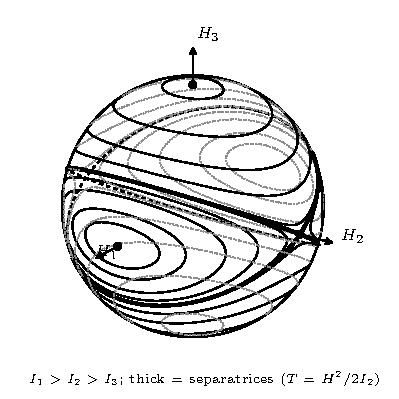
\includegraphics[width=0.48\linewidth]{polhodes}\hfill
\begin{minipage}[b]{0.46\linewidth}\small
Polhodes on the momentum sphere for $I_1:I_2:I_3=3:2:1$ (computed). Near $\hat e_1$ and $\hat e_3$ the curves are small closed loops:
a small perturbation keeps $\underline\omega$ close to the axis (\textbf{neutral stability}). Through $\hat e_2$ pass the separatrices (thick):
a small perturbation moves the state far away along them (\textbf{instability}).
\end{minipage}
\end{center}

\paragraph{Result (no dissipation).}
\begin{center}
\small
\begin{tabular}{@{}lc@{}}
\toprule
spin about & stability, rigid body\\
\midrule
maximum-inertia axis & (neutrally) stable\\
intermediate-inertia axis & unstable\\
minimum-inertia axis & (neutrally) stable\\
\bottomrule
\end{tabular}
\end{center}

\begin{fig2draw}
A circle (sphere) with three axes $H_1$ (max $I$), $H_2$, $H_3$ (min $I$). Small closed ovals around the $H_1$ and $H_3$ points; two
great circles (X shape) crossing at the $H_2$ points; label $T_{\min}$, $T_{\max}$ and the separatrix $T=H^2/2I_2$.
\end{fig2draw}

\begin{keyf}
Equilibria: pure spin about a principal axis (any axis if spherical; symmetry or transverse axis if axisymmetric); \
$\lambda=\pm\omega_{30}\sqrt{\frac{(I_2-I_3)(I_3-I_1)}{I_1I_2}}$; \ $\sum H_i^2=H^2$, $\sum H_i^2/I_i=2T$; \ $H^2/2I_{\max}\le T\le H^2/2I_{\min}$.
\end{keyf}

\pitfalls
\begin{itemize}
\item Without dissipation \emph{both} the maximum and the minimum axis are (neutrally) stable; only the intermediate one is unstable.
\item Explain why linearisation is not conclusive and how the sphere/ellipsoid argument completes it.
\item With $I_1>I_2>I_3$: maximum energy $\leftrightarrow$ minimum-inertia axis.
\end{itemize}

\source{cap11.tex l.386--446 (Euler's equations), l.448--473 (kinetic energy), l.709--751 (equilibrium solutions; errata \#17),
l.753--816 (stability of pure spin), l.818--905 (energy and momentum integrals, polhodes). Formulario: \fml{11-EQS}, \fml{11-MAX}.}

% ---------------------------------------------------------------------
\question{D9}{Torque-free equilibria and their stability with internal energy dissipation}
% source: cap11.tex l.709-905 (equilibria, integrals, dissipation), l.909-977 (nutation of axisymmetric bodies)
\begin{qbox}
List the equilibrium conditions for torque-free attitude motion and comment on their stability in the presence of internal energy
dissipation. Define the momentum sphere and the energy ellipsoid. Provide a sketch of a curve that represents the intersection of the
momentum sphere and the energy ellipsoid while energy reduces.
\qmeta{Jun 2025 (listed as a 2025 question).}
\qnote{Difference from \qref{D8}: internal dissipation ($\dot T_{rot}<0$, $\underline H$ constant) changes the stability of the minimum axis.}
\end{qbox}

\begin{outline}
\begin{enumerate}
\item Euler's equations without torque; equilibria: pure spin about a principal axis (+ spherical, axisymmetric cases).
\item Momentum sphere $\sum H_i^2=H^2$ and energy ellipsoid $\sum H_i^2/I_i=2T_{rot}$ (definitions, semi-axes); polhodes.
\item Dissipation: internal $\Rightarrow$ $\underline H$ constant, $T_{rot}$ decreases towards $T_{\min}=H^2/2I_{\max}$.
\item Sketch: path spiralling away from the min axis, crossing the separatrix, converging to the max axis.
\item Table: max axis asymptotically stable, min and intermediate unstable; examples (Explorer 1, Earth); axisymmetric bodies (oblate/prolate).
\end{enumerate}
\end{outline}

\answer
\paragraph{Equilibria.} In principal axes and without external torque, $I_1\dot\omega_1=(I_2-I_3)\omega_2\omega_3$ and cyclic. Steady rotations
with $\underline\omega$ fixed in the body exist if: (a) $\omega=0$; (b) spherical body ($I_1=I_2=I_3$): about any axis; (c) axisymmetric
body ($I_1=I_2\neq I_3$): about the symmetry axis or any transverse axis; (d) general body: \textbf{pure spin about one of the principal axes}.
Linearising about a spin $\omega_{30}$: $\lambda=\pm\omega_{30}\sqrt{(I_2-I_3)(I_3-I_1)/(I_1I_2)}$: real (unstable) if the spin axis is the
intermediate one, imaginary if it is the maximum or minimum one (inconclusive): the energy and momentum integrals decide.

\paragraph{Momentum sphere and energy ellipsoid.} With components $H_i=I_i\omega_i$ along the principal axes:
\begin{itemize}
\item \textbf{momentum sphere}: $H_1^2+H_2^2+H_3^2=H^2$ -- locus of the states with the given angular momentum magnitude (sphere of radius $H$);
without external torque $\underline H_C$ is constant, so the state always lies on it;
\item \textbf{energy ellipsoid} (Poinsot): $\frac{H_1^2}{I_1}+\frac{H_2^2}{I_2}+\frac{H_3^2}{I_3}=2T_{rot}$, i.e.\
$\frac{H_1^2}{a_1^2}+\frac{H_2^2}{a_2^2}+\frac{H_3^2}{a_3^2}=1$ with $a_i=\sqrt{2I_iT_{rot}}$ (largest axis along the maximum-inertia axis).
\end{itemize}
The actual motion is on their intersection (polhode). For given $H$, $\frac{H^2}{2I_{\max}}\le T_{rot}\le\frac{H^2}{2I_{\min}}$: maximum energy
= spin about the minimum-inertia axis, minimum energy = spin about the maximum-inertia axis; the separatrices ($T=H^2/2I_{int}$) pass
through the intermediate axis.

\paragraph{Effect of internal energy dissipation.} A real spacecraft is not perfectly rigid: flexible parts, fuel sloshing, nutation dampers
dissipate energy. These are \emph{internal} effects: they produce no external torque, so \textbf{$\underline H$ (and $|\underline H|$) stays constant}
while \textbf{$T_{rot}$ decreases}. The state remains on the same momentum sphere but moves to ellipsoids of lower and lower energy: the
polhode is no longer closed but slowly drifts, \textbf{crossing the separatrix}, until $T_{rot}$ reaches its minimum $T_{\min}=H^2/2I_{\max}$,
which corresponds to pure spin about the \textbf{maximum-inertia axis}.
\begin{center}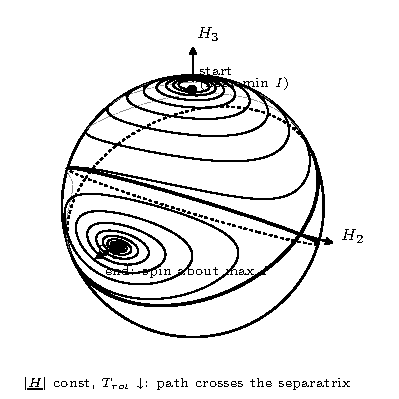
\includegraphics[width=0.48\linewidth]{polhodes_diss}\hfill
\begin{minipage}[b]{0.46\linewidth}\small
Path computed by integrating Euler's equations with a small dissipative term that keeps $|\underline H|$ constant and lowers $T_{rot}$
($I_1:I_2:I_3=3:2:1$). Starting near the minimum-inertia axis ($T\simeq T_{\max}$), the state spirals outwards (growing nutation),
crosses the separatrix (thick) and converges to the maximum-inertia axis: flat spin about $\hat e_1$.
\end{minipage}
\end{center}

\paragraph{Stability with dissipation.}
\begin{center}
\small
\begin{tabular}{@{}lcc@{}}
\toprule
spin about & no dissipation & with dissipation\\
\midrule
minimum-inertia axis & (neutrally) stable & \textbf{unstable}\\
intermediate-inertia axis & unstable & unstable\\
maximum-inertia axis & (neutrally) stable & \textbf{(asymptotically) stable}\\
\bottomrule
\end{tabular}
\end{center}
Pure spin about the maximal inertia axis is the \textbf{only stable configuration} when dissipation is considered (major-axis rule). This
explains why celestial bodies (like the Earth) rotate about their maximal inertia axis, and why \textbf{Explorer 1}, launched spinning about
its axis of least inertia (a prolate body with flexible antennas), began to tumble.

\paragraph{Axisymmetric bodies ($I_1=I_2=I_T$).} $2I_3T_{rot}-H^2=I_T(I_3-I_T)(\omega_1^2+\omega_2^2)$; with $H$ constant and $\dot T_{rot}<0$:
\begin{itemize}
\item \textbf{oblate} ($I_3>I_T$): $\omega_1^2+\omega_2^2\to0$, the nutation is damped and the body tends to pure spin about $\hat e_3$,
with $\omega_{3f}=H/I_3$;
\item \textbf{prolate} ($I_3<I_T$): $\omega_1^2+\omega_2^2$ grows to the maximum compatible with $H$: \textbf{flat spin} about a transverse axis,
$\sqrt{\omega_{1f}^2+\omega_{2f}^2}=H/I_T$ (nutation angle $\theta\to\pi/2$).
\end{itemize}
Hence spin-stabilised satellites must spin about the axis of maximum inertia (or use active control).

\begin{fig2draw}
Sphere with axes $H_1$ (max $I$), $H_2$, $H_3$ (min $I$); the X-shaped separatrices through $H_2$; a spiral starting as a tiny loop around
$H_3$, widening, crossing a separatrix and tightening around $H_1$. Arrow: "$T_{rot}\downarrow$, $|\underline H|$ const".
\end{fig2draw}

\begin{keyf}
$\sum H_i^2=H^2$ (sphere), $\sum\frac{H_i^2}{I_i}=2T_{rot}$ (ellipsoid, $a_i=\sqrt{2I_iT}$); dissipation: $|\underline H|$ const, $T\downarrow\to\frac{H^2}{2I_{\max}}$;
only spin about the max-inertia axis stable; $\omega_f=H/I_{\max}$.
\end{keyf}

\pitfalls
\begin{itemize}
\item Internal dissipation does not change $\underline H$ (no external torque): only $T_{rot}$ decreases.
\item The minimum-inertia axis is stable for a rigid body but \emph{unstable} with dissipation.
\item In the sketch the curve must cross the separatrix and end at the maximum-inertia axis (minimum energy).
\end{itemize}

\source{cap11.tex l.709--751 (equilibria), l.753--816 (stability), l.818--905 (sphere, ellipsoid, dissipation, table, Explorer 1),
l.909--977 (nutation of axisymmetric bodies). Formulario: \fml{11-MAX}.}

% =====================================================================
% Group E -- Possible further questions: topics marked T / T&N in the course program that have not been asked so far
% Same format, shorter answers.
% =====================================================================
\qgroup{E}{Possible further questions (T topics never asked so far)}

Topics marked T or T\&N in \texttt{Exam\_Course\_INFO.pdf} that do not appear in the collected exams. They are grouped by
exam slot: E1--E13 can be the "third" orbital question (chapters 2, 3, 4, 5, 6), E14 a Chapter 8 question, E15--E19 the
attitude question. Answers are shorter than in groups A--D but follow the same structure.

\begin{center}
\small
\begin{tabular}{@{}llr@{\hspace{1.2em}}llr@{}}
\toprule
Q & Topic & Page & Q & Topic & Page\\
\midrule
\ref{q:E1} & Two-body problem, potential of a sphere & \pageref{q:E1} & \ref{q:E11} & Newton's law with propulsion & \pageref{q:E11}\\
\ref{q:E2} & Eccentricity vector & \pageref{q:E2} & \ref{q:E12} & Optimal staging & \pageref{q:E12}\\
\ref{q:E3} & Energy, vis-viva, cosmic velocities & \pageref{q:E3} & \ref{q:E13} & Ascent trajectory & \pageref{q:E13}\\
\ref{q:E4} & Kepler's equation & \pageref{q:E4} & \ref{q:E14} & Perturbations: overview & \pageref{q:E14}\\
\ref{q:E5} & Special trajectories & \pageref{q:E5} & \ref{q:E15} & Euler's principal rotation theorem & \pageref{q:E15}\\
\ref{q:E6} & ECI, LVLH, orbit elements & \pageref{q:E6} & \ref{q:E16} & Euler's equations, kinetic energy & \pageref{q:E16}\\
\ref{q:E7} & Ground track properties & \pageref{q:E7} & \ref{q:E17} & Inertia matrix: properties, symmetry & \pageref{q:E17}\\
\ref{q:E8} & Three-dimensional transfers & \pageref{q:E8} & \ref{q:E18} & Torque-free axisymmetric body & \pageref{q:E18}\\
\ref{q:E9} & Sphere of influence, flyby & \pageref{q:E9} & \ref{q:E19} & Manoeuvres of spinning satellites & \pageref{q:E19}\\
\ref{q:E10} & Problem of two bodies & \pageref{q:E10} & & & \\
\bottomrule
\end{tabular}
\end{center}

% ---------------------------------------------------------------------
\question{E1}{Two-body problem and potential of a spherical mass distribution}
% source: cap02.tex l.35-166
\begin{qbox}
State the fundamental principles of orbital mechanics, derive the equation of the restricted two-body problem and show that a
spherical mass distribution generates the same potential as a point mass.
\qmeta{never asked (Ch.\,2, T).}
\end{qbox}
\begin{outline}
\begin{enumerate}
\item Newton's 2nd law (inertial frame) and universal gravitation; equivalence principle.
\item Two-body problem: subtract the equations $\Rightarrow$ $\frac{d^2}{dt^2}(\underline R_2-\underline R_1)=-\frac{G(m_1+m_2)}{R_{12}^3}(\underline R_2-\underline R_1)$.
\item Restricted ($m_1\gg m_2$): $\ddot{\underline r}=-\frac{\mu}{r^3}\underline r$, $\mu=Gm_1$.
\item Potential $V=\mu/r$ ($\underline F=\nabla V$, $U=-V$); thin spherical shell $\Rightarrow$ same as a point mass at the centre; sum of shells.
\end{enumerate}
\end{outline}
\answer
\paragraph{Principles.} (A) Newton's 2nd law in an inertial frame, $\underline F=\frac{d}{dt}(m\underline v)$. (B) Universal gravitation:
$\underline F_1=G\frac{m_1m_2}{R_{12}^3}(\underline R_2-\underline R_1)=-\underline F_2$, $G=6.673\cdot10^{-11}$\,m$^3$kg$^{-1}$s$^{-2}$. The equivalence
principle allows identifying inertial and gravitational mass.

\paragraph{Two-body problem.} Writing $m_1\ddot{\underline R}_1=\underline F_1$, $m_2\ddot{\underline R}_2=\underline F_2$ and subtracting the accelerations:
\begin{equation}
\frac{d^{2}}{dt^{2}}\left(\underline{R}_{2}-\underline{R}_{1}\right)=-G\frac{m_{1}+m_{2}}{R_{12}^{3}}\left(\underline{R}_{2}-\underline{R}_{1}\right),
\end{equation}
the motion of body 2 relative to body 1. If $m_1\gg m_2$ (\textbf{restricted} two-body problem), $m_1+m_2\simeq m_1$ and the effect of 2 on
1 is negligible; with $\underline r=\underline R_2-\underline R_1$:
\begin{equation}
\frac{d^{2}\underline r}{dt^{2}}=-\frac{\mu}{r^{3}}\underline r,\qquad \mu=Gm_1\ (\mu_\oplus=398600.4\ \text{km}^3/\text{s}^2).
\end{equation}

\paragraph{Gravitational potential.} A conservative force derives from a potential $V$ ($\underline F=\nabla V$) or a potential energy $U=-V$
($\underline F=-\nabla U$). For a point mass, per unit mass, $V=\mu/r$, $U=-\mu/r$.

\paragraph{Spherical mass distribution.} A thin shell of radius $R$, uniform surface density $\sigma=m_1/(4\pi R^2)$; the ring at angle $\theta$
has $dm=2\pi R^2s_\theta d\theta\,\sigma$ at distance $\rho$ from the external point, $\rho^2=r^2+R^2-2rRc_\theta$. Then
$dV=Gm_2\,dm/\rho$ and, using $2\rho\,d\rho=2rRs_\theta d\theta$,
\begin{equation}
V=Gm_2\,2\pi R^2\sigma\int_{r-R}^{r+R}\frac{d\rho}{rR}=\frac{4\pi R^2\sigma\,Gm_2}{r}=G\frac{m_1m_2}{r}.
\end{equation}
A shell generates the same potential as a point mass at its centre; a spherical body is a sum of shells, so it does the same. This
justifies treating spherical planets as point masses (and is the starting point of the harmonic expansion when the body is not spherical).

\begin{keyf}
$\ddot{\underline r}=-\dfrac{\mu}{r^3}\underline r$, \ $\mu=G(m_1+m_2)\simeq Gm_1$, \ $V=\dfrac{\mu}{r}$, $U=-\dfrac{\mu}{r}$, \ shell: $V=G\dfrac{m_1m_2}{r}$ for $r>R$.
\end{keyf}
\pitfalls
\begin{itemize}
\item The relative motion uses $G(m_1+m_2)$; the restricted approximation replaces it with $Gm_1$.
\item The shell result holds for external points ($r>R$).
\end{itemize}
\source{cap02.tex l.35--95 (principles, two-body), l.96--166 (potential, spherical shells). Formulario: --.}

% ---------------------------------------------------------------------
\question{E2}{The eccentricity vector}
% source: cap02.tex l.203-251
\begin{qbox}
Prove that the eccentricity vector is a first integral of the restricted two-body problem and use it to obtain the polar equation of the orbit.
\qmeta{never asked (Ch.\,2, T).}
\end{qbox}
\begin{outline}
\begin{enumerate}
\item $\frac{d}{dt}(\underline h\times\underline v)=-\mu\,\frac{d\hat r}{dt}$.
\item $\underline e:=-\hat r+\frac{\underline v\times\underline h}{\mu}$ $\Rightarrow$ $\dot{\underline e}=\underline 0$.
\item $\underline h\cdot\underline e=0$: 5 independent integrals; $\underline e$ in the plane, towards periapsis.
\item $\underline r\cdot\underline e$ $\Rightarrow$ $r=\frac{h^2/\mu}{1+e\cos\theta_*}$.
\end{enumerate}
\end{outline}
\answer
\paragraph{Proof.} With $\underline h$ constant,
$\frac{d}{dt}(\underline h\times\underline v)=\underline h\times\dot{\underline v}=-\frac{\mu}{r^2}(\underline r\times\underline v)\times\hat r$.
With $(\underline a\times\underline b)\times\underline c=\underline b(\underline a\cdot\underline c)-\underline a(\underline b\cdot\underline c)$:
$(\underline r\times\underline v)\times\hat r=r\underline v-\dot r\,\underline r=r^2\frac{d\hat r}{dt}$ (since $\frac{d\hat r}{dt}=\frac{\underline v-\dot r\hat r}{r}$). Hence
\begin{equation}
\frac{d}{dt}\left(\underline h\times\underline v\right)=-\mu\frac{d\hat r}{dt}
\;\Longrightarrow\;
\underline{e}:=-\hat{r}+\frac{\underline{v}\times\underline{h}}{\mu},\qquad \frac{d\underline e}{dt}=-\frac{d\hat r}{dt}+\frac{d\hat r}{dt}=\underline 0 .
\end{equation}
(The notes reach the same result writing $\underline v=\dot r\hat r+\underline\omega\times\underline r$.)

\paragraph{Properties.} $\underline h\cdot\underline e=0$: $\underline e$ lies in the orbit plane and is inertially fixed. $\underline h$ and $\underline e$ give 5 (not 6)
independent scalar integrals. At periapsis ($\underline v\perp\underline r$), $\underline v\times\underline h=v_ph\,\hat r$, so $\underline e=(v_ph/\mu-1)\hat r_p$: $\underline e$
points towards the periapsis and $|\underline e|=e$ is the eccentricity.

\paragraph{Polar equation.} Let $\theta_*$ (true anomaly) be the angle from $\underline e$ to $\underline r$; for $h\neq0$:
\begin{equation}
\underline r\cdot\underline e=re\cos\theta_*=-r+\frac{\underline r\cdot(\underline v\times\underline h)}{\mu}=-r+\frac{h^2}{\mu}
\;\Longrightarrow\; r=\frac{p}{1+e\cos\theta_*},\quad p=\frac{h^2}{\mu},
\end{equation}
($\underline r\cdot(\underline v\times\underline h)=\underline h\cdot(\underline r\times\underline v)=h^2$): a conic with focus at the attracting body.
Also $\underline h\times\underline e$ gives the velocity $\underline v=\sqrt{\mu/p}\,(e\,\hat p+\hat\theta)$.
\begin{keyf}
$\underline e=-\hat r+\dfrac{\underline v\times\underline h}{\mu}$, \ $\dot{\underline e}=\underline 0$, \ $\underline e\cdot\underline h=0$, \ $r=\dfrac{h^2/\mu}{1+e\,c_{\theta_*}}$, \ $\underline v=\sqrt{\mu/p}\,(e\hat p+\hat\theta)$.
\end{keyf}
\pitfalls
\begin{itemize}
\item Sign convention: $-\hat r+\underline v\times\underline h/\mu$ (order $\underline v\times\underline h$).
\item Say why there are only 5 independent integrals.
\end{itemize}
\source{cap02.tex l.203--228 (eccentricity vector), l.230--251 (polar equation), l.372--410 (velocity). Formulario: \fml{2-HEV}, \fml{2-POL}.}

% ---------------------------------------------------------------------
\question{E3}{Specific energy, vis-viva equation and cosmic velocities}
% source: cap02.tex l.372-587, 929-945
\begin{qbox}
Define the specific energy of a Keplerian orbit, derive its expression in terms of the orbit elements, and define the cosmic velocities.
\qmeta{never asked (Ch.\,2, T\&N).}
\end{qbox}
\begin{outline}
\begin{enumerate}
\item Velocity components $v_r=\sqrt{\mu/p}\,e\,s_{\theta_*}$, $v_\theta=\sqrt{\mu/p}(1+ec_{\theta_*})$.
\item $\mathcal E=\frac{v^2}{2}-\frac{\mu}{r}=-\frac{\mu}{2p}(1-e^2)=-\frac{\mu}{2a}$; sign vs orbit type.
\item Vis-viva $a=(2/r-v^2/\mu)^{-1}$; $e=\sqrt{1-h^2/(\mu a)}$.
\item Cosmic velocities $v_I=\sqrt{\mu/r}$, $v_{II}=\sqrt{2\mu/r}$; $v_\infty$ for hyperbolas.
\end{enumerate}
\end{outline}
\answer
\paragraph{Energy.} $\mathcal E=\frac{v^2}{2}-\frac{\mu}{r}$ (kinetic + potential, per unit mass) is constant (gravity is conservative). With
$r=\frac{p}{1+ec_{\theta_*}}$ and $v^2=v_r^2+v_\theta^2=\frac{\mu}{p}(1+e^2+2ec_{\theta_*})$:
\begin{equation}
\mathcal E=\frac{\mu}{2p}\left(1+e^2+2ec_{\theta_*}\right)-\frac{\mu}{p}\left(1+ec_{\theta_*}\right)=-\frac{\mu}{2p}\left(1-e^2\right)=-\frac{\mu}{2a}.
\end{equation}
$\mathcal E<0$ ellipse ($|PE|>KE$), $=0$ parabola, $>0$ hyperbola ($|PE|<KE$); it depends only on $a$.

\paragraph{Vis-viva.} From $\frac{v^2}{2}-\frac{\mu}{r}=-\frac{\mu}{2a}$: $v^2=\mu\left(\frac2r-\frac1a\right)$, $a=\frac{\mu}{2\mu/r-v^2}$; with
$h=|\underline r\times\underline v|=\sqrt{\mu a(1-e^2)}$: $e=\sqrt{1-h^2/(\mu a)}$. Hence $r$ and $v$ at one point fix $a$ (size, energy) and $e$ (shape).
Special values: ellipse $v_{p,A}=\sqrt{\frac{\mu}{a}\frac{1\pm e}{1\mp e}}$; hyperbola $v_\infty=\sqrt{-\mu/a}=\sqrt{2\mathcal E}$ (hyperbolic excess
velocity); parabola $v=\sqrt{2\mu/r}\to0$.

\paragraph{Cosmic velocities} at a point at distance $r$:
\begin{itemize}
\item \textbf{first}, $v_I=\sqrt{\mu/r}$: horizontal velocity giving a circular orbit of radius $r$ ($\mathcal E=-\mu/2r$);
\item \textbf{second} (escape), $v_{II}=\sqrt{2\mu/r}=\sqrt2\,v_I$: gives $\mathcal E=0$, a parabola with periapsis $r$: escape with zero velocity at infinity.
\end{itemize}
At the Earth's surface $v_I\simeq7.9$\,km/s, $v_{II}\simeq11.2$\,km/s \notinnotes. See \qref{A3} for the full family of trajectories.
\begin{keyf}
$\mathcal E=\dfrac{v^2}{2}-\dfrac{\mu}{r}=-\dfrac{\mu}{2a}$, \ $v^2=\mu\left(\dfrac2r-\dfrac1a\right)$, \ $v_I=\sqrt{\dfrac{\mu}{r}}$, $v_{II}=\sqrt{\dfrac{2\mu}{r}}$, \ $v_\infty=\sqrt{-\dfrac{\mu}{a}}$.
\end{keyf}
\pitfalls
\begin{itemize}
\item $\mathcal E$ does not depend on $e$: orbits with the same $a$ have the same energy and period.
\item $a<0$ for hyperbolas, so that $\mathcal E=-\mu/2a>0$.
\end{itemize}
\source{cap02.tex l.372--530 (velocity), l.532--552 (cosmic velocities), l.554--587 (energy), l.929--945 (vis-viva). Formulario: \fml{2-ENE}, \fml{2-VIS}, \fml{2-COS}.}

% ---------------------------------------------------------------------
\question{E4}{Position in time: eccentric anomaly and Kepler's equation}
% source: cap02.tex l.589-792
\begin{qbox}
Introduce the eccentric anomaly and derive Kepler's equation for elliptic orbits; explain how it is solved.
\qmeta{never asked (Ch.\,2, T\&N).}
\end{qbox}
\begin{outline}
\begin{enumerate}
\item $\dot\theta_*=h/r^2$: integrable only numerically $\Rightarrow$ alternative via $E$.
\item Definition of $E$ (auxiliary circle): $x=ac_E$, $y=bs_E$; $\tan\frac E2=\sqrt{\frac{1-e}{1+e}}\tan\frac{\theta_*}{2}$; $r=a(1-ec_E)$.
\item $\dot E(1-ec_E)=\sqrt{\mu/a^3}$ $\Rightarrow$ $M=E-es_E$, $M-M_0=n(t-t_0)$.
\item Newton's method; period $T=2\pi\sqrt{a^3/\mu}$ (3rd Kepler law).
\end{enumerate}
\end{outline}
\answer
\paragraph{Motivation.} $\dot\theta_*=\frac{h}{r^2}=\sqrt{\frac{\mu}{p^3}}(1+ec_{\theta_*})^2$ relates true anomaly and time but must be integrated
numerically; for ellipses a cheaper method uses the \textbf{eccentric anomaly} $E$.

\paragraph{Eccentric anomaly.} In a frame centred at the centre of the ellipse ($x$ along the apse line), the spacecraft is at
$x=ea+rc_{\theta_*}$, $y=rs_{\theta_*}$; $E$ is defined by $x=ac_E$, $y=bs_E=a\sqrt{1-e^2}\,s_E$ (projection on the auxiliary circle). Then
\begin{equation}
\tan\frac E2=\frac{s_E}{1+c_E}=\sqrt{\frac{1-e}{1+e}}\tan\frac{\theta_*}{2},\qquad r=a\left(1-e\,c_E\right).
\end{equation}

\paragraph{Kepler's equation.} Differentiating the two expressions of $r$: $\dot r=ae\dot Es_E$ and $\dot r=\sqrt{\mu/a^3}\,\frac{ae\,s_{\theta_*}}{\sqrt{1-e^2}}$;
with $rs_{\theta_*}=bs_E$ this gives $\dot E(1-ec_E)=\sqrt{\mu/a^3}$, which integrates (separation of variables) to
\begin{equation}
\left(E-e\,s_{E}\right)-\left(E_{0}-e\,s_{E_{0}}\right)=\sqrt{\frac{\mu}{a^{3}}}\,(t-t_{0})
\quad\Longleftrightarrow\quad M-M_0=n\,(t-t_0),\qquad M:=E-e\,s_E,\ n=\sqrt{\mu/a^3}.
\end{equation}
The \textbf{mean anomaly} $M$ grows linearly in time. Time from position: $\theta_*\to E\to M\to t$ (explicit). Position from time:
$t\to M\to E$ (transcendental, numerical) $\to\theta_*$. Circular orbits: $\theta_*=E=M$.

\paragraph{Newton's method.} $f(E)=E-es_E-M=0$, $E_{k+1}=E_k-\frac{f(E_k)}{1-ec_{E_k}}$, starting from $E_1=M$; converges in a few iterations.
After one period $\Delta E=2\pi=nT$: $T=2\pi\sqrt{a^3/\mu}$, i.e.\ $T^2/a^3=4\pi^2/\mu$ (3rd Kepler law). Analogous laws: Barker's equation for
parabolas, hyperbolic anomaly for hyperbolas.
\begin{keyf}
$\tan\frac E2=\sqrt{\frac{1-e}{1+e}}\tan\frac{\theta_*}2$, \ $r=a(1-ec_E)$, \ $M=E-es_E=M_0+\sqrt{\mu/a^3}(t-t_0)$, \ $E_{k+1}=E_k-\dfrac{E_k-es_{E_k}-M}{1-ec_{E_k}}$, \ $T=2\pi\sqrt{a^3/\mu}$.
\end{keyf}
\pitfalls
\begin{itemize}
\item Use the half-angle formula to keep $E$ and $\theta_*$ in the same half-plane.
\item $E$, $M$ in radians; count full revolutions separately.
\end{itemize}
\source{cap02.tex l.589--615 ($\dot\theta_*$), l.617--748 (eccentric anomaly, Kepler's equation, Newton's method, 3rd law). Formulario: \fml{2-E2T}, \fml{2-KEP}, \fml{2-NEW}.}

% ---------------------------------------------------------------------
\question{E5}{Special Keplerian trajectories}
% source: cap02.tex l.794-891
\begin{qbox}
Describe the special Keplerian trajectories: circular orbits (with the balance of accelerations), geosynchronous, ballistic and rectilinear trajectories.
\qmeta{never asked (Ch.\,2, T).}
\end{qbox}
\begin{outline}
\begin{enumerate}
\item Circular: $r$, $v$ constant; acceleration in the rotating frame; gravity balances the centrifugal term.
\item Geosynchronous: $T=T_{sid}$, $a=42164$\,km (see \qref{A4}).
\item Ballistic: elliptic arcs with periapsis inside the Earth (ICBM).
\item Rectilinear: $h=0$, $e=1$, $p=0$; elliptic, parabolic, hyperbolic types.
\end{enumerate}
\end{outline}
\answer
\paragraph{Circular orbits.} $r=p=R$ and $v=\sqrt{\mu/R}$ are constant. In general
$\ddot{\underline r}=\ddot r\hat r+2\underline\omega\times(\dot r\hat r)+\dot{\underline\omega}\times\underline r+\underline\omega\times(\underline\omega\times\underline r)$
(radial, Coriolis, Euler, centripetal terms). On a circular orbit $\dot r=\ddot r=0$ and $\underline\omega=\underline h/R^2$ is constant, so
\begin{equation}
\ddot r\,\hat r=\underline 0=-\frac{\mu}{r^2}\hat r-\underline\omega\times(\underline\omega\times\underline r):
\end{equation}
the gravitational acceleration and the centrifugal (fictitious) acceleration balance at all times; the rotating frame attached to the
vehicle has no radial acceleration ($\omega^2R=\mu/R^2\Rightarrow v=\sqrt{\mu/R}$).

\paragraph{Geosynchronous orbits.} Period equal to the sidereal day (86164\,s): $a=42164$\,km, any $e$, $i$ (\qref{A4}).

\paragraph{Ballistic trajectories.} Arcs of ellipses whose periapsis lies \emph{inside} the Earth (apoapsis outside): the trajectory intersects
the surface twice. Used by ballistic missiles (ICBM) and sub-orbital flights.

\paragraph{Rectilinear trajectories.} $\underline v\parallel\underline r$ $\Rightarrow$ $\underline h=\underline 0$, $e=|-\hat r|=1$, $p=0$, $r_p=0$: motion along a line through the
attracting body ($\theta_*=\pm\pi$), non-uniform. Three types by energy: $a>0$, $\mathcal E<0$ \emph{rectilinear ellipse} (segment, falls back);
$a\to\infty$, $\mathcal E=0$ \emph{rectilinear parabola} ($v\to0$ at infinity); $a<0$, $\mathcal E>0$ \emph{rectilinear hyperbola} ($v$ does not vanish).
Example: vertical launch with no horizontal velocity.
\begin{keyf}
Circular: $\mu/R^2=\omega^2R$, $v=\sqrt{\mu/R}$; \ ballistic: $r_p<R_E$; \ rectilinear: $h=0$, $e=1$, type set by $\mathcal E=-\mu/2a$.
\end{keyf}
\pitfalls
\begin{itemize}
\item In the rotating frame the centrifugal term is fictitious; in the inertial frame gravity provides the centripetal acceleration.
\end{itemize}
\source{cap02.tex l.794--848 (circular), l.850--868 (geosynchronous), l.870--879 (ballistic), l.881--891 (rectilinear). Formulario: \fml{2-VCI}, \fml{2-BAL}.}

% ---------------------------------------------------------------------
\question{E6}{ECI and LVLH frames; orbit elements}
% source: cap02.tex l.1007-1156
\begin{qbox}
Define the Earth-centred inertial frame and the rotating LVLH frame, and the six orbit elements, including the special cases where some are undefined.
\qmeta{never asked (Ch.\,2, T\&N).}
\end{qbox}
\begin{outline}
\begin{enumerate}
\item ECI: $\hat c_3$ Earth axis (North), $\hat c_1$ vernal axis = ecliptic $\cap$ equator, $\hat c_2$ completes; precession of equinoxes neglected.
\item Orbit plane: $\Omega\in[-\pi,\pi[$, $i\in[0,\pi]$; $\omega$ from the node; $\theta_t=\omega+\theta_*$.
\item LVLH $(\hat r,\hat\theta,\hat h)=\underline{\underline R}_3(\theta_t)\underline{\underline R}_1(i)\underline{\underline R}_3(\Omega)(\hat c)$.
\item Elements $(a,e,i,\Omega,\omega)$ + one anomaly; special cases (circular, equatorial).
\end{enumerate}
\end{outline}
\answer
\paragraph{ECI frame.} Centred at the Earth's centre. $\hat c_3$ = Earth's rotation axis (towards the North pole); $\hat c_1$ = \textbf{vernal axis},
intersection of the ecliptic plane (plane of the Earth's orbit, normal to the ecliptic pole $\hat p$) with the equatorial plane; $\hat c_2=\hat c_3\times\hat c_1$.
Strictly, $\hat c_3$ precesses around $\hat p$ (precession of the equinoxes, $\sim$25\,700 years), but for satellite motion the axes are inertial.

\paragraph{Angles.} The orbit plane is identified by $\Omega$ (right ascension of the ascending node, $[-\pi,\pi[$, from $\hat c_1$ to the node $N$
where the spacecraft crosses the equator from South to North) and $i$ (inclination, $[0,\pi]$; direct $<90^\circ$, retrograde $>90^\circ$).
The \textbf{argument of perigee} $\omega\in[-\pi,\pi[$ is measured counter-clockwise from the nodal line to the periapsis; the argument of latitude
is $\theta_t=\omega+\theta_*$. Since $\underline h$ and $\underline e$ are first integrals, $(\Omega,i,\omega)$ are constant for Keplerian orbits.

\paragraph{LVLH frame} $(\hat r,\hat\theta,\hat h)$: radial, horizontal (in-plane, along the motion), normal to the orbit; it rotates with the spacecraft
(non-inertial) and is obtained from ECI with three counter-clockwise rotations:
\begin{equation}
\begin{bmatrix}\hat r\\ \hat\theta\\ \hat h\end{bmatrix}=\underline{\underline R}_3(\theta_t)\,\underline{\underline R}_1(i)\,\underline{\underline R}_3(\Omega)\begin{bmatrix}\hat c_1\\ \hat c_2\\ \hat c_3\end{bmatrix}.
\end{equation}

\paragraph{Orbit elements.} $a$ (size, energy), $e$ (shape), $(\Omega,i)$ (orientation of the plane), $\omega$ (periapsis in the plane): five constants
(five independent components of $\underline h$, $\underline e$); the sixth, time-varying, is one anomaly ($\theta_*$, $E$ or $M$), equivalent to the time of
periapsis passage. Special cases:
\begin{itemize}
\item circular ($e=0$): no periapsis, only $\theta_t$ is defined;
\item equatorial ($i=0,\pi$): no node, only the longitude of periapsis $\tilde\omega=\Omega\pm\omega$;
\item circular equatorial: only the true longitude $\tilde\lambda=\theta_t+\Omega$ ($i=0$) or $\Omega-\theta_t$ ($i=\pi$).
\end{itemize}
\begin{keyf}
$(\hat r,\hat\theta,\hat h)^T=\underline{\underline R}_3(\theta_t)\underline{\underline R}_1(i)\underline{\underline R}_3(\Omega)(\hat c_1,\hat c_2,\hat c_3)^T$, \ $\theta_t=\omega+\theta_*$; \
elements $(a,e,i,\Omega,\omega,\theta_*)$; $i\in[0,\pi]$, $\Omega,\omega\in[-\pi,\pi[$.
\end{keyf}
\pitfalls
\begin{itemize}
\item The ascending node is the South$\to$North crossing; $\omega$ is measured in the orbit plane from the node.
\end{itemize}
\source{cap02.tex l.1007--1099 (frames), l.1101--1156 (orbit elements). Formulario: \fml{2-OEL}, \fml{2-RA}.}

% ---------------------------------------------------------------------
\question{E7}{Ground track: latitude limits, symmetries, motion along the track}
% source: cap02.tex l.1657-1855
\begin{qbox}
Define the ground track and discuss its latitude limits, symmetry properties and the direction of motion along it.
\qmeta{never asked as a whole (Ch.\,2, T\&N); geosynchronous tracks in \qref{A4}.}
\end{qbox}
\begin{outline}
\begin{enumerate}
\item Definition; $\phi$ and $\lambda_g=\xi-\theta_g$ from the orbit elements.
\item Latitude limits: $\phi_{\max}=i$ (direct) or $\pi-i$ (retrograde); polar orbits.
\item Symmetries: $\omega=\pm\pi/2$ (meridian), $\omega=0,\pi$ (equator crossings), $e=0$ both.
\item Motion: retrograde always westward; direct depends on $a$, $e$, $\omega$; drift east if $T<T_{sid}$, west if $T>T_{sid}$.
\end{enumerate}
\end{outline}
\answer
\paragraph{Definition.} The ground track is the locus of the sub-satellite points on the rotating Earth, on a Mercator map ($\lambda_g$, $\phi$).
Equating the position written with orbit elements and with absolute longitude $\xi$ and latitude $\phi$:
\begin{equation}
s_\phi=s_{\theta_t}s_i,\qquad c_\xi=\frac{c_{\theta_t}c_\Omega-c_is_{\theta_t}s_\Omega}{c_\phi},\ \ s_\xi=\frac{c_{\theta_t}s_\Omega+c_is_{\theta_t}c_\Omega}{c_\phi},\qquad
\lambda_g=\xi-\theta_g,\ \ \theta_g=\theta_{g0}+\omega_E(t-t_0).
\end{equation}
\paragraph{Latitude limits.} $\phi=\arcsin(s_{\theta_t}s_i)$: extremes at $\theta_t=\pm\pi/2$. Direct orbits: $-i\le\phi\le i$; retrograde: $|\phi|\le\pi-i$
(latitude is in $[-\pi/2,\pi/2]$, inclination in $[0,\pi]$). Polar orbits ($i=\pi/2$) fly over all latitudes; crossing a pole the longitude jumps by
$\pi$ (Mercator discontinuity).
\paragraph{Symmetries} (from the symmetry of $\underline v$ w.r.t.\ the apsidal line and because points at the same latitude have the same eastward
inertial velocity): (a) $e\neq0$, $\omega=\pm\pi/2$: symmetric w.r.t.\ the meridian through the maximum/minimum latitude (apoapsis/periapsis);
(b) $e\neq0$, $\omega=0,\pi$: symmetric w.r.t.\ the equator-crossing points; (c) $e=0$: both. They allow reading $e$ and $\omega$ from a track.
\paragraph{Motion along the track.} \emph{Retrograde} orbits: the inertial velocity has a westward component, the track is always travelled East$\to$West.
\emph{Direct} orbits: the sub-satellite eastward velocity must be compared with that of the Earth at the same latitude: the track can be travelled
either way, depending on $a$, $e$, $\omega$. After one period the track point $P_1$ (same latitude and slope as $P_0$) moves east if
$T<T_{sid}$ (low orbits drift eastward) and west if $T>T_{sid}$ (high orbits move globally westward); geosynchronous direct orbits have closed
tracks, travelled partly westward and partly eastward.
\begin{keyf}
$s_\phi=s_{\theta_t}s_i$, $\lambda_g=\xi-\theta_g$; \ $\phi_{\max}=i$ (direct), $\pi-i$ (retrograde); \ drift east if $T<T_{sid}$, west if $T>T_{sid}$.
\end{keyf}
\pitfalls
\begin{itemize}
\item Retrograde: $\phi_{\max}=\pi-i$, not $i$.
\end{itemize}
\source{cap02.tex l.1657--1739 (ground track), l.1741--1796 (latitude, symmetry), l.1845--1855 (motion along the track). Formulario: \fml{2-LAT}, \fml{2-GTS}, \fml{2-GTD}.}

% ---------------------------------------------------------------------
\question{E8}{Three-dimensional orbit transfers}
% source: cap03.tex l.451-565
\begin{qbox}
Discuss in-plane and out-of-plane velocity changes in three-dimensional orbit transfers and describe a near-optimal LEO--GEO transfer.
\qmeta{never asked (Ch.\,3, T; LEO--GEO is N).}
\end{qbox}
\begin{outline}
\begin{enumerate}
\item In-plane: $dv=\frac{\mu}{2a^2v}da$ $\Rightarrow$ most efficient at periapsis (max $v$).
\item Out-of-plane: rotation by $\Delta\phi$ about $BP$, $|\Delta\underline v|=2v\,s_{\Delta\phi/2}$ $\Rightarrow$ at apoapsis (min $v$), at a node.
\item LEO--GEO: (A) 3 impulses; (B) 2 impulses combining circularisation and plane change; true optimum splits the plane change.
\item Reversibility of optimal transfers.
\end{enumerate}
\end{outline}
\answer
\paragraph{In-plane velocity changes.} From $\mathcal E=-\frac{\mu}{2a}=\frac{v^2}{2}-\frac{\mu}{r}$ at fixed $r$: $\frac{\mu}{2a^2}da=v\,dv$, i.e.\
$dv=\frac{\mu}{2a^2v}da$: the $\Delta v$ needed for a given change of $a$ is minimum where $v$ is maximum, at \textbf{periapsis}.
\paragraph{Out-of-plane velocity changes.} To rotate the orbit plane by $\Delta\phi$ about the line $BP$ ($B$ = attracting body) keeping the speed:
$|\underline v_0|=|\underline v_f|=v$ and
\begin{equation}
|\Delta\underline v|=2v\sin\frac{\Delta\phi}{2},
\end{equation}
expensive (e.g.\ $\Delta\phi=60^\circ$ costs $\Delta v=v$), so it is convenient where $v$ is minimum, at \textbf{apoapsis}; to change $i$ without changing
$\Omega$ the impulse must be at a node.
\paragraph{Near-optimal LEO--GEO transfer.} From a circular LEO ($R_i$, $i_0>0$) to a circular GEO ($R_f$, $i_f<i_0$):
(A) \emph{3 impulses}: at perigee raise $r_A$ to $R_f$; at apoapsis circularise; at a node rotate the plane by $i_0-i_f$.
(B) \emph{2 impulses}: first impulse at a node to raise $r_A=R_f$, second at the opposite node (the apoapsis) combining circularisation and
plane change: $\Delta v_2^{(B)}=\sqrt{v_A^2+v_{cf}^2-2v_Av_{cf}c_{\Delta\phi}}<\Delta v_2^{(A)}+\Delta v_3^{(A)}$, with
$v_A=\sqrt{\frac{2\mu}{R_i+R_f}\frac{R_i}{R_f}}$, $v_{cf}=\sqrt{\mu/R_f}$ (vector addition is cheaper than two separate impulses).
(B) is near-optimal; the true optimum also performs a small part of the plane change at the first impulse
($\Delta v_1=\sqrt{v_{ci}^2+v_{PH}^2-2v_{ci}v_{PH}c_{(i_1-i_H)}}$).
\paragraph{Remark.} If the transfer A$\to$B is optimal, the return transfer B$\to$A, with impulses of equal magnitude and opposite direction, is optimal
too (e.g.\ interior Hohmann transfer).
\begin{keyf}
$dv=\dfrac{\mu}{2a^2v}da$; \ $|\Delta v|=2v\sin\dfrac{\Delta\phi}{2}$; \ combined: $\Delta v=\sqrt{v_1^2+v_2^2-2v_1v_2\cos\Delta\phi}$.
\end{keyf}
\pitfalls
\begin{itemize}
\item In-plane at periapsis, plane changes at apoapsis (and at a node).
\end{itemize}
\source{cap03.tex l.451--537 (3D transfers, LEO--GEO), l.539--565 (concluding remarks). Formulario: \fml{3-3DV}, \fml{3-LGE}.}

% ---------------------------------------------------------------------
\question{E9}{Sphere of influence and qualitative effect of a flyby}
% source: cap04.tex l.20-126, l.522-600
\begin{qbox}
Introduce the patched-conic approximation and derive the radius of the sphere of influence; describe qualitatively the effect of a planetary flyby.
\qmeta{never asked (Ch.\,4: introduction T, SoI T\&N, qualitative flyby T).}
\end{qbox}
\begin{outline}
\begin{enumerate}
\item Patched conics: one attracting body at a time; departure hyperbola, heliocentric ellipse, arrival hyperbola.
\item Equations of the vehicle relative to the planet and to the Sun: dominant + perturbing terms.
\item SoI: equal ratios $\Rightarrow$ $\rho_{SoI}=L(m_p/m_s)^{2/5}$; values.
\item Flyby: $\underline v^{(H)}_\pm=\underline v^{(H)}_p+\underline v_\infty^\pm$; $|\underline v_\infty|$ unchanged, direction rotated $\Rightarrow$ heliocentric speed and energy change.
\item Behind the planet: increase; in front: decrease; clockwise/counter-clockwise.
\end{enumerate}
\end{outline}
\answer
\paragraph{Patched conics.} The spacecraft is assumed to be subject to \textbf{one attracting body at a time}: near the departure planet only its gravity
(hyperbola), far away only the Sun (heliocentric ellipse), near the arrival planet only its gravity (hyperbola). Each arc is Keplerian.

\paragraph{Sphere of influence.} For Sun ($S$), planet ($P$), vehicle ($V$), with $\underline\rho$ = vehicle w.r.t.\ planet, $\underline r$ = vehicle w.r.t.\ Sun,
$\underline L$ = planet w.r.t.\ Sun:
\begin{equation}
\ddot{\underline\rho}=-\frac{Gm_p}{\rho^3}\underline\rho-Gm_s\left[\frac{\underline r}{r^3}-\frac{\underline L}{L^3}\right],\qquad
\ddot{\underline r}=-\frac{Gm_s}{r^3}\underline r-Gm_p\frac{\underline\rho}{\rho^3}.
\end{equation}
In each equation the first term is the dominant attraction, the second the perturbation. The SoI is where the perturbation/dominant ratios are
equal:
$\frac{m_s|\underline r/r^3-\underline L/L^3|}{m_p/\rho^2}=\frac{m_p/\rho^2}{m_s/r^2}$. With $\frac{\underline r}{r^3}-\frac{\underline L}{L^3}\simeq\frac{\underline\rho}{L^3}$ and $r\simeq L$:
\begin{equation}
\left(\frac{\rho}{L}\right)^{5}=\left(\frac{m_p}{m_s}\right)^2\;\Longrightarrow\;\rho_{SoI}=L\left(\frac{m_p}{m_s}\right)^{2/5}.
\end{equation}
An estimate, not an exact boundary: Earth $9.24\cdot10^5$\,km, Mars $5.74\cdot10^5$\,km, Jupiter $4.83\cdot10^7$\,km, Neptune $8.67\cdot10^7$\,km (larger
than Jupiter's because it is farther from the Sun).

\paragraph{Flyby (qualitative).} Inside the SoI, with no manoeuvre, the spacecraft follows a hyperbola: the relative velocity at the SoI keeps its
magnitude $v_\infty$ but is rotated by the deflection angle. In the heliocentric frame
\begin{equation}
\underline v^{(H)}_\pm=\underline v_p^{(H)}+\underline v_\infty^\pm ,
\end{equation}
so the heliocentric velocity changes in magnitude and direction and the heliocentric energy changes ($\mathcal E_+\neq\mathcal E_-$). The energy is
exchanged with the planet, whose velocity change is negligible. Depending on the geometry a flyby can increase, leave unchanged or reduce the
heliocentric speed: \textbf{periapsis behind the planet} (passing behind it w.r.t.\ its motion) $\Rightarrow$ \textbf{increase}; hyperbola symmetric
w.r.t.\ $\underline v_p^{(H)}$ $\Rightarrow$ unchanged; \textbf{periapsis in front} $\Rightarrow$ \textbf{decrease}; this holds for both clockwise and counter-clockwise
flybys. Gravity assists made Voyager, Cassini, Ulysses (out of the ecliptic) feasible.
\begin{keyf}
$\rho_{SoI}=L\left(\dfrac{m_p}{m_s}\right)^{2/5}$; \ $\underline v^{(H)}_\pm=\underline v_p^{(H)}+\underline v_\infty^\pm$, $|\underline v_\infty^+|=|\underline v_\infty^-|$; \ behind $\Rightarrow$ speed up, in front $\Rightarrow$ slow down.
\end{keyf}
\pitfalls
\begin{itemize}
\item The speed relative to the planet does not change; the heliocentric one does.
\end{itemize}
\source{cap04.tex l.20--27 (patched conics), l.29--126 (sphere of influence), l.522--600 (flyby). Formulario: \fml{4-SOI}, \fml{4-FBC}.}

% ---------------------------------------------------------------------
\question{E10}{Problem of two bodies: relative and absolute motion}
% source: cap05.tex l.111-242
\begin{qbox}
Describe the motion of two bodies subject to their mutual attraction: relative motion, motion of the centre of mass and absolute motions.
\qmeta{never asked (Ch.\,5, T).}
\end{qbox}
\begin{outline}
\begin{enumerate}
\item Relative motion: Keplerian with $G(m_1+m_2)$.
\item Centre of mass on the line of the bodies, uniform motion; origin $O'$ there.
\item Absolute motions about $O'$: Keplerian with equivalent masses $m_2^3/M^2$, $m_1^3/M^2$.
\item Same eccentricity, $a_1/a_2=m_2/m_1$, $\omega^2=GM/(a_1+a_2)^3$; planet--satellite limit.
\end{enumerate}
\end{outline}
\answer
\paragraph{Relative motion.} From $m_1\ddot{\underline R}_1=\underline F_1$, $m_2\ddot{\underline R}_2=\underline F_2=-\underline F_1$:
$\frac{d^2}{dt^2}(\underline R_2-\underline R_1)=-\frac{G(m_1+m_2)}{r_{12}^3}(\underline R_2-\underline R_1)$: 2 moves relative to 1 as if the total mass
$M=m_1+m_2$ were at 1: Keplerian.
\paragraph{Centre of mass.} $\underline R_c=\frac{m_1\underline R_1+m_2\underline R_2}{M}$ lies on the segment joining the bodies
($\underline R_1-\underline R_c=\frac{m_2}{M}(\underline R_1-\underline R_2)$, opposite to $\underline R_2-\underline R_c$) and moves uniformly; take it as origin $O'$:
$m_1\underline R_1+m_2\underline R_2=\underline 0$, $m_1R_1=m_2R_2$.
\paragraph{Absolute motion.} With $r_{12}=R_1(1+m_1/m_2)$:
\begin{equation}
\ddot{\underline R}_1=-G\frac{m_2^3}{M^2}\frac{\underline R_1}{R_1^3},\qquad \ddot{\underline R}_2=-G\frac{m_1^3}{M^2}\frac{\underline R_2}{R_2^3}:
\end{equation}
each body moves on a Keplerian conic about $O'$ with equivalent mass $m_2^3/M^2$ (resp.\ $m_1^3/M^2$). Since $R_1/R_2=m_2/m_1$ is constant, the bodies
reach periapsis and apoapsis together: $\frac{a_1(1-e_1)}{a_2(1-e_2)}=\frac{a_1(1+e_1)}{a_2(1+e_2)}\Rightarrow e_1=e_2$, and $a_1/a_2=m_2/m_1$. The larger
mass moves entirely inside the orbit of the smaller one if $e<(m_1-m_2)/M$. Mean motion: $\omega^2=\frac{GM}{(a_1+a_2)^3}$.
\paragraph{Planet--satellite problem.} $m_1\gg m_2$: the centre of mass coincides with the planet's centre and the satellite obeys the classical
one-body equation (restricted two-body problem).
\begin{keyf}
Relative: $\mu=G(m_1+m_2)$; \ $m_1\underline R_1+m_2\underline R_2=\underline 0$; \ absolute: equivalent masses $m_2^3/M^2$, $m_1^3/M^2$; \ $e_1=e_2$, $\frac{a_1}{a_2}=\frac{m_2}{m_1}$, $\omega^2=\frac{GM}{(a_1+a_2)^3}$.
\end{keyf}
\pitfalls
\begin{itemize}
\item Relative and absolute motions are both Keplerian, but with different gravitational parameters.
\end{itemize}
\source{cap05.tex l.111--236 (problem of two bodies), l.238--242 (planet--satellite).}

% ---------------------------------------------------------------------
\question{E11}{Newton's law with propulsion: thrust and effective exhaust velocity}
% source: cap06.tex l.21-110
\begin{qbox}
Derive the equation of motion of a rocket (Newton's law with propulsion) and define thrust, effective exhaust velocity and specific impulse.
\qmeta{never asked (Ch.\,6, T).}
\end{qbox}
\begin{outline}
\begin{enumerate}
\item Momentum of vehicle + ejected mass at $t$ and $t+\Delta t$; external forces $\underline G+\underline A+\underline P_{ext}$, $\underline P_{ext}=(p_e-p_a)A_e\hat v$.
\item Limit $\Delta t\to0$: $m\dot{\underline v}+\dot{\tilde m}\underline c_{ej}=\underline G+\underline A+A_e(p_e-p_a)\hat v$.
\item $\underline T=\dot m\underline c$, $\underline c=\underline c_{ej}+A_e(p_e-p_a)\hat v/\dot m$, $\dot m=-T/c$; $\dot{\underline v}=(\underline G+\underline A+\underline T)/m$.
\item $c=g_0I_{sp}$.
\end{enumerate}
\end{outline}
\answer
\paragraph{Momentum balance.} At $t$ the vehicle has mass $m$ and velocity $\underline v$; after $\Delta t$ the ejected mass $\Delta\tilde m$ moves with
$\underline v+\underline c_{ej}$ ($\underline c_{ej}$ = exhaust velocity relative to the vehicle) and the vehicle has mass $m-\Delta\tilde m$ and velocity $\underline v+\Delta\underline v$:
\begin{equation}
\Delta\underline M=(m-\Delta\tilde m)(\underline v+\Delta\underline v)+\Delta\tilde m(\underline v+\underline c_{ej})-m\underline v .
\end{equation}
External forces: gravity $\underline G$, aerodynamic force $\underline A$ and the external pressure force; on the nozzle exit (area $A_e$, pressure $p_e$) vs
ambient pressure $p_a$, the net pressure force is $\underline P_{ext}=(p_e-p_a)A_e\hat v$. Dividing by $\Delta t\to0$ (neglecting $\Delta\tilde m\Delta\underline v$):
\begin{equation}
m\frac{d\underline v}{dt}+\dot{\tilde m}\,\underline c_{ej}=\underline G+\underline A+A_e(p_e-p_a)\hat v,\qquad \dot{\tilde m}=-\dot m .
\end{equation}
\paragraph{Thrust.} Hence $\frac{d\underline v}{dt}=\frac{\underline G+\underline A+\underline T}{m}$ with
\begin{equation}
\underline T=\dot m\,\underline c_{ej}+A_e(p_e-p_a)\hat v=\dot m\,\underline c,\qquad \underline c=\underline c_{ej}+\frac{A_e(p_e-p_a)}{\dot m}\hat v,\qquad \dot m=-\frac{T}{c}<0,
\end{equation}
$\underline c$ = \textbf{effective exhaust velocity} (includes the pressure term); $\underline T$ is directed opposite to the ejected mass. $c$ is expressed through the
\textbf{specific impulse} $I_{sp}$ [s]: $c=g_0I_{sp}$ ($g_0$ = sea-level gravity). These equations, with $\dot{\underline r}=\underline v$, are the equations of spaceflight
whose controls are the thrust magnitude and direction.
\begin{keyf}
$\dot{\underline v}=\dfrac{\underline G+\underline A+\underline T}{m}$, \ $\underline T=\dot m\underline c$, \ $\underline c=\underline c_{ej}+\dfrac{A_e(p_e-p_a)}{\dot m}\hat v$, \ $\dot m=-\dfrac Tc$, \ $c=g_0I_{sp}$.
\end{keyf}
\pitfalls
\begin{itemize}
\item $\dot m<0$: keep track of the sign between the mass lost and the vehicle mass.
\end{itemize}
\source{cap06.tex l.21--110 (Newton's law with propulsion), l.573--669 (equations of spaceflight). Formulario: \fml{6-ISP}.}

% ---------------------------------------------------------------------
\question{E12}{Optimal rocket staging}
% source: cap06.tex l.225-354
\begin{qbox}
Formulate the optimal staging problem and solve it for similar stages; comment on the maximum $\Delta V$ as a function of the number of stages.
\qmeta{never asked (Ch.\,6, T; the special-case solution is N).}
\end{qbox}
\begin{outline}
\begin{enumerate}
\item Maximise $\Delta v=-\sum c_i\ln u_0^{(i)}$ with the payload-ratio constraint $\frac{m_u^{(N)}}{m_0^{(1)}}=\prod\frac{u_0^{(i)}-\epsilon_s^{(i)}}{1-\epsilon_s^{(i)}}$.
\item Similar stages: Lagrange multiplier $\Rightarrow$ all $u_0^{(i)}$ equal.
\item $u_0=\epsilon_s+(1-\epsilon_s)[m_u^{(N)}/m_0^{(1)}]^{1/N}$, $\Delta v_{\max}=-cN\ln u_0$.
\item Finite limit for $N\to\infty$; diminishing returns; 3--4 stages.
\end{enumerate}
\end{outline}
\answer
\paragraph{Problem.} Given the structural coefficients $\epsilon_s^{(i)}$, the exhaust velocities $c_i$ and the payload ratio
$m_u^{(N)}/m_0^{(1)}$, find the mass ratios $u_0^{(i)}$ that maximise $\Delta v=-\sum_{i}c_i\ln u_0^{(i)}$, subject to
\[\frac{m_u^{(N)}}{m_0^{(1)}}=\prod_i\frac{m_u^{(i)}}{m_0^{(i)}}=\prod_{i=1}^N\frac{u_0^{(i)}-\epsilon_s^{(i)}}{1-\epsilon_s^{(i)}}.\]
\paragraph{Similar stages} ($\epsilon_s^{(i)}=\epsilon_s$, $c_i=c$). Minimise
$H=c\sum\ln u_0^{(i)}+\lambda\left[\frac{m_u^{(N)}}{m_0^{(1)}}-\frac{\prod(u_0^{(i)}-\epsilon_s)}{(1-\epsilon_s)^N}\right]$: $\partial H/\partial\lambda=0$ gives the constraint,
$\partial H/\partial u_0^{(i)}=0$ gives $\frac{c}{u_0^{(i)}}=\frac{\lambda}{(1-\epsilon_s)^N}\prod_{j\neq i}(u_0^{(j)}-\epsilon_s)$ for every $i$; dividing two of them,
$\frac{u_0^{(k)}-\epsilon_s}{u_0^{(k)}}=\frac{u_0^{(1)}-\epsilon_s}{u_0^{(1)}}$ $\Rightarrow$ \textbf{all stages have the same $u_0$}. From the constraint:
\begin{equation}
u_0=\epsilon_s+(1-\epsilon_s)\left[\frac{m_u^{(N)}}{m_0^{(1)}}\right]^{1/N},\qquad
\Delta v_{\max}=-c\,N\ln\left\{\epsilon_s+(1-\epsilon_s)\left[\frac{m_u^{(N)}}{m_0^{(1)}}\right]^{1/N}\right\}.
\end{equation}
\paragraph{Comments.} $\Delta v_{\max}$ increases with $N$ but with diminishing returns and tends to a finite limit (an upper bound that can never be
exceeded), while structural and operational complexity grow: launchers rarely have more than 5 stages (often 3--4).
\begin{keyf}
equal $u_0$ for similar stages; \ $u_0=\epsilon_s+(1-\epsilon_s)(m_u^{(N)}/m_0^{(1)})^{1/N}$; \ $\Delta v_{\max}=-cN\ln u_0$.
\end{keyf}
\pitfalls
\begin{itemize}
\item The exponent $1/N$ applies only to the payload ratio (source errata \#6).
\end{itemize}
\source{cap06.tex l.225--354 (optimal staging; errata \#5--6). Formulario: \fml{6-OPT}.}

% ---------------------------------------------------------------------
\question{E13}{Ascent trajectory of a launch vehicle}
% source: cap06.tex l.356-502
\begin{qbox}
Describe the phases of the ascent trajectory of a launch vehicle, the selection of the orbit plane and the evolution of the osculating elements.
\qmeta{never asked (Ch.\,6, T).}
\end{qbox}
\begin{outline}
\begin{enumerate}
\item Atmospheric arc ($<40$\,km) and exoatmospheric arc.
\item Phases: vertical arc, roll, pitch, gravity turn, rarefied-atmosphere arc, coast, injection.
\item Launch-site equation $\cos i=\cos\phi_L\sin\psi_L$; $i_{\min}=|\phi_L|$ (East); $\Omega$ from launch time.
\item Osculating elements: $\Omega$, $i$ early; $a$, $e$ at injection; $e\simeq1$ at lift-off.
\end{enumerate}
\end{outline}
\answer
\paragraph{Two arcs.} Atmospheric arc (non-negligible density, below $\sim40$\,km: structural integrity must be preserved) and exoatmospheric arc.
\paragraph{Phases.}
(a) \textbf{vertical arc}: launch-site safety (exhaust directed vertically) and to avoid a premature rotation of $\underline v$; (b) \textbf{roll manoeuvre}: to assume
the attitude for the pitch; (c) \textbf{pitch manoeuvre}: rotates $\underline v$ to the desired flight-path and heading angles, completing the orbit-plane
selection; (d) \textbf{gravity turn}: thrust (longitudinal axis) aligned with the velocity relative to the atmosphere ($\alpha=0$) to avoid destructive bending
loads, gravity turns the trajectory (first/second stage); some vehicles tolerate a small incidence with $q\alpha\le(q\alpha)_{\max}$, $q=\frac12\rho v_R^2$;
(e) \textbf{rarefied-atmosphere arc}: incidence allowed within the $q\alpha$ limit, ends at burnout of the 2nd/3rd stage; (f) \textbf{coast arc}: ballistic,
nearly Keplerian, altitude increases, speed decreases; (g) \textbf{injection arc}: upper stage burn near the target altitude raises the speed to the orbital
value at nearly constant altitude. Initial velocity $v_0=R_E\omega_E\cos\phi_L$ (Earth's rotation), final $v_f=\sqrt{\mu_E/R_f}$.
\paragraph{Orbit plane.} Spherical trigonometry gives the \textbf{equation of the launch site}: $\cos i=\cos\phi_L\sin\psi_L$ ($\psi_L$ = launch azimuth from North).
Minimum inclination $i_{\min}=|\phi_L|$ launching East ($\psi_L=\pi/2$), maximum $\pi-|\phi_L|$ launching West (rare: the Earth's rotation helps eastward).
Hence $|\phi_L|\le i\le\pi-|\phi_L|$. $\Omega$ is selected with the launch date and time (at most two opportunities per day).
\paragraph{Osculating elements} (those of the Keplerian orbit the vehicle would follow if thrust and perturbations ceased): $\Omega$ and $i$ change in the
first phases and then remain almost constant (plane selected early, by roll and pitch); $a$ and $e$ change mostly in the last phases, especially
during injection, which circularises the orbit. Right after launch $e\simeq1$ (nearly rectilinear path).
\begin{keyf}
$\cos i=\cos\phi_L\sin\psi_L$; \ $|\phi_L|\le i\le\pi-|\phi_L|$; \ $v_0=R_E\omega_E\cos\phi_L$; \ gravity turn: $\alpha=0$; \ $q\alpha\le(q\alpha)_{\max}$.
\end{keyf}
\pitfalls
\begin{itemize}
\item A site cannot reach inclinations below its latitude without a plane change.
\end{itemize}
\source{cap06.tex l.356--482 (phases, launch-site equation), l.484--502 (osculating elements). See also \qref{A9} (losses).}

% ---------------------------------------------------------------------
\question{E14}{Orbit perturbations: overview and Lagrange planetary equations}
% source: cap08.tex l.41-118, l.338-372
\begin{qbox}
List the main orbit perturbations of an Earth satellite, their nature and relative importance at different altitudes, and derive the vector equations
for $\underline h$ and $\underline e$ in perturbed motion.
\qmeta{never asked as such; possibly the generic "Perturbations" of Mar 2025 (Ch.\,8, T; equations "outline").}
\end{qbox}
\begin{outline}
\begin{enumerate}
\item Perturbations: asphericity, third body (conservative); drag, SRP (surface); altitude dependence.
\item Importance vs altitude: LEO, MEO, HEO, GEO; magnitudes at 1000\,km.
\item $\ddot{\underline r}=-\frac{\mu}{r^3}\underline r+\underline f$: $\dot{\underline h}=\underline r\times\underline f$, $\dot{\underline e}=\frac1\mu[\underline f\times\underline h+\underline v\times(\underline r\times\underline f)]$.
\item Osculating elements; Gauss equations (components $f_r,f_\theta,f_h$); which components change what.
\end{enumerate}
\end{outline}
\answer
\paragraph{Perturbations.} (a) Earth asphericity (mainly $J_2$, oblateness), (b) third-body attraction (Sun, Moon), (c) aerodynamic drag, (d) solar radiation
pressure. (a) and (b) are conservative; (c) and (d) are surface perturbations (depend on area/mass). All except (d) depend on the altitude.
\paragraph{Importance vs altitude.} LEO (up to 700\,km): oblateness and drag dominate. MEO (700 to 10\,000\,km): oblateness dominates; SRP and
third body are non-negligible; drag is negligible above about 1000\,km. High orbits ($>$10\,000\,km): SRP, third body and oblateness (decreasing fast). GEO:
$J_{22}$ dominates by resonance. At 1000\,km ($a_0=\mu/r^2$):
$a_{J2}\simeq10^{-2}a_0$, $a_{3B}\simeq10^{-7}a_0$, $a_{RP}\simeq10^{-9}a_0$, $a_D\simeq10^{-10}a_0$.
\paragraph{Vector equations.} With $\ddot{\underline r}=-\frac{\mu}{r^3}\underline r+\underline f$ ($\underline f$ may include thrust), $\underline h$ and $\underline e$ are no longer constant:
\begin{equation}
\frac{d\underline h}{dt}=\underline v\times\underline v+\underline r\times\left[-\frac{\mu}{r^3}\underline r+\underline f\right]=\underline r\times\underline f,\qquad
\frac{d\underline e}{dt}=\frac1\mu\left[\underline f\times\underline h+\underline v\times(\underline r\times\underline f)\right],
\end{equation}
the second because the Keplerian terms cancel exactly as in the unperturbed proof. They are frame-independent; projected on $(\hat r,\hat\theta,\hat h)$
they give the Gauss (Lagrange planetary) equations for the \textbf{osculating elements} (those of the Keplerian orbit tangent to the actual one at time $t$), e.g.\
$\dot p=2\sqrt{p/\mu}\,rf_\theta$, $\dot i=\frac{rf_hc_{\theta_t}}{h}$, $\dot\Omega=\frac{rf_hs_{\theta_t}}{hs_i}$,
$\dot a=\frac{2a^2}{h}(es_{\theta_*}f_r+\frac prf_\theta)$. In-plane components ($f_r,f_\theta$) change $a$, $e$, $\omega$; only $f_h$ changes the plane
($i$, $\Omega$). Singularities for $e\to0$ ($\omega$, $\theta_*$) and $i\to0$ ($\Omega$, $\omega$) disappear using $\theta_t$ or $\Omega+\omega$.
\begin{keyf}
$\dot{\underline h}=\underline r\times\underline f$, \ $\dot{\underline e}=\frac1\mu[\underline f\times\underline h+\underline v\times(\underline r\times\underline f)]$; \ $f_h$ $\Rightarrow$ $i,\Omega$; \ $f_r,f_\theta$ $\Rightarrow$ $a,e,\omega$.
\end{keyf}
\pitfalls
\begin{itemize}
\item The osculating elements change; they describe the instantaneous Keplerian orbit.
\end{itemize}
\source{cap08.tex l.41--85 (introduction, perturbations on different orbits), l.87--116 (vector equations), l.338--372 (Gauss equations; errata \#10). Formulario: \fml{8-EOM}, \fml{8-GAU}.}

% ---------------------------------------------------------------------
\question{E15}{Euler's principal rotation theorem}
% source: cap09.tex l.426-680
\begin{qbox}
State Euler's principal rotation theorem and the main remarks on principal axis and angle.
\qmeta{never asked (Ch.\,9: only the statement may be requested; remarks T\&N).}
\end{qbox}
\begin{outline}
\begin{enumerate}
\item Statement; eigen-axis: eigenvector of $\underline{\underline R}$ with eigenvalue 1, same components in both frames.
\item $\underline{\underline R}=c_\Phi\underline{\underline I}+(1-c_\Phi)\underline a\underline a^T-s_\Phi\tilde a$; $\Phi=\arccos\frac{r_{11}+r_{22}+r_{33}-1}{2}$, $a_i$ from the skew part.
\item Remarks: $(\underline a,\Phi)\equiv(-\underline a,-\Phi)$; $\Phi=2k\pi$ no axis; 4 parameters, 1 constraint.
\end{enumerate}
\end{outline}
\answer
\paragraph{Statement.} A rigid body (or frame) can be brought from an arbitrary initial orientation to an arbitrary final orientation by a
\textbf{single rigid rotation through a principal angle $\Phi$ about a principal axis $\hat a$}. The axis is fixed in both orientations (eigen-axis):
its components along $(\hat E_i)$ and $(\hat e_i)$ coincide, $(\underline{\underline R}^T-\underline{\underline I})\underline a=\underline 0$, i.e.\ $\underline a$ is the eigenvector of
$\underset{B\leftarrow N}{\underline{\underline R}}$ associated with the eigenvalue 1 (every proper orthogonal matrix has it).
\paragraph{Rotation matrix and inverse relations.}
\begin{equation}
\begin{gathered}
\underset{B\leftarrow N}{\underline{\underline R}}=c_\Phi\,\underline{\underline I}+(1-c_\Phi)\,\underline a\,\underline a^T-s_\Phi\,\tilde a,\\[2pt]
\Phi=\arccos\frac{r_{11}+r_{22}+r_{33}-1}{2}\in[0,\pi],\quad a_1=\frac{r_{23}-r_{32}}{2s_\Phi},\ a_2=\frac{r_{31}-r_{13}}{2s_\Phi},\ a_3=\frac{r_{12}-r_{21}}{2s_\Phi}
\end{gathered}
\end{equation}
($\Phi=\pi$: $a_j=\sqrt{(r_{jj}+1)/2}$ for the largest $r_{jj}$, then the off-diagonal terms).
\paragraph{Remarks.} (a) $(\underline a,\Phi)$ and $(-\underline a,-\Phi)$ give the same attitude; (b) also $(-\underline a,2k\pi-\Phi)$; (c) the axis is unique
($\pm\underline a$) except for $\Phi=2k\pi$ ($\underline{\underline R}=\underline{\underline I}$, no axis); (d) opposite rotations: $(-\underline a,\Phi)$ or $(\underline a,-\Phi)$;
(e) 4 parameters with 1 constraint ($|\underline a|=1$): redundancy 1. The theorem is the basis of the Euler parameters (\qref{D4}) and of eigen-axis manoeuvres.
\begin{keyf}
single rotation $\Phi$ about $\hat a$; $\underline{\underline R}\underline a=\underline a$; \ $\underline{\underline R}=c_\Phi\underline{\underline I}+(1-c_\Phi)\underline a\underline a^T-s_\Phi\tilde a$; \ $1+2c_\Phi=\mathrm{tr}\,\underline{\underline R}$.
\end{keyf}
\pitfalls
\begin{itemize}
\item The theorem is about the existence of a single rotation; in the theory part only the statement is required.
\end{itemize}
\source{cap09.tex l.426--466 (statement), l.468--619 (proofs, not required), l.621--680 ($\Phi$, $\underline a$ from $\underline{\underline R}$; remarks). Formulario: \fml{9-PAX}, \fml{9-PHI}, \fml{9-PRM}.}

% ---------------------------------------------------------------------
\question{E16}{Euler's equations of attitude dynamics and kinetic energy}
% source: cap11.tex l.21-58, l.386-473
\begin{qbox}
Derive Euler's equations of attitude dynamics and the expression of the rotational kinetic energy of a rigid body.
\qmeta{never asked (Ch.\,11, T\&N).}
\end{qbox}
\begin{outline}
\begin{enumerate}
\item $\underline H_O=\underline H_{MC}+\underline H_C$; $\dot{\underline H}_C=\underline L_C$ ($C$ centre of mass).
\item Transport theorem in body axes: $\underline{\underline I}\dot{\underline\omega}+\tilde\omega\underline{\underline I}\underline\omega=\underline L$; principal axes form.
\item $T_{rot}=\frac12\underline\omega\cdot\underline H_C=\frac12\underline\omega^T\underline{\underline I}\underline\omega$; $\dot T_{rot}=\underline\omega\cdot\underline L_C$.
\end{enumerate}
\end{outline}
\answer
\paragraph{Angular momentum.} With $\underline R=\underline R_C+\underline r$: $\underline H_O=\int\underline R\times\dot{\underline R}\,dm=M\underline R_C\times\dot{\underline R}_C+\int\underline r\times\dot{\underline r}\,dm$
(mixed terms vanish by definition of centre of mass): orbital part plus $\underline H_C$, the angular momentum about $C$. For a rigid body
$\dot{\underline r}=\underline\omega\times\underline r$ and $\underline H_C=\underrightarrow I_C\cdot\underline\omega$. If $C$ is the centre of mass (or a point with no inertial
velocity): $\dot{\underline H}_C=\underline L_C$.
\paragraph{Euler's equations.} Using the transport theorem with the body frame $B$, in which $\underline{\underline I}_C^{(B)}$ is constant:
\begin{equation}
\frac{{}^Bd\underline H_C}{dt}+\underline\omega\times\underline H_C=\underline L_C
\;\Longrightarrow\;
\underline{\underline I}_C^{(B)}\dot{\underline\omega}^{(B)}+\tilde\omega\,\underline{\underline I}_C^{(B)}\underline\omega^{(B)}=\underline L_C^{(B)}.
\end{equation}
In principal axes:
\begin{equation}
I_1\dot\omega_1=(I_2-I_3)\omega_2\omega_3+L_1,\quad I_2\dot\omega_2=(I_3-I_1)\omega_1\omega_3+L_2,\quad I_3\dot\omega_3=(I_1-I_2)\omega_1\omega_2+L_3 .
\end{equation}
They relate the external torque to the angular velocity (nonlinear, coupled); attitude follows from the kinematic equations.
\paragraph{Kinetic energy.} $T=\frac12M\dot R_C^2+\frac12\int\dot{\underline r}\cdot\dot{\underline r}\,dm=T_{transl}+T_{rot}$, and with $\dot{\underline r}=\underline\omega\times\underline r$:
\begin{equation}
T_{rot}=\frac12\int(\underline\omega\times\underline r)\cdot(\underline\omega\times\underline r)\,dm=\frac12\underline\omega\cdot\underline H_C=\frac12\underline\omega^{(B)T}\underline{\underline I}_C^{(B)}\underline\omega^{(B)},\qquad
\dot T_{rot}=\underline\omega\cdot\underline L_C .
\end{equation}
Work: $W=\int(\underline F\cdot\dot{\underline R}_C+\underline L_C\cdot\underline\omega)\,dt$. Without torque, $T_{rot}$ and $\underline H_C$ are constant.
\begin{keyf}
$\dot{\underline H}_C=\underline L_C$; \ $\underline{\underline I}\dot{\underline\omega}+\tilde\omega\underline{\underline I}\underline\omega=\underline L$; \ $I_1\dot\omega_1=(I_2-I_3)\omega_2\omega_3+L_1$ (cyclic); \ $T_{rot}=\frac12\underline\omega^T\underline{\underline I}\underline\omega$, $\dot T_{rot}=\underline\omega\cdot\underline L$.
\end{keyf}
\pitfalls
\begin{itemize}
\item Euler's equations hold about the centre of mass (or a fixed point), with components in body axes.
\end{itemize}
\source{cap11.tex l.21--58 (angular momentum), l.386--446 (Euler's equations), l.448--473 (kinetic energy). Formulario: \fml{11-EUL}, \fml{11-KEN}.}

% ---------------------------------------------------------------------
\question{E17}{Properties of the inertia matrix; symmetric spacecraft}
% source: cap11.tex l.178-384
\begin{qbox}
State the properties of the inertia matrix and give its form for spacecraft with a plane, an axis or a point of symmetry.
\qmeta{never asked (Ch.\,11: properties T\&N, only the statements).}
\end{qbox}
\begin{outline}
\begin{enumerate}
\item Symmetric (real eigenvalues, orthogonal eigenvectors), triangular inequalities, positive (semi)definite.
\item Principal axes: diagonalisation by a rotation.
\item Plane of symmetry: two zero products of inertia; axis: $\mathrm{diag}(I_1,I_1,I_3)$; point: $I_1\underline{\underline I}$.
\end{enumerate}
\end{outline}
\answer
\paragraph{Properties} of $\underline{\underline I}_C^{(B)}=\int\begin{bmatrix}y^2+z^2&-xy&-xz\\-yx&x^2+z^2&-yz\\-zx&-zy&x^2+y^2\end{bmatrix}dm$
(diagonal: moments of inertia; off-diagonal: products of inertia):
\begin{enumerate}
\item \textbf{symmetric}: real eigenvalues, real orthogonal eigenvectors; the eigenvectors form a rotation $\underline{\underline T}$ that diagonalises it:
$\underline{\underline T}^{-1}\underline{\underline I}\underline{\underline T}=\mathrm{diag}(\lambda_i)$ (\textbf{principal axes}, principal moments);
\item \textbf{triangular inequalities}: $I_{11}\le I_{22}+I_{33}$ and cyclic;
\item \textbf{positive (semi)definite}: $\underline v^T\underline{\underline I}\underline v=\int v^2r^2\sin^2\phi\,dm\ge0$.
\end{enumerate}
\paragraph{Symmetric spacecraft} ($\underline r$ from the centre of mass).
\begin{itemize}
\item \textbf{Plane of symmetry} $(x,z)$ (winged spacecraft): for each $dm$ at $(x,y,z)$ there is one at $(x,-y,z)$, so terms with $y$ cancel in pairs:
$\underline{\underline I}=\begin{bmatrix}I_{11}&0&I_{13}\\0&I_{22}&0\\I_{31}&0&I_{33}\end{bmatrix}$; the axis normal to the plane is principal.
\item \textbf{Axis of symmetry} $\hat b_3$ (wingless rocket): four symmetric masses cancel all products, $\underline{\underline I}=\mathrm{diag}(I_1,I_1,I_3)$;
any pair of transverse axes is principal.
\item \textbf{Point symmetry} (spherical satellite): eight symmetric masses: $I_1\underline{\underline I}_{3\times3}$; any axes are principal.
\end{itemize}
\begin{keyf}
$\underline{\underline I}^T=\underline{\underline I}$, $I_{11}\le I_{22}+I_{33}$, $\underline v^T\underline{\underline I}\underline v\ge0$; \ plane $(x,z)$: $I_{12}=I_{23}=0$; \ axis: $\mathrm{diag}(I_1,I_1,I_3)$; \ sphere: $I_1\underline{\underline I}$.
\end{keyf}
\pitfalls
\begin{itemize}
\item Two equal moments do not require axial symmetry (e.g.\ a square-section prism).
\end{itemize}
\source{cap11.tex l.178--227 (properties), l.276--287 (principal axes), l.329--384 (symmetric spacecraft). Formulario: \fml{11-IPR}, \fml{11-SYM}.}

% ---------------------------------------------------------------------
\question{E18}{Torque-free motion of an axisymmetric body}
% source: cap11.tex l.475-678
\begin{qbox}
Describe the torque-free motion of an axisymmetric rigid body: angular velocity in the body frame, Euler angles, oblate and prolate bodies.
\qmeta{never asked (Ch.\,11, T\&N).}
\end{qbox}
\begin{outline}
\begin{enumerate}
\item $I_1=I_2=I_T$: $\omega_3$ const, $\omega_{1,2}$ harmonic with $\omega_p=\omega_{30}(I_3/I_T-1)$: $\underline\omega$ describes a cone around $\hat e_3$.
\item $\hat E_3\parallel\underline H_C$: $\theta$ constant, $\tan\theta=I_T\omega_{12}/(I_3\omega_{30})$, $\dot\psi=I_T\omega_{12}^2/(H_Cs_\theta^2)>0$, $\dot\phi=-\omega_p$.
\item Oblate ($I_3>I_T$): retrograde ($\dot\phi<0$); prolate: prograde. Body and space cones.
\end{enumerate}
\end{outline}
\answer
\paragraph{Angular velocity in body axes.} With $I_1=I_2=I_T\neq I_3$ and no torque: $I_3\dot\omega_3=0$ $\Rightarrow$ $\omega_3=\omega_{30}$, and with
$\omega_p:=\omega_{30}\left(\frac{I_3}{I_T}-1\right)$: $\dot\omega_1=-\omega_p\omega_2$, $\dot\omega_2=\omega_p\omega_1$ $\Rightarrow$ $\ddot\omega_{1,2}+\omega_p^2\omega_{1,2}=0$:
\begin{equation}
\omega_1=\omega_{12}\cos(\omega_pt+\varphi),\quad \omega_2=\omega_{12}\sin(\omega_pt+\varphi),\quad \omega_3=\omega_{30},\qquad \omega_{12}=\sqrt{\omega_{10}^2+\omega_{20}^2}.
\end{equation}
In the body frame $\underline\omega$ describes a cone about $\hat e_3$ at rate $\omega_p$ (counter-clockwise if $\omega_p>0$).
\paragraph{Inertial description.} Choose $\hat E_3\parallel\underline H_C$ (constant) and Euler angles 3-1-3 with $\omega_{30}\ge0$. The last column of $\underline{\underline R}$ gives
$c_\theta=I_3\omega_3/H_C$ $\Rightarrow$ \textbf{$\theta$ constant} (nutation angle between $\hat e_3$ and $\underline H_C$), $\tan\theta=\frac{I_T\omega_{12}}{I_3\omega_{30}}$; and
\begin{equation}
\dot\psi=\frac{I_T\omega_{12}^2}{H_Cs_\theta^2}>0,\qquad \dot\theta=0,\qquad \dot\phi=-\omega_p=-\omega_{30}\left(\frac{I_3}{I_T}-1\right).
\end{equation}
$\underline\omega=\dot\psi\hat E_3+\dot\phi\hat e_3$: $\hat e_3$ and $\underline\omega$ rotate counter-clockwise about $\underline H_C$ (precession). \textbf{Prolate} body ($I_3<I_T$): $\dot\phi>0$,
prograde precession, the body cone rolls on the outside of the space cone. \textbf{Oblate} body ($I_3>I_T$): $\dot\phi<0$, retrograde precession, the body cone
contains the space cone and rolls on it with its inner side. With dissipation (\qref{D9}) oblate bodies tend to pure spin, prolate bodies to flat spin.
\begin{keyf}
$\omega_p=\omega_{30}(I_3/I_T-1)$; \ $\tan\theta=\dfrac{I_T\omega_{12}}{I_3\omega_{30}}$; \ $\dot\psi=\dfrac{I_T\omega_{12}^2}{H_Cs_\theta^2}$; \ $\dot\phi=-\omega_p$.
\end{keyf}
\pitfalls
\begin{itemize}
\item In the body frame the rate is $\omega_p$; in inertial space the precession rate is $\dot\psi$ (different).
\end{itemize}
\source{cap11.tex l.475--678 (axisymmetric torque-free motion), l.680--707 (general body). Formulario: \fml{11-AXS}, \fml{11-ANG}.}

% ---------------------------------------------------------------------
\question{E19}{Attitude manoeuvres of spinning satellites}
% source: cap11.tex l.979-1100
\begin{qbox}
Describe spin-up/spin-down manoeuvres (thrusters and yo-yo despin) and impulsive attitude manoeuvres of spinning satellites.
\qmeta{never asked (Ch.\,11: T; spin-up/down T\&N).}
\end{qbox}
\begin{outline}
\begin{enumerate}
\item Spin about the max-inertia axis: intrinsic stabilisation; manoeuvres to change spin rate or orientation.
\item Thruster pairs: $\underline L_C=2RF\hat e_3$, no translation; $\omega_3=\omega_{30}\pm\frac{2RF}{I_3}t$.
\item Yo-yo: $H$ conserved, $\omega_{3f}=\frac{I_3\omega_{30}}{I_3'+2ml^2}$.
\item Impulsive torque: $\Delta\omega_3=\frac{L_3}{I_3}\Delta t$, attitude unchanged.
\end{enumerate}
\end{outline}
\answer
\paragraph{Motivation.} A satellite spinning about its maximum-inertia axis is intrinsically stabilised; manoeuvres are needed to spin it up or
down and to change its orientation.
\paragraph{Spin-up/spin-down with thrusters.} Thrusters are fired \textbf{in pairs} with opposite forces at distance $R$ from the axis: no effect on
the centre of mass, torque $\underline L_C=\underline p_1\times\underline F_1+\underline p_2\times\underline F_2=2RF\hat e_3$. With $\omega_1=\omega_2=0$:
$I_3\dot\omega_3=\pm2RF$, $\omega_3=\omega_{30}\pm\frac{2RF}{I_3}t$ (constant $F$); the attitude follows from the kinematic equations.
\paragraph{Yo-yo despin.} Two equal masses $m$ on cables of length $l$ are deployed symmetrically (centre of mass unchanged); no external torque, so
$H$ is conserved: $I_3\omega_{30}=(I_3'+2ml^2)\omega_{3f}$,
\begin{equation}
\omega_{3f}=\frac{I_3\,\omega_{30}}{I_3'+2ml^2}<\omega_{30},
\end{equation}
($I_3'$ = moment of inertia without the masses), more effective for longer cables.
\paragraph{Impulsive attitude manoeuvres.} For a spin-up with constant $L_3$: $\omega_{3f}=\omega_{30}+\frac{L_3}{I_3}\Delta t$,
$\phi_f=\phi_0+\omega_{30}\Delta t+\frac12\frac{L_3}{I_3}\Delta t^2$. The impulsive limit $\Delta t\to0$ with $\frac{L_3}{I_3}\Delta t=\Delta\omega_3$ finite (torque as a
Dirac delta) gives: (a) an instantaneous change of angular velocity $\Delta\omega_3$; (b) no change of attitude ($\phi_f\to\phi_0$) -- the rotational analogue of
the impulsive-thrust approximation (\qref{A5}). Reorientation of the spin axis by $\delta$ uses two such transverse impulses separated by half a
precession period.
\begin{keyf}
$L_C=2RF$, $\omega_3=\omega_{30}\pm\frac{2RF}{I_3}t$; \ yo-yo $\omega_{3f}=\dfrac{I_3\omega_{30}}{I_3'+2ml^2}$; \ impulsive: $\Delta\omega=\dfrac{L}{I}\Delta t$, attitude unchanged.
\end{keyf}
\pitfalls
\begin{itemize}
\item The yo-yo works by angular-momentum conservation (no propellant).
\end{itemize}
\source{cap11.tex l.979--1054 (spin-up/down, yo-yo), l.1056--1096 (impulsive manoeuvres), l.1098--1195 (reorientation, N). Formulario: \fml{11-SPN}, \fml{11-IMP}.}

\end{document}
